\documentclass[a4paper,12pt,oneside,openany]{book}
\usepackage{layout}
\setlength{\textwidth}{15.0 cm}
\setlength{\textheight}{25.0 cm}


\usepackage[english,brazil]{babel}
\usepackage{pagina}	% pagina-padrao
\usepackage{indentfirst}		% for indent
\usepackage[utf8]{inputenc}
\usepackage{graphics,epsfig}
\usepackage{graphics}
\graphicspath{{./figuras/}}
\usepackage{pstricks,pst-node,pst-tree}
\usepackage{alltt}
%\usepackage{makeidx}
%\makeindex
\usepackage[figuresright]{rotating} % for saydways tables and figures
\usepackage{enumerate}			% for configuration of enumerate environment
\usepackage{amsmath}
\usepackage{amssymb}
\usepackage{portland,multirow}

\setcounter{secnumdepth}{3}	% numeracao ate subsubsecao
\setcounter{tocdepth}{2}	% indice ate subsubsecao

\usepackage{longtable}


% \newcommand{\titulo}{AN\'ALISE DE ESTRAT\'EGIA DE SWING TRADE DO MERCADO FINANCEIRO E OTIMIZAC\~AO ATRAV\'ES DE APRENDIZADO DE M\'AQUINA}
\newcommand{\titulo}{TÉCNICAS DE MACHINE LEARNING APLICADAS À ESTRATÉGIA DE SWING TRADE DO MERCADO FINANCEIRO}

\begin{document}

\frontmatter
\thispagestyle{empty}

% 
\includegraphics[scale=0.7]{Poli.eps}

\begin{center}
\large{AN\'ALISE DE ESTRAT\'EGIA DE SWING TRADE DO MERCADO FINANCEIRO E OTIMIZAC\~AO ATRAV\'ES DE APRENDIZADO DE M\'AQUINA}\\
   \vspace{2cm}
\large{Pedro Henrique Barbosa Nori}\\
\end{center}
   \vspace{3cm}
\hspace{7cm}
\hfill \parbox{8.0cm}{Projeto de Gradua\c{c}\~ao apresentado ao Curso de Engenharia Eletr\^onica e de Computa\c{c}\~ao da Escola Polit\'ecnica, Universidade Federal do Rio de Janeiro, como parte dos requisitos necess\'arios a obten\c{c}\~ao do t\'itulo de Engenheiro.\\}
   \vspace{2cm}
\hfill \parbox{8.0cm}{Orientador: Heraldo Luis Silveira de Almeida} \\
   \vspace{2cm}
\begin{center}
Rio de Janeiro

Julho de 2021
\end{center}




\pagebreak


\begin{center}
   \large{AN\'ALISE DE ESTRAT\'EGIA DE SWING TRADE DO MERCADO FINANCEIRO E OTIMIZAC\~AO ATRAV\'ES DE APRENDIZADO DE M\'AQUINA}\\
   \vspace{1cm}
\large{Pedro Henrique Barbosa Nori}\\
\end{center}
   \vspace{2cm}
PROJETO DE GRADUA\c{C}\~AO SUBMETIDO AO CORPO DOCENTE DO CURSO DE ENGENHARIA ELETR\^ONICA E DE COMPUTA\c{C}AO DA ESCOLA POLIT\'ECNICA DA UNIVERSIDADE FEDERAL DO RIO DE JANEIRO COMO PARTE DOS REQUISITOS NECESS\'ARIOS PARA A OBTEN\c{C}\~AO DO GRAU DE ENGENHEIRO ELETR\^ONICO E DE COMPUTA\c{C}\~AO

   \vspace{1cm}
Autor:
      \vspace{0.5cm}
      \begin{flushright}
         \parbox{10cm}{
            \hrulefill

            \vspace{-.375cm}
            \centering{Pedro Henrique Barbosa Nori}

            \vspace{0.1cm}
         }
      \end{flushright}


Orientador:
      \vspace{0.5cm}
      \begin{flushright}
         \parbox{10cm}{
            \hrulefill

            \vspace{-.375cm}
            \centering{Heraldo Luis Silveira de Almeida, D. Sc.}

            \vspace{0.1cm}
         }
      \end{flushright}

Examinador:
      \vspace{0.5cm}
      \begin{flushright}
         \parbox{10cm}{
            \hrulefill

            \vspace{-.375cm}
            \centering{Fl\'avio Luis de Mello, D. Sc.}

            \vspace{0.1cm}
         }
      \end{flushright}

Examinador:
      \vspace{0.5cm}
      \begin{flushright}
         \parbox{10cm}{
            \hrulefill

            \vspace{-.375cm}
            \centering{Prof. Alan Jay Perlis, D. E.}

            \vspace{0.1cm}
         }
      \end{flushright}


      \vfill


\begin{center}
Rio de Janeiro

Julho de 2021
\end{center}



% Declaracao
\begin{center}
Declaração de Autoria e de Direitos
\end{center}

\vspace{0.5cm}

Eu, \emph{Pedro Henrque Barbosa Nori} CPF \emph{134.129.077-82}, autor da monografia \emph{\titulo{}}, subscrevo para os devidos fins, as seguintes informações:\\
1. O autor declara que o trabalho apresentado na disciplina de Projeto de Graduação da Escola Politécnica da UFRJ é de sua autoria, sendo original em forma e conteúdo.\\
2. Excetuam-se do item 1. eventuais transcrições de texto, figuras, tabelas, conceitos e idéias, que identifiquem claramente a fonte original, explicitando as autorizaçõees obtidas dos respectivos proprietários, quando necessárias.\\
3. O autor permite que a UFRJ, por um prazo indeterminado, efetue em qualquer mídia de divulgação, a publicação do trabalho acadêmico em sua totalidade, ou em parte. Essa autorização não envolve ônus de qualquer natureza à UFRJ, ou aos seus representantes.\\
4. O autor pode, excepcionalmente, encaminhar à Comissão de Projeto de Graduação, a não divulgação do material, por um prazo máximo de 01 (um) ano, improrrogável, a contar da data de defesa, desde que o pedido seja justificado, e solicitado antecipadamente, por escrito, à Congregação da Escola Politécnica.\\
5. O autor declara, ainda, ter a capacidade jurídica para a prática do presente ato, assim como ter conhecimento do teor da presente Declaração, estando ciente das sanções e punições legais, no que tange a cópia parcial, ou total, de obra intelectual, o que se configura como violaçõo do direito autoral previsto no Código Penal Brasileiro no art.184 e art.299, bem como na Lei 9.610.\\
6. O autor é o único responsável pelo conteúdo apresentado nos trabalhos acadêmicos publicados, não cabendo à UFRJ, aos seus representantes,  ou ao(s) orientador(es), qualquer responsabilização/ indenização nesse sentido.\\
7. Por ser verdade, firmo a presente declaração.\\

      \vspace{0.5cm}
      \begin{flushright}
         \parbox{10cm}{
            \hrulefill

            \vspace{-.375cm}
            \centering{Pedro Henrique Barbosa Nori}

            \vspace{0.1cm}
         }
      \end{flushright}

\pagebreak

% Copyright
      \vspace{0.5cm}

UNIVERSIDADE FEDERAL DO RIO DE JANEIRO \\
Escola Politécnica - Departamento de Eletrônica e de Computação \\
Centro de Tecnologia, bloco H, sala H-217, Cidade Universitária \\
Rio de Janeiro - RJ      CEP 21949-900\\
\vspace{0.5cm}
\paragraph{}Este exemplar é de propriedade da Universidade Federal do Rio de Janeiro, que poderá incluí-lo em base de dados, armazenar em computador, microfilmar ou adotar qualquer forma de arquivamento.
\paragraph{}É permitida a menção, reprodução parcial ou integral e a transmissão entre bibliotecas deste trabalho, sem modificação de seu texto, em qualquer meio que esteja ou venha a ser fixado, para pesquisa acadêmica, comentários e citações, desde que sem finalidade comercial e que seja feita a referência bibliográfica completa.
\paragraph{}Os conceitos expressos neste trabalho são de responsabilidade do(s) autor(es).


\pagebreak

% Dedicat�ria
\begin{center}
\textbf{DEDICATÓRIA}
\end{center}
      \vspace{0.5cm}

\paragraph{} À minha mãe engenheira mecânica.

\pagebreak


% Agradecimento
\begin{center}
\textbf{AGRADECIMENTO}
\end{center}
      \vspace{0.5cm}


% \paragraph{} Agrade\c{c}o ao meu pa\'is, que esconde um povo t\~ao sofrido e ao mesmo tempo t\~ao amoroso. Este trabalho é apenas um pedacinho do pagamento da minha d\'ivida.

\paragraph{} Agradeço à minha mãe Ana Christina e ao meu pai Adilson Nori por todo apoio e paciência que pude receber durante todos esses anos. Agradeço também ao meu irmão João por estar comigo nessa grande jornada da vida.

\paragraph{} Agradeço aos professores que tive a oportunidade de conhecer, a começar pelo Aridio Schiappacassa do CEFET/RJ por toda a paciência em me ajudar na montagem do meu primeira rádio FM e nos primeiros passos com PIC. Agradeço também aos meus professores da UFRJ, os quais guardo enorme respeito, carinho e admiração. Em especial: Casé, Luiz Wagner, Pino, Brafman, Teodósio, Wallace e Jomar.

\paragraph{} Deixo um grande abraço a todos os meus companheiros da equipe de robótica MinervaBots, onde tanto aprendi e tanto amei pertencer.

\paragraph{} À todas as experiências que puder compartilhar com meus amigos da vida e da faculdade. Deixo também um abraço para o meu amigo de infância Daniel Iunes Monteiro que infelizmente não se encontra mais nesta vida.

\paragraph{} Por fim, agradeço ao meu orientador Heraldo por me receber de braços abertos e por todo o suporte no cumprimento deste projeto.

\pagebreak


% Resumo
\begin{center}
\textbf{RESUMO}
\end{center}
      \vspace{0.5cm}

\paragraph{} Todos os dias, diversas negociações são realizadas nas bolsas de valores do mundo inteiro. Com os mais diversos objetivos, investidores buscam um aumento crescente de patrimônio de forma consistente. Paralelamente, inteligências artificias vem substituindo cada vez mais atividades antes desempenhadas pelo homem.

\paragraph{} Nesse sentido, este trabalho visa a aplicação de técnicas de aprendizado de máquina para a elaboração de uma estratégia de \textit{swing trade} no mercado acionário brasileiro. Para isso, é concebida uma estrutura de regras e premissas que criam uma base ao modelo de aprendizado de máquina, responsável pela decisão de entrada nas operações e os respectivos preços alvos de venda.

\paragraph{}
\noindent Palavras-Chave: \textit{Machine Learning}, \textit{Random Forest}, Análise Técnica, \textit{Swing Trade}, Mercado Financeiro.

\pagebreak


% Abstract
\begin{center}
\textbf{ABSTRACT}
\end{center}
      \vspace{0.5cm}

\paragraph{}Insert your abstract here. Insert your abstract here. Insert your abstract here. Insert your abstract here. Insert your abstract here.
\paragraph{}
\noindent Key-words: word, word, word.

\pagebreak


% Siglas
\begin{center}
\textbf{SIGLAS}
\end{center}
% \vspace{0.5cm}

\paragraph{}AF - Análise Fundamentalista
\paragraph{}API - \textit{Application Programming Interface}
\paragraph{}ANN - \textit{Artificial Neural Networks}
% \paragraph{}ANS - Aprendizado Não Supervisionado
\paragraph{}ARCH - \textit{Autoregressive Conditional Heteroskedasticity}
\paragraph{}AS - Aprendizado Supervisionado
\paragraph{}AT - Análise Técnica
\paragraph{}B3 - Bolsa, Brasil, Balção
\paragraph{}CPU - \textit{Central Process Unit}
\paragraph{}CSL - \textit{Cost Sensitive Learning}
\paragraph{}CSV - \textit{Comma-separated values}
\paragraph{}CVM - Comissão de Valores Mobiliários
\paragraph{}DT - \textit{Decision Tree}
\paragraph{}EGARCH - \textit{Exponential Generalised ARCH}
\paragraph{}EMA - \textit{Exponential Moving Average}
\paragraph{}ETF - \textit{Exchange-Traded Funds}
\paragraph{}GARCH - \textit{Generalised ARCH}
\paragraph{}HME - Hipótese do Mercado Eficiente
\paragraph{}HMM - \textit{Hidden Markov Model}
\paragraph{}iBovespa - Índice Bovespa
\paragraph{}IPO - \textit{Initial Public Offering}
% \paragraph{}IBM - \textit{International Business Machines}
\paragraph{}IIR - \textit{Infinite Impulse Reponse}
\paragraph{}IL - Índice de Lucratividade
\paragraph{}JSON - \textit{JavaScript Object Notation}
\paragraph{}k-NN - \textit{K Nearest Neighbors}
\paragraph{}MACD - \textit{Moving Average Convergence/Divergence}
\paragraph{}ML - \textit{Machine Learning}
\paragraph{}MME - Média Móvel Exponencial
\paragraph{}NFO - Normalização por Frequência de Operações
\paragraph{}NGARCH - \textit{Non-linear Generalised ARCH}
\paragraph{}RCC - \textit{Risk-Capital Coefficient}
\paragraph{}RF - \textit{Random Forest}
% \paragraph{}RMSE - \textit{Root Mean Squared Error}
\paragraph{}SVM - \textit{Support Vector Machine}
\paragraph{}TGARCH - \textit{Threshold Generalised ARCH}
\paragraph{}UFRJ - Universidade Federal do Rio de Janeiro
\paragraph{}WFA - \textit{Walk-Forward Analysis}

\pagebreak

% Table of Contents
% ---------------------------------------------------------------
\tableofcontents
% ---------------------------------------------------------------
% Lista de figuras
% ---------------------------------------------------------------
%\cleardoublepage
%\addcontentsline{toc}{chapter}{Lista de Figuras}
\listoffigures
% ---------------------------------------------------------------
% Lista de Tabelas
% ---------------------------------------------------------------
%\cleardoublepage
%\addcontentsline{toc}{chapter}{Lista de Tabelas}
\listoftables

\mainmatter
\cleardoublepage


\chapter{Introdução}
\label{cap1}

\section{Tema}

\paragraph{} O tema deste trabalho se resume no aperfeiçoamento de uma estratégia de swing trade na bolsa de valores através de métodos de aprendizado de máquina.

\paragraph{} Nesse contexto, o problema a ser abordado é a identificação do momento apropriado para compra de um determinado ativo, como também os preços alvos determinantes para venda, tendo em vista uma variação positiva de seu preço.


\section{Delimitação}

\paragraph{} Este trabalho se limita aos ativos negociados na Bolsa de Valores de São Paulo, a B3, cujos dados diários são de domínio público e foram adquiridos através da plataforma Yahoo Finance pela API open-source yfinance, disponível em Python. Não são levadas em consideração informações sobre proventos (dividendos e juros sobre capital próprio) devido à inconsistência dos mesmos na API supracitada e à dificuldade técnica para automatização da busca de tais dados.

\paragraph{} A duração das operações tem em vista um horizonte mínimo de um dia, sendo portanto operações de swing trade. Não são realizas vendas a descoberto, portanto só há lucro em variações positivas dos ativos. Apenas uma operação por ativo pode existir em um determinado instante de tempo para uma estratégia. Em outras palavras, só é possível comprar mais ações de uma empresa após a venda completa das ações da mesma, caso existam.

\paragraph{} A incidência de impostos devidos (e.g., imposto de renda) está fora do escopo, assim como a utilização de critérios baseados em análise fundamentalista, por causa da dificuldade de obtenção dessas informações de maneira automatizada e estruturada.

\section{Justificativa}

\paragraph{} O crescimento do número de investidores na bolsa de valores brasileira \cite{aumento_investidores} demonstra um maior interesse da população na busca por um complemento da renda familiar ou até na substituição da fonte de renda principal.

\paragraph{} No cenário global, o aumento do uso de robôs de trading (ou algoritmos) tem se mostrando expressivo \cite{robos_investidores}, sejam por pessoas físicas ou fundos de investimento, de forma total ou parcial em suas estratégias. Por outro lado, tal crescimento não vem sendo igualmente representado no Brasil devido às pecualiaridades do mercado de capitais nacional, como a alta volatilidade e a alta sensibilidade a notícias \cite{robos_e_fundos}.

\paragraph{} Paralelamente, estudos relacionados a aprendizado de máquina vem trazendo resultados práticos no dia-a-dia das pessoas, desde o clássico exemplo de reconhecimento de mensagens de spam em um caixa de email à identificação do perfil de consumo de clientes em uma loja. Da mesma forma, instituições financeiras e bancos centrais também estão, com cautela, incorporando aplicações de aprendizado de máquina em tarefas internas \cite{fernandez2019artificial}.

\paragraph{} Apesar das dificuldades inerentes ao cenário atual do mercado de capitais brasileiro, não se pode ignorar o potencial que os algortimos podem trazer. Desta forma, o presente trabalho visa a união de técnicas de aprendizado de máquina a estratégias de trading de forma a trazer uma melhor performance, colaborando assim para uma maior variedade de opções de investimentos à população brasileira.

\section{Objetivos}

\paragraph{} O objetivo geral deste trabalho é implementar um software capaz de simular uma estratégia de swing trade e gerar uma nova estratégia baseada na anterior utilizando machine learning a fim de melhorar sua performance. Especificamente, o software deve: (1) Criar um ambiente automatizado que permita buscar, atualizar e armazenar dados diários da bolsa brasileira de forma simples e conforme necessidade do usuário da aplicação; (2) Simular a estratégia de swing trade do trader André Moraes da forma mais fidedigna que a janela de dados diária permita; (3) Criar e simular um novo algoritmo baseado na estratégia anterior utilizando aprendizado de máquina; (4) Criar e simular uma estratégia de baseline, referente à estratégia de machine learning; (5) Analisar os modelos gerados.

\section{Metodologia}

\paragraph{} O trabalho teve início na criação de um ambiente propício à simulação de estratégias, bem como sua configuração e manutenção. Consequentemente, a fim de: otimizar o tráfego de dados pela internet; minimizar o processamento necessário para a geração de dados derivados (pré-processamento); e armazenar os resultados das estratégias de forma organizada, foi utilizado um banco de dados PostgreSQL. Dentre as atividades realizadas durante o pré-processamento dos dados, anteriores à simulação, é possível citar a geração de candles semanais a partir de candles diários, a identificação de picos, os momentos de tendência de alta do mercado e as médias móveis exponenciais dos preços de fechamento.

\paragraph{} Em seguida, a etapa de simulação começa na leitura de um arquivo JSON contendo todos parâmetros necessários para a execução das estratégias. Nesta etapa, o programa itera dia após dia para cada estratégia configurada verificando os momentos e os valores de compra e de venda para cada ativo que compõe as carteiras. Ao final, registram-se no banco todas as operações executadas, independente da obtenção de lucro, junto com as informações estatísticas necessárias para a avaliação da performance. Aqui são criadas e executadas: a estratégia base, que é uma adaptação do André Moraes; a estratégia aprimorada, que utiliza aprendizado de máquina; e a estratégia de baseline, respectivamente.

\paragraph{} Por fim, com o objetivo de facilitar a análise dos resultados gerados, criou-se um dashboard resposável por centralizar todas as informações pertinentes a uma execução de estratégia em uma única página web.

\paragraph{} Observa-se que além do uso de estruturas do banco de dados PostgreSQL, como triggers e functions, o código foi construído em Python devido à ampla variedade de bibliotecas, especialmente de Data Sciente, e ao suporte da comunidade, apesar da desvantagem de desempenho por ser uma linguagem interpretada. Bastante foco foi dado à escalabilidade e à manutenção do código, que contou com as bibliotecas e as APIs yfinance, pandas, numpy, scikit-learn, multiprocessing, matplotlib e dash. Também utilizou-se containers Docker para simplificar a execução.

\section{Descrição}

\paragraph{} No capítulo 2 é desenvolvida a fundamentação teórica acerca do mercado de capitais, da bolsa de valores e das ações, com enfoque no contexto brasileiro.

\chapter{Fundamentação Teórica}
\label{cap2}

\paragraph{} Neste capítulo, são introduzidos alguns conceitos chave para o entendimento do projeto. Nas próximas seções, são feitas contextualizações sobre o Mercado de Capitais, Bolsa de Valores, Ações e Aprendizado de Máquina.

\section{Mercado de Capitais, Bolsa de Valores e Ações}

\paragraph{} O Mercado de Capitais, também conhecido como Mercado de Valores Mobiliários, é um dos segmentos do sistema financeiro responsável por fazer o intermédio entre agentes superávitarios, que tem capital de investimento, e agentes deficitários, que buscam capital para rentabilizá-lo, através da compra e venda valores mobiliários (i.e., ativos financeiros) \cite{mercado_de_capitais}. Consequentemente, gera-se uma maior liquidez destes ativos e também uma melhora no fluxo de capitais entre os agentes econômicos, sejam eles os governos por meio dos bancos centrais, os bancos privados, as insituições financeiras ou até mesmo as pessoas físicas.

\paragraph{} No Brasil, o Mercado de Capitais é regulado e fiscalizado pela CVM (Comissão de Valores Mobiliários), uma autarquia federal vinculada ao Ministério da Fazenda e criada em 1976 através da Lei nº 6.385 \cite{lei_6385}.

\paragraph{} A Bolsa de Valores é uma plataforma onde se negociam os valores mobiliários do Mercado de Capitais, dentre eles ações (i.e., fatias, pedaços) de sociedades anônimas (ou companhias). No Brasil, a única Bolsa de Valores oficial existente é a B3 (Brasil, Bolsa, Balcão) \cite{b3}, que administra os sistemas de negociação, compensação, liquidação, depósito e registro para todas as principais classes de ativos.

\paragraph{} O processo de abertura de capital de uma empresa é uma iniciativa que possui vantanges estratégicas \cite{vantagens_sa} como: o aumento da confiança na perspectiva do mercado, seja para o consumidor final ou para parceiros comerciais; a solução de problemas decorrentes de processos sucessórios; e também a captação de capital de investimento, a fim de contribuir para o crescimento ou para a consolidação da companhia. Esse processo acontece através de uma oferta pública \cite{oferta_publica}, ou IPO (Initial Public Offering), onde as ações que compõe o capital social \cite{capital_social} de uma companhia são vendidas pela primeira vez ao público geral. Uma vez encerrado o IPO, estas mesmas ações passam para o mercado secundário \cite{mercado_secundario}, onde investidores as negociam entre si. Em retorno ao capital adquirido pela companhia, surgem algumas responsabilidades, dentre elas a publicação de demonstrações financeiras \cite{dem_finan}, auditadas pela própria CVM \cite{audi_dem_finan}.

\paragraph{} Para o acionista de uma sociedade anônima, existem duas formas de se obter lucro: através de proventos (dividendos e juros sobre capital próprio) \cite{proventos}; ou através de operações de compra e de venda de ações, mediante oscilações de seu valor de mercado. Conforme a expectavida corretamente induz, o lucro é comumente aferido durante a venda de um determinado papél (i.e., ação) posteriormente à sua aquisição a um preço de compra inferior. No entando, também é possível trabalhar com posições vendidas (short selling) \cite{short_selling}, onde um investidor aluga ações de outro investidor por meio de um contrato. Em seguida as vende para posteriormente recomprá-las a um preço inferior, devolvendo-as assim ao respectivo dono. Neste caso, o lucro é obtido quando expectativa de queda de um ativo se mostra verdadeira.

\subsection{Hipótese do Mercado Eficiente}

\paragraph{} A Hipótese do Mercado Eficiente, definida por FAMA \cite{hme}, afirma que idealmente o preço de um ativo reflete toda a informação disponível sobre seu valor intrínseco. Em outras palavras, quanto menor o efeito de fatores que contribuam para uma inércia no fluxo de capital de investidores e na transmissão de informações, mais o mercado tende a ser eficiente. São estudados os três níveis de hipóteses:

\begin{itemize}
    \item HME fraca: O preços atuais refletem o todo o histórico de informações disponibilizados publicamente.
    \item HME semi-forte: Engloba a HME fraca, acrescentando a existência de uma mudança instantânea que os preços sofrem ao surgirem novas informações.
    \item HME forte: Engloba a HME semi-forte, porém entende que a mudança instantânea dos preços acompanha toda e qualquer informação existente sobre o ativo. Assim, absolutamente nenhum investidor conseguiria obter lucro superior a outro, pois não há como acessar nenhuma informação privilegiada, uma vez que ela já estaria refletido no preço corrente do ativo.
\end{itemize}

\paragraph{} O autor menciona que o HME forte não é estritamente válida na realidade, o que é uma afirmação coerente quando se verifica a existência de casos em que o vazamento de informações confidenciais trouxe aos acusados uma lucratividade significativa \cite{insider_trading}.

\paragraph{} A HME fraca foi verificada devido à consistência da correlação dos preços dia após dia de determinadas ações, mesmo que esta fosse baixa.

\paragraph{} A hipótese semi-forte também foi sustentada por alguns fatores, dentre eles a verificação de que os futuros pagamentos de dividendos das companhias se refletem, em média, no preços das ações \cite{new_info_in_stock}.

\paragraph{} Em resumo, o estudo das Hipóteses de Mercado Eficiente traz informações relevantes quanto se avalia a possibilidade da aplicação de estratégias de trading no mercado financeiro. No entanto, é importante ressaltar que outros autores questionam algumas das premissas levantadas por FAMA (citar), deixando assim um consenso mínimo de ...

\subsection{Índice de Bolsa de Valores}

\paragraph{}

\subsection{Análise Técnica e Análise Fundamentalista}

\paragraph{} A variação do preço das ações listadas na Bolsas de Valores mundiais é decorrente de diversos fatores

\paragraph{}

\section{Aprendizado de Máquina}

\subsection{Teste 4}

\paragraph{}


\section{Trabalhos Relacionados}
\chapter{Metodologia}
\label{cap3}



\FloatBarrier
\section{Resumo}

\paragraph{} As seções a seguir trazem detalhes quanto a estrutura técnica do projeto. A Figura \ref{fig:100} apresenta um diagrama geral de como essas estrutras se conectam.

\begin{figure}[!htb]
    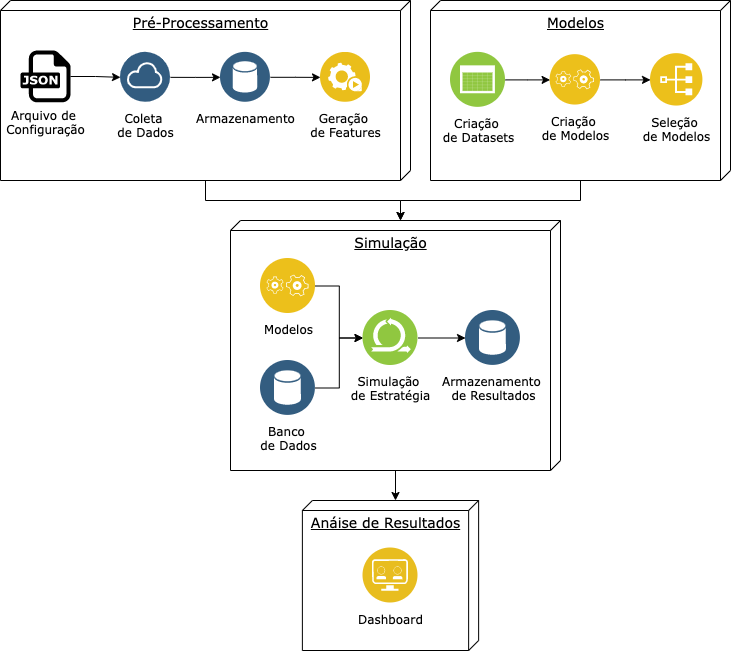
\includegraphics[scale=0.52]{resumo_projeto.png}
    \centering
    \caption{Estrutura do técnica do projeto}
    \label{fig:100}
\end{figure}

\paragraph{} Antes da execução do código principal, é necessário garantir que os modelos estão devidamente criados e acessíveis. Para isso, é importante a elaboração dos \textit{datasets} de cada ação a ser simulada, pois servem de entrada de dados para a criação e seleção dos modelos. A biblioteca \textit{multiprocessing} foi utilizada para minimizar o tempo total gasto nestas etapas.

\paragraph{} Após a criação dos modelos, tem-se início a etapa de pré-processamento de dados, onde ocorre a leitura e interpretação do arquivo de configuração para se obter o número de estratégias a executar, além dos ativos envolvidos e seus respectivos intervalos de tempo. Uma vez verificado no banco os dados já existentes, faz-se um \textit{download} apenas dos dados necessários. Se houver alguma atualização, as \textit{features} de uso geral são recalculadas e armazenadas no banco a fim de servir de insumo para as estratégias que estarão por vir.

\paragraph{} Completada a etapa de pré-processamento, inicia-se a simulação das estratégias. O arquivo de configuração foi projetado para ser capaz de designar diversas estratégias de parâmetros distintos a uma mesma ordem de execução de programa. Também fez-se uso da biblioteca \textit{multiprocessing} para paralelizar as simulações, cujos resultados e estatísticas são salvas no banco para posterior análise.

\paragraph{} Por fim, é possível visualizar os resultados de forma clara através de uma aplicação secundária responsável por criar um \textit{dashboard} interativo.

\paragraph{} Em relação às tecnologias utilizadas, a aplicação foi desenvolvida em \textit{Python} com o apoio das bibliotecas \textit{yfinance}, \textit{pandas}, \textit{numpy}, \textit{scikit-learn}, \textit{multiprocessing}, \textit{matplotlib} e \textit{dash}. Foi estruturado um banco de dados PostgreSQL para armazenamento dos \textit{candlesticks} obtidos, das \textit{features} geradas e das estratégias simuladas. Também foi incorporado o uso de \textit{Docker} especificamente para a execução de estratégias sem a necessidade de configuração de ambiente.



\FloatBarrier
\section{Pré-Processamento}

\FloatBarrier
\subsection{Arquivo de Configuração}
\label{sub:conf_file}

\paragraph{} O Arquivo de Configuração é um arquivo no formato JSON responsável por configurar detalhadamente cada parâmetro da sequência de estratégias que se deseja executar. Uma ordem de execução do programa pode conter diversas simulações de estratégias, que são configuradas neste Arquivo. A Figura \ref{fig:101} mostra sua estrutura.

\begin{figure}[!htb]
    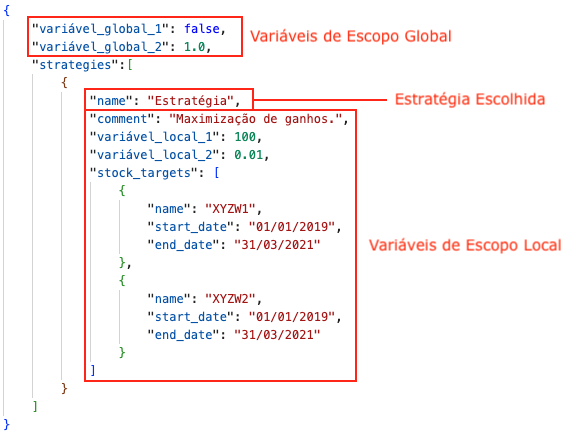
\includegraphics[scale=0.50]{config_file_estrutura.png}
    \centering
    \caption{Estrutura do Arquivo de Configuração}
    \label{fig:101}
\end{figure}

\paragraph{} Nota-se que no topo são listados os parâmetros de uso geral, ou variáveis de escopo global, de cujos valores precedem quaisquer outros listados a seguir, em caso de sobreposição. Em seguida abre-se o vetor de tipos de estratégias, onde o campo \textit{name} representa o nome da classe selecionada, sendo este o elemento que conecta o usuário ao tipo de estratégia desejada. Ressalta-se que este trabalho compreende apenas uma estratégia. Após a seleção do nome, são configurados os parâmetros internos da estratégia. A Tabela \ref{tab:3} da Seção \ref{sub:params_list} descreve todos os parâmetros disponíveis.

\paragraph{} Para se criar mais de um perfil de simulação, é necessário modificar o Arquivo conforme a Figura \ref{fig:102}. Automaticamente, o código interpreta que existe mais de uma simulação a executar, com todos os parâmetros em comum exceto aqueles em formato de listas. Caso haja mais de um parâmetro no formato de lista, seus comprimentos precisam ser iguais. No caso da Figura \ref{fig:102}, a primeira simulação utilizará os valores (100, 0.01) para o par (variável\_local\_1, variável\_local\_2), a segunda utilizará (200, 0.02) e assim sucessivamente.

\begin{figure}[!htb]
    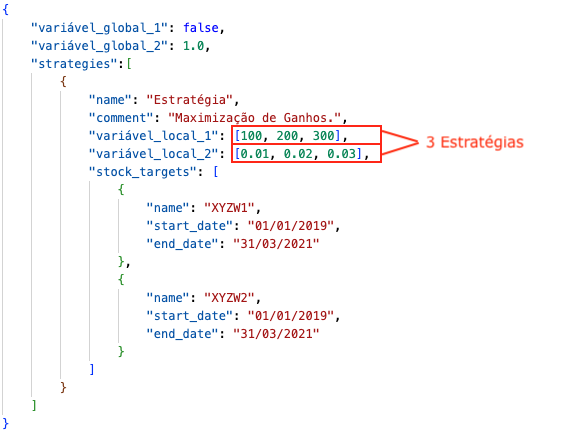
\includegraphics[scale=0.50]{config_file_mult_exec.png}
    \centering
    \caption{Arquivo de Configuração para Execuções Múltiplas}
    \label{fig:102}
\end{figure}



\FloatBarrier
\subsection{Coleta de Dados}
\label{coleta_de_dados}

\paragraph{} A Coleta de Dados ocorre através da biblioteca \textit{open-source} \textit{yfinance} \cite{yfinance}, uma ferramenta não oficial que transmite dados públicos da plataforma \textit{Yahoo! Finance} \cite{yahoo_finance}, um subsistema da rede \textit{Yahoo!}.

\paragraph{} A escolha desta biblioteca como fonte primária de dados se deve principalmente pela facilidade de uso associada à ausência de custos. Contudo, alguns testes e verificações com outras fontes de dados evidenciaram destantagens relevantes, porém não impeditivas para uso. São elas:

\begin{itemize}
    \item Os valores de proventos que a biblioteca disponibiliza não são consistentes com as declarações dos sites das próprias companhias, portanto não podem ser utilizados por este projeto. Testes internos confirmaram a presença de diversos proventos corretamente apresentados e ajustados pelos respectivos desdobramentos acumulados. O problema é que os mesmos estavam misturados com alguns \textit{outliers} inexistentes na realidade, o suficiente para questionar o uso em escala (i.e., para vários ativos sem verificação individual). \color{red} HERALDO: Devo mostrar evidências do teste que corrobora esta afirmação? \colorend

    \item Os volumes de negociação disponibilizados não necessariamente coincidem com a plataforma TradingView em valores absolutos, porém coincidem em valores relativos (i.e., variação de volume dia após dia para um mesmo ativo), o que é suficiente para este trabalho. \color{red} HERALDO: (1) Na verdade, encontrei algumas evidências de que os valores relativos conferem, mas nenhum evidência de que não conferem. (2) Será que posso citar a plataforma TradingView? Ou melhor, devo tomar algum cuidado? \colorend

    \item \textit{Candlesticks} de janelas temporais inferiores à diária (\textit{intraday}) são disponibilizados, porém as limitações envolvidas inviabilizam seu uso, como: o limite de 730 dias para a busca dos dados; a inconsistência com os dados diários quanto ao volume; e a alguns \textit{bugs} como a ausência de \textit{candlesticks} em todo dia de parcial do pregão da B3 (Quarta-feira de Cinzas).
\end{itemize}

% Aqui fala da criação de candles semanais
% \paragraph{} Os dados obtidos são \textit{candlesticks} diários (OHLCV). Com a mesma facilidade, é possível adquirir janelas de tempo semanais, no entanto para evitar potenciais problemas de consistência de dados, as mesmas são calculadas internamente a partir da janela diária via comandos SQL\footnote{\textit{Structured Query Language}: Linguagem usada para administrar bancos de dados relacionais.}.

\paragraph{} Apenas os dados não existentes no banco são baixados via \textit{yfinance}. Para isso, um \textit{trigger}\footnote{Procedimento armazenado em um banco de dados que é chamado automaticamente sempre que ocorre um evento.} é acoplado às tabelas de \textit{candlesticks} e acionado sempre que operações de \textit{insert}, \textit{update}, \textit{delete} e \textit{truncate} são realizadas. Quando ativado, ele chama uma função responsável por atualizar a tabela de \textit{status}, que registra o intervalo de tempo representado nas tabelas de \textit{candlesticks} para cada \textit{ticker} envolvido. Deve-se ressaltar que os devidos cuidados foram tomados para evitar buracos entre intervalos de tempo não adjacentes. Portanto, apenas uma consulta à tabela de \textit{status} é executada para se verificar a necessidade de \textit{download} de novos dados.



\FloatBarrier
\subsection{Armazenamento de Dados}

\paragraph{} O Armazenamento de Dados é realizado por um banco de dados \textit{PostgreSQL}, criado com o objetivo de salvar: os resultados das simulações; as \textit{features} de uso geral; e os \textit{candlesticks} obtidos. As vantagens de um banco de dados em relação a um arquivo CSV ou a uma planilha de Excel dispensam comentários. Contudo, quanto ao escopo deste trabalho, pode-se mencionar os seguintes pontos:

\begin{itemize}
    \item Fácil acesso aos resultados das simulações de forma estruturada e consistente, recurso este utilizado pela aplicação que gera o \textit{dashboard}.
    \item Economia de processamento devido ao armazenamento das \textit{features} de uso geral, uma vez que estratégias simuladas não necessitam recalculá-las a cada execução.
    \item Independência da plataforma \textit{Yahoo! Finance} para o caso de não continuidade dos dados ou qualquer alteração repentida.
    \item Diminuição do tráfego na rede pela persistência dos \textit{candlesticks} já obtidos.
\end{itemize}

% Aqui fala da criação de candles semanais
% \paragraph{} Os \textit{candlesticks} semanais são calculados via \textit{query} SQL para garantir a consistência dos dados, já que a possibilidade de inconsistência se fez presente entre dados \textit{intraday} e diários, conforme mencionado na Seção \ref{coleta_de_dados}.

\paragraph{} A figura \ref{fig:103} mostra o ERD\footnote{\textit{Entity-Relationship Diagram}. Em português: Diagrama de Entidade Relacionamento.} do banco. Os \textit{scripts} de criação e população inicial do banco de dados podem ser encontrado em \cite{github_projeto}. \color{red} HERALDO: (1) Vale a pena mostrar o ERD do banco? (2) Devo mencionar as constraints de banco que garantem consistência, como por exemplo a comparação do preço máximo de um candle com seus outros valores a fim de garantir que este de fato é máximo? Preços não negativos, valores não nulos, etc. \colorend

\begin{figure}[!htb]
    
\includegraphics[scale=0.90]{no_image.jpeg}
    \centering
    \caption{ERD do Banco de Dados}
    \label{fig:103}
\end{figure}



\FloatBarrier
\subsection{Geração de \textit{Features} de Uso Geral}
\label{sub:features}

\paragraph{} As \textit{Features} de Uso Geral são características derivadas dos \textit{candlesticks} que podem auxiliar qualquer decisão interna de uma estratégia, porém seu objetivo principal está no suporte à escolha do momento de entrada apropriado nas operações, o que é fundalmentalmente a responsabilidade do modelo de \textit{Machine Learning}. Como podem ser utilizadas por diversas estratégias, são calculadas antes do início das simulações e somente quando há necessidade, ou seja, quando os \textit{candlesticks} são inseridos pela primeira vez no banco ou quando são atualizados. Ao final dos cálculos, são armazenadas nas tabelas de \textit{features} para posteriores consultas durante as simulações.

\paragraph{} Ressalta-se que durante os cálculos, assim como em outras etapas, faz-se necessário atenção e cuidados quanto a erros de não-causalidade, que mesmo sendo sutis, podem influenciar drasticamente os resultados finais. \color{red} HERALDO: Devo omitir esse parágrafo? A intenção é dizer que não subestimei essa problema, portanto tomei cuidados a nível de implementação para evitá-lo. Por outro lado, talvez essa preocupação já esteja subentendida, sendo desnecessário enfatizá-la. \colorend

\paragraph{} As \textit{features} de Uso Geral utilizadas são:

\begin{itemize}
    \item \sout{Média Móvel Exponencial de 17 períodos no gráfico diário.} \\
    \color{red} HERALDO: Feature original do André Moraes. Não utilizada mais nos modelos. \colorend

    \item \sout{Média Móvel Exponencial de 72 períodos no gráfico diário.} \\
    \color{red} HERALDO: Feature original do André Moraes. Não utilizada mais nos modelos. \colorend

    \item \sout{Média Móvel Exponencial de 72 períodos no gráfico semanal.} \\
    \color{red} HERALDO: Feature original do André Moraes. Não utilizada mais nos modelos. \colorend

    \item \sout{\textit{Flag} de Tendência de Alta.} \\
    \color{red} HERALDO: Feature original do André Moraes. Não utilizada nos modelos DA FORMA QUE O ANDRÉ USA, por isso o risco no texto. Ele se baseia em picos e vales ascendentes para justificar uma tendência de alta (de acordo com a teoria de Dow). A nível de código, a estratégia mais simples é comparar os últimos 2 picos de mínimo e 2 picos de máximo, verificar se um é maior que o outro com alguma margem de tolerância, que se caracteriza tendência de alta. Porém essa informação é ruidosa, principalmente em mercados em consolidação (=muito lateralizados). O que ocorre na prática do André é que não são só os ultimos 4 picos que são analisados. Primeiro, ele já tira uma noção visual se o mercado anda em consolidação, isso requer olhar uma quantidade variável de picos que possuem algum grau de proximidade nas magnitudes, mas se comportam entre linhas de suporte e resistência. Quantos dias os picos passados devo olhar para medir a consolidação? (pergunta retórica). Se uma ação vem em tendência de baixa, por exemplo, ele não espera exatamente o par perfeito de 4 picos ascendentes para dizer se o mercado está em alta, muitas vezes porque o quarto pico ainda nem se formou consistentemente. Os testes que fiz foram baseados em uma identificação de picos, que ficou bem implementada, porém tem um atraso de 9 dias para identificar qualquer pico. Enfim, embora possível fazer um flag de tendencia de alta, não é trivial uma boa métrica fidedigna ao André, seguindo esta lógica. \colorend

    \item \sout{\textit{Stop Loss} no último pico de rompimento/reversão de tendência (Pressupõe preço de compra definido).} \\
    \color{red} HERALDO: Não utilizado mais pois era feature do André Moraes. Em particular, essa não é trivial de se calcular e foi uma das quais distanciou a simulação feita da estratégia real do André. Os picos relevantes que retratam a memória do mercado muitas vezes estão relacionados a acontecimentos notáveis, como crises financeiras, acidentes industriais, relatórios jurícos, escândalos, aquisições novas, etc. O André pode não avaliar os acontecimentos menores na escolha do stop por ser grafista e não estar inteiramente ligado nas notícias, mas leva em consideração os mais marcantes. Como análise de notícias está completamente fora do escopo, obter o grau de importância de um pico com alguma precisão requer no mínimo olhar os dados intraday (seção de coleta de dados explica porque não usei) e avaliar o volume de negociações na regiões. Contudo, idealmente deve-se olhar o livro de ofertas para tirar métricas das forças de compra e de venda, talvez aliadas ao volume de negociação e assim obter um valor razoável. Quando implementei na tentativa de simular o André, usei simplemente o pico mais próximo abaixo do preço de compra, dado uma distância mínima de 1\%. Em resumo, acho que foi mais uma métrica que contribui para uma estratégia ruim, por isso o abandono. \colorend

    \item \textbf{\textit{Flag} de Identificação de Crises} \\ \\
        \textit{Flag} criado para prever crises financeiras através da identificação de anomalias nos volumes de negociação e nas quedas dos preços. Seu objetivo é impedir que o modelo de ML entre em qualquer operação durante sua presença.

        Para o cálcula das anomalias de volume (Equação \ref{eq:20}), utiliza-se a média \begin{math} \overline{V} \end{math} e o desvio padrão \begin{math} \sigma_V \end{math} do volume de negociações dos últimos 60 dias úteis, junto com o volume \begin{math} V \end{math} do dia corrente. Adiciona-se um efeito de inércia de 2 dias úteis consecutivos para ativação do \textit{flag}.

        Já o cálculo das anomalias de queda de preços (Equação \ref{eq:150}), utiliza-se a média dos preços médios \begin{math} \overline{P_{mid}} \end{math} e seu desvio padrão \begin{math} \sigma_{P_{mid}} \end{math}, ambos relativos aos últimos 20 dias úteis e combinados com o preço médio \begin{math} P_{mid} \end{math} do dia corrente.

        \begin{equation} \label{eq:20}
            V_{anomaly(i)} = \begin{cases} 1, & \mbox{se } V_{(i)} > \overline{V} + \sigma_V \quad \textrm{e} \quad V_{(i-1)} > \overline{V} + \sigma_V \\
                0, & \mbox{caso contr\'ario} \end{cases}
        \end{equation}

        \begin{equation} \label{eq:22}
            P_{mid} = \dfrac{P_{open} + P_{close}}{2}
        \end{equation}

        \begin{equation} \label{eq:150}
            P_{anomaly(i)} = \begin{cases} 1, & \mbox{se } P_{mid(i)} < \overline{P_{mid}} + \sigma_{P_{mid}} \quad \\
                0, & \mbox{caso contr\'ario} \end{cases}
        \end{equation}

        O \textit{Flag} de Identificação de Crises (Equação \ref{eq:21}) é ativado quando ambas as anomalias de volume e de queda de preço estão ativadas. Caso essa condição não se mantenha mais a partir de um determinado instante, há uma inércia de 8 dias úteis para persistência do \textit{flag} de Crises.

        \begin{equation} \label{eq:21}
            F_{crisis(i)} = \begin{cases} 1, & \mbox{se } V_{anomaly(i)} = 1 \quad \textrm{e} \quad P_{anomaly(i)} = 1 \\
                1, & \mbox{se } (V_{anomaly(i)} = 0 \; \textrm{ou} \; P_{anomaly(i)} = 0) \; \textrm{e} \; F_{crisis(i-1)} = 1 \; (8 \textrm{m\'ax}) \\
                0, & \mbox{caso contr\'ario} \end{cases}
        \end{equation}

        A Figura \ref{fig:104} ilustra a eficácia do \textit{flag}. Observa-se que os três gráficos presentes na imagem se referem respectivamente ao cálculo das anomalias de queda de preços, ao cálculo das anomalias de volumes e por fim, ao cálculo do \textit{flag} de Identificação de Crises. Pode-se perceber que o mesmo foi corretamente ativado durante o início da crise do Coronavírus, pouco antes de 01/03/2020. Também houve ativação perto de 01/09/2020, embora sem um motivo claro aparente, os preços das ações durante o intervalo e logo após enfrentam uma pequena zona de consolidação, ou de desaceleração da tendência de alta que antes se apresentava. Nesta região, não se deseja entrar em operações até que uma nova tendência se forme.

        \begin{figure}[!htb]
            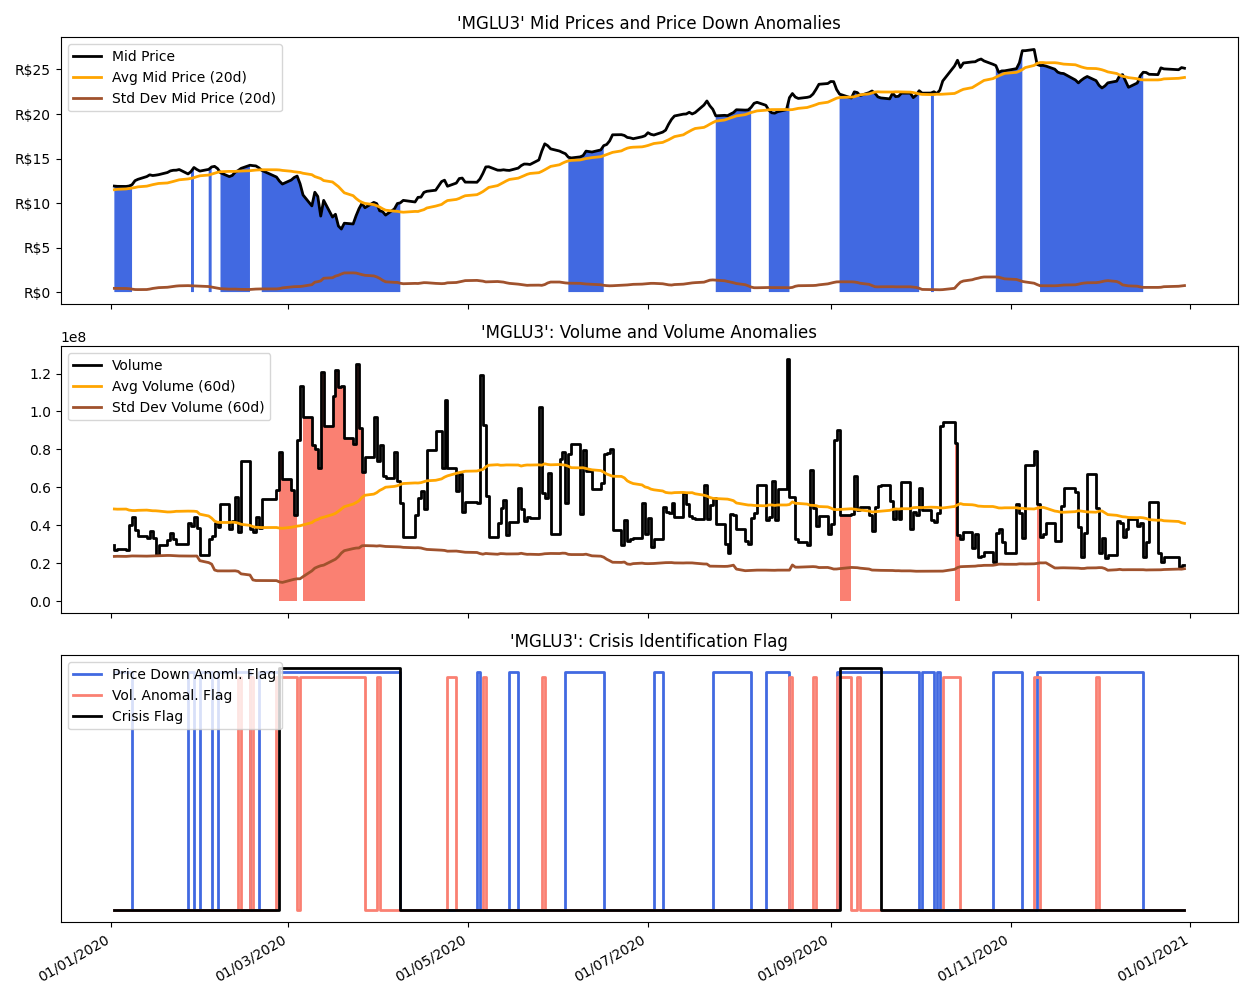
\includegraphics[scale=0.47]{crisis_flag_mglu3.png}
            \centering
            \caption{MGLU3 - \textit{Flag} de Identificação de Crises (01/01/2020 a 31/12/2020)}
            \label{fig:104}
        \end{figure}


    \item \textbf{\textit{Flag} de Tendência de Baixa} \\ \\
    Semelhante ao \textit{Flag} de Identificação de Crises, este \textit{Flag} também tem o objetivo de impedir entrada em operações pelo modelo de ML durante sua presença. No entanto, o critério é diferente. Primeiro, calcula-se a derivada dos preços médios \begin{math} \dot{P_{mid}} \end{math} entre o dia corrente e o anterior normalizado pela média dos preços médios (Equações \ref{eq:22} e \ref{eq:23}). Em seguida, ajusta-se um filtro digital IIR passa-baixas de coeficiente de amortecimento \begin{math} \alpha \end{math} (Equação \ref{eq:24}). Por fim, acrescenta-se um efeito de inércia de 3 dias úteis consecutivos para persistência do \textit{flag} em caso de ocorrência (Equação \ref{eq:25}). \color{red} HERALDO: Devo adicionar na fundamentação um tópico breve falando sobre filtro digital IIR passa-baixas e mostrando de onde vem essa fórmula? \colorend

    \begin{equation} \label{eq:23}
        \dot{P_{mid(i)}} = \dfrac{ P_{mid(i)} - P_{mid(i-1)} }{ \dfrac{1}{2}(P_{mid(i)} + P_{mid(i-1)}) }
    \end{equation}

    \begin{equation} \label{eq:24}
        \dot{P_{mid\_LPF(i)}} = \alpha \dot{P_{mid(i)}} + (1 - \alpha) \dot{P_{mid\_LPF(i-1)}},  \quad \textrm{onde} \quad 0 \le \alpha \le 1
    \end{equation}

    \begin{equation} \label{eq:25}
        F_{downtrend(i)} = \begin{cases} 1, & \mbox{se } \dot{P_{mid\_LPF(i)}} < 0 \\
            1, & \mbox{se } \dot{P_{mid\_LPF(i)}} \ge 0 \  e \  F_{downtrend(i-1)} = 1 \  \textrm{(3 m\'ax)} \\
            0, & \mbox{caso contr\'ario} \end{cases}
    \end{equation}

    Foi utilizado \begin{math} \alpha = 0.10 \end{math}, pois trantando-se de \textit{flag} que pode impedir diretamente o fluxo de negociações, prioriza-se um baixo ruído ao tempo de resposta.

    A Figura \ref{fig:109} ilustra a eficácia do \textit{Flag} de Identificação de Tendência de Baixa. Durante os maiores intervalos nos quais o \textit{Flag} esteve ativo, o preço se encontrou em queda. Por outro lado, quando verificado os intervalos menores, é mais comum a presença de falsos positivos.

    \begin{figure}[!htb]
        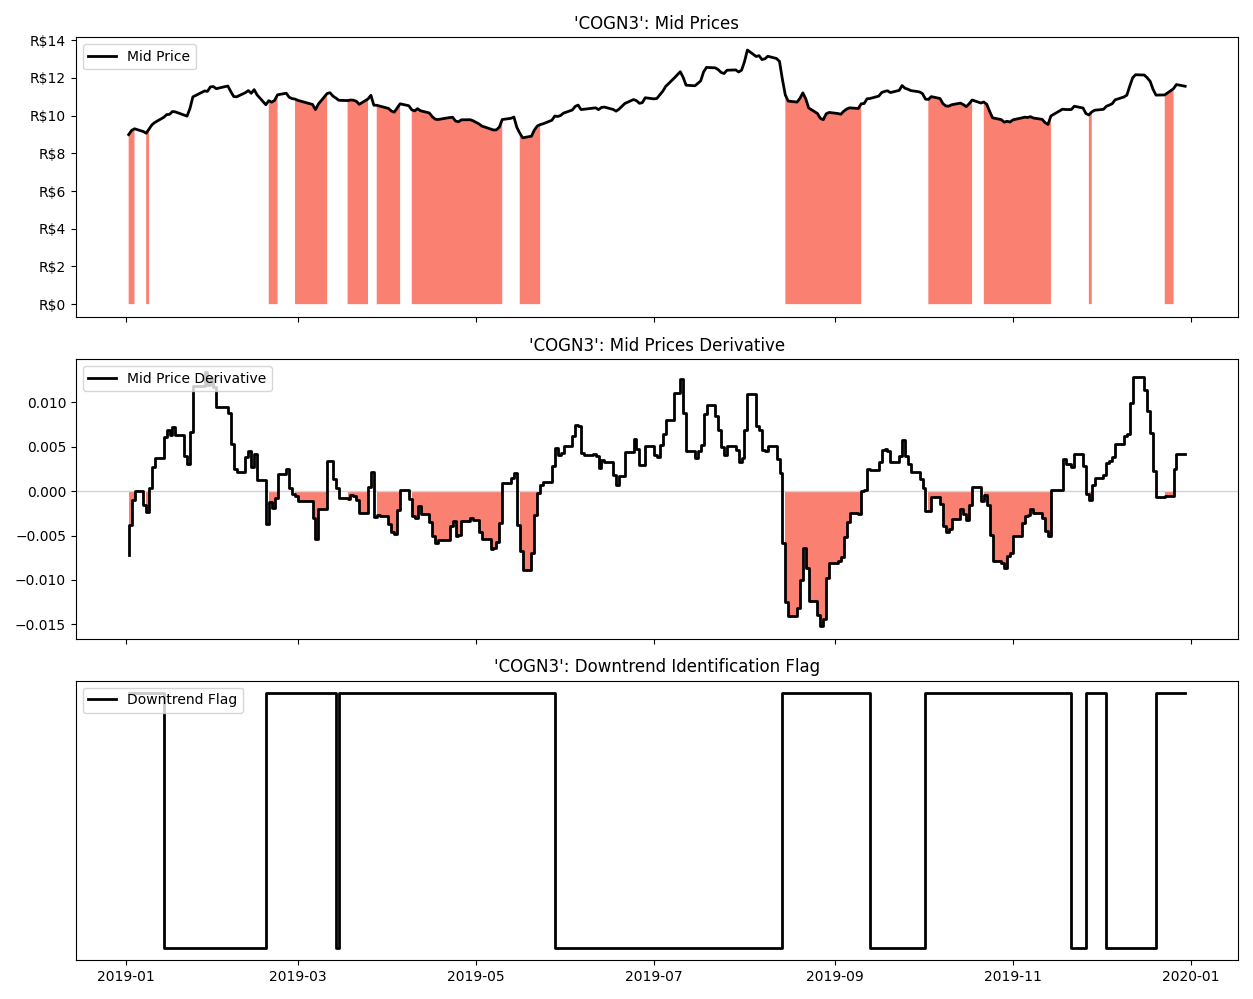
\includegraphics[scale=0.47]{downtrend_flag_cogn3.png}
        \centering
        \caption{COGN3 - \textit{Flag} de Identificação de Crises (01/01/2019 a 31/12/2019)}
        \label{fig:109}
    \end{figure}

    \item \textbf{Risco Mínimo} \\ \\
    O Risco Mínimo é uma \textit{feature} de suporte à escolha do risco de entrada em uma operação, não sendo assim consumido diretamente pelo modelo de ML. Ressalta-se que o conceito de risco no escopo deste trabalho está relacionado à diferença de valor no qual o \textit{stop loss} é colocado abaixo do preço de compra (Equação \ref{eq:51}). A escolha do risco também implica no valor do preço alvo de uma operação, pois o mesmo é definido como 3 vezes a magnitude do risco escolhido, percentualmente acima do preço de compra (ver Seção \ref{sub:estrutura}). A fórmula é composta por uma parcela fixa somada a uma parcela variável, conforme mostrado pela Equação \ref{eq:30}.

    \begin{equation} \label{eq:30}
        Risk_{min} = Risk_{min_f} + Risk_{min_v}
    \end{equation}

    Seja \begin{math} P_{\Delta} \end{math} a diferença entre o preço máximo e mínimo de um \textit{candle} (Equação \ref{eq:31}), pode-se definir \begin{math} Risk_{min_f} \end{math} como o valor mínimo de risco necessário para superar as oscilações diárias dos preços dos últimos 20 dias úteis (Equação \ref{eq:32}). Nota-se que \begin{math} \sigma_{P_{\Delta}} \end{math} é o desvio padrão relativo aos últimos 20 dias úteis.

    \begin{equation} \label{eq:31}
        P_{\Delta} = P_{high} - P_{low}
    \end{equation}

    \begin{equation} \label{eq:32}
        Risk_{min_f} = \dfrac{ \sigma_{P_{\Delta}} }{ P_{mid} }
    \end{equation}

    A parcela variável \begin{math} Risk_{min_v} \end{math} está associada à tendência de queda de preço no curto prazo. Seu cálculo é realizado a partir da derivada de preços ajustada por um filtro digital IIR passa-baixas (Equações \ref{eq:24} e \ref{eq:33}), onde \begin{math} \alpha \end{math} é o coeficiente de amortecimento. O sinal negativo indica que quanto maior a tendência de queda, maior precisa ser o risco associado.

    \begin{equation} \label{eq:33}
        Risk_{min_v} = - \dot{P_{mid\_LPF(i)}}
    \end{equation}

    Diferentemente do \textit{Flag} de Tendência de Baixa, foi utilizado \begin{math} \alpha = 0.30 \end{math}, uma vez que neste caso é mais interessante uma resposta rápida a um baixo ruído.

    Por fim, adicionou-se um segundo filtro de passa-baixas de \begin{math} \alpha = 0.10 \end{math} apenas aos movimentos de descida dos valores de \begin{math} Risk_{min} \end{math} com o objetivo de aumentar a cautela durante momentos mais turbulentos do mercado.

    As Figuras \ref{fig:400} e \ref{fig:105} e mostram os resultados do algoritmo para dois papéis de comportamentos distintos: MGLU3 representando um companhia com foco em alto crescimento, portanto mais volátil; e ABEV3 representando uma companhia já bem consolidada no mercado, portanto menos volátil. \color{red} HERALDO: Precisa de alguma citação aqui para suportar as afirmações feitas? \colorend \\

    \begin{figure}[!htb]
        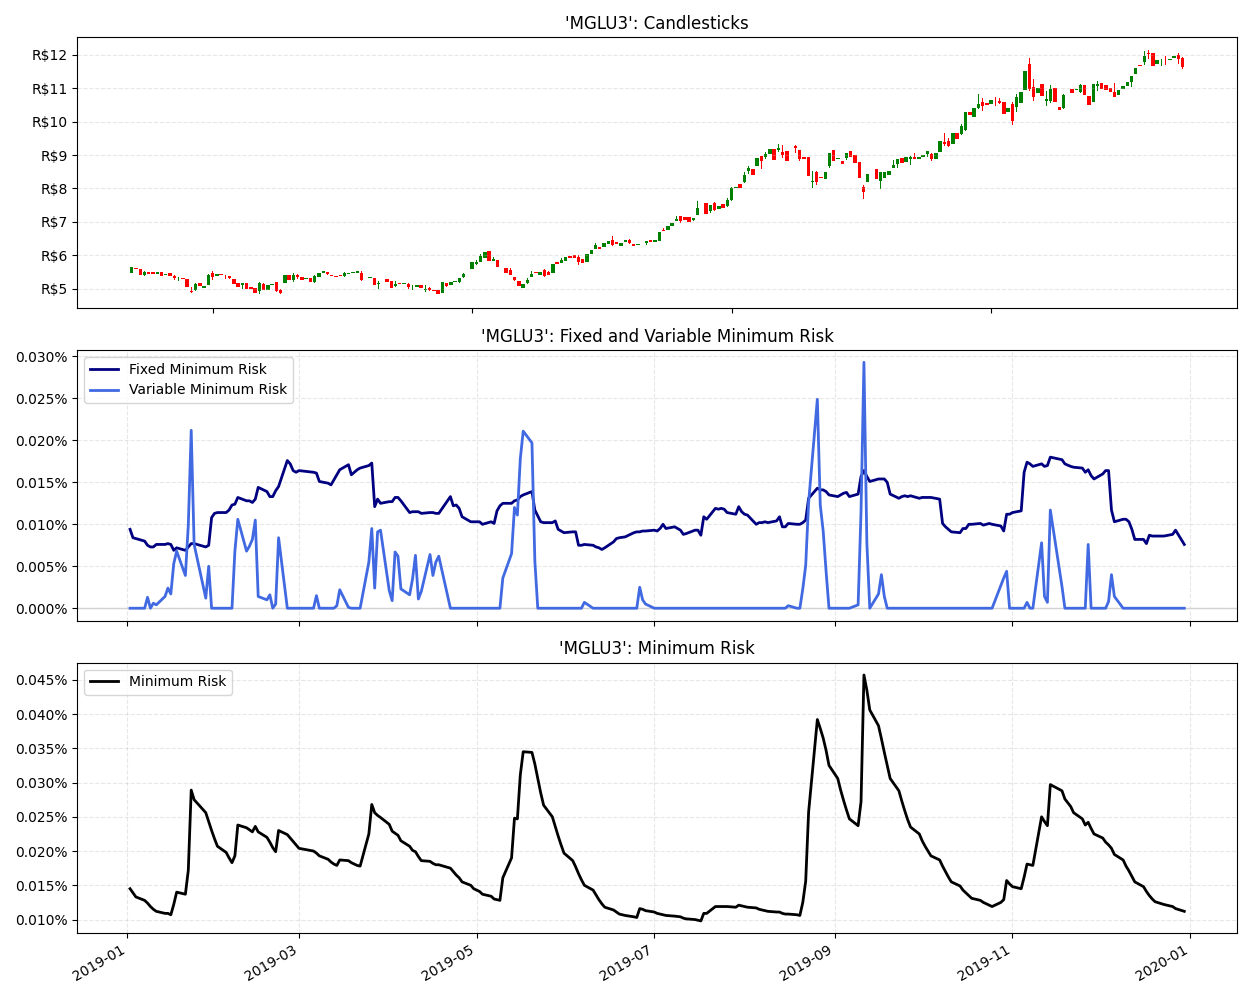
\includegraphics[scale=0.41]{min_risk_mglu3.png}
        \centering
        \caption{MGLU3 - Risco Mínimo (01/01/2019 a 31/12/2019)}
        \label{fig:400}
    \end{figure}

    \begin{figure}[!htb]
        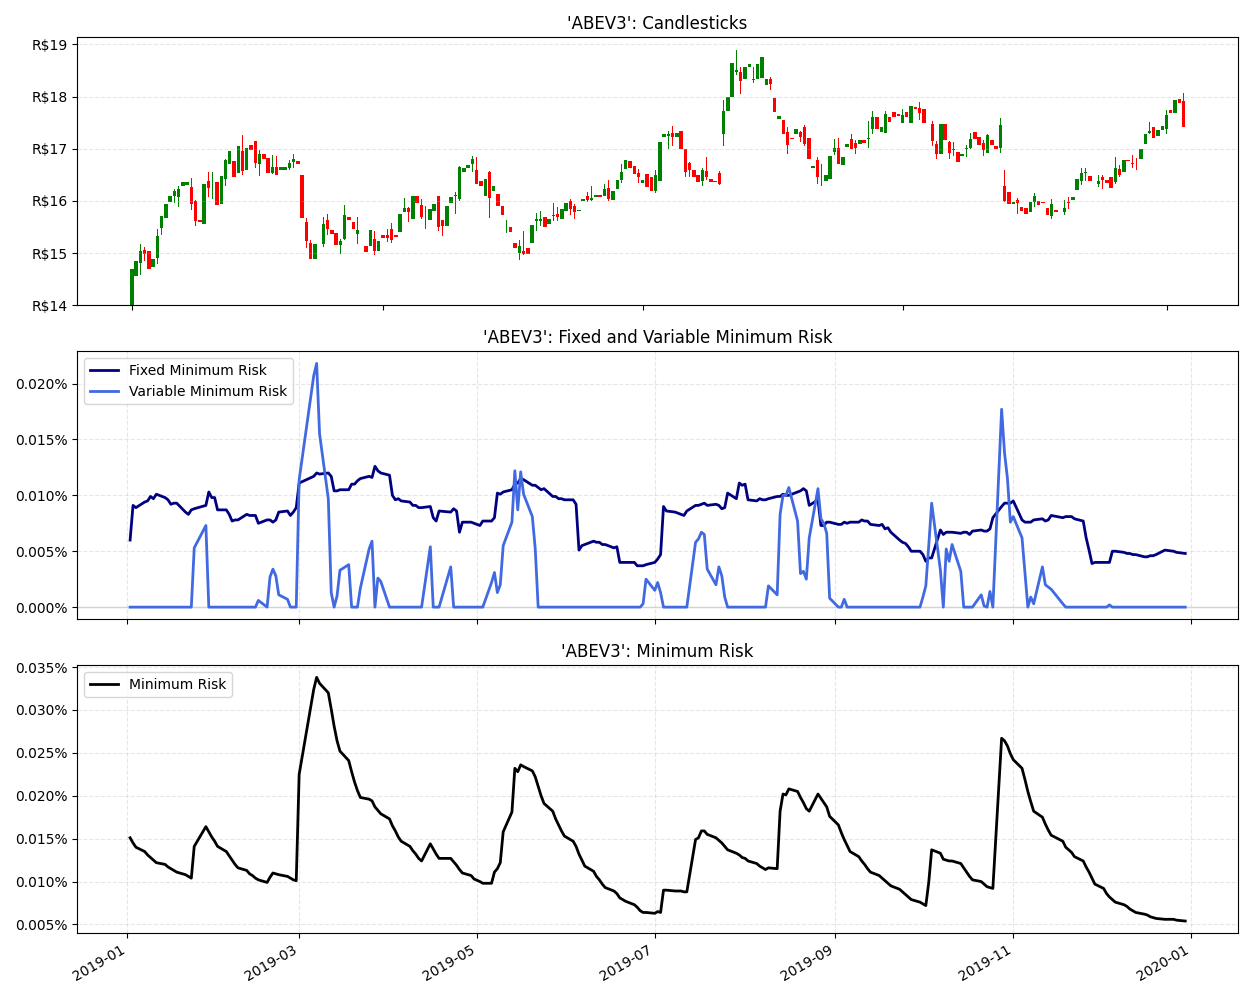
\includegraphics[scale=0.41]{min_risk_abev3.png}
        \centering
        \caption{ABEV3 - Risco Mínimo (01/01/2019 a 31/12/2019)}
        \label{fig:105}
    \end{figure}


    \item \textbf{Risco Máximo} \\ \\
    O Risco Máximo é uma \textit{feature} de suporte à escolha do risco de entrada em uma operação, não sendo assim consumido diretamente pelo modelo de ML. Ressalta-se que o conceito de risco no escopo deste trabalho está relacionado à diferença de valor no qual o \textit{stop loss} é colocado abaixo do preço de compra (Equação \ref{eq:51}). A escolha do risco também implica no valor do preço alvo de uma operação, pois o mesmo é definido como 3 vezes a magnitude do risco escolhido, percentualmente acima do preço de compra (ver Seção \ref{sub:estrutura}). A ideia central está na análise estatística das subidas de preços entre os últimos picos identificados dentro do intervalo de 80 dias úteis.

    Para se iniciar o cálculo, primeiro é necessário a criação de um um algoritmo de identificação de picos, conforme mostrado pela Figura \ref{fig:106}. O método usa uma janela móvel de \begin{math} W = 5 \end{math} \textit{candles} que corre dia após dia até a data corrente e atribui 1 voto de máximo e 1 voto de mínimo aos preços de máximo e preços de mínimo encontrado na janela, respectivamente. Em todos os passos, o primeiro e o último \textit{candle} da janela nunca recebem votos devido à falta de um \textit{candle} adjacente. São elegíveis à picos apenas os \textit{candles} que obtiveram um mínimo de \begin{math}  floor(W / 2) = 2 \end{math} votos. Ao final, garante-se a alternância entre máximos e mínimos locais através da remoção de picos consecutivos de um mesmo tipo.

    \begin{figure}[!htb]
        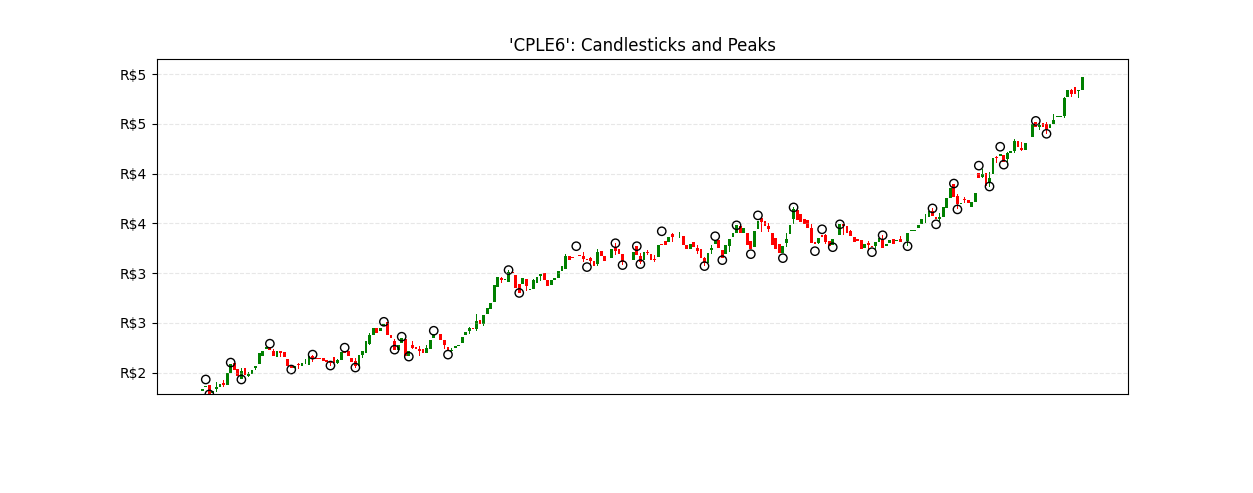
\includegraphics[scale=0.47]{peaks_cple6_w_5.png}
        \centering
        \caption{CPLE6 - Algoritmo de identificação de picos (01/01/2019 a 31/12/2019)}
        \label{fig:106}
    \end{figure}

    % O algoritmo implementado cumpre seu propósito pois se assemelha ao método grafista de identificação de picos \cite{moraes2007se}. O valor da janela de 17 \textit{candles} foi escolhido devido a teoria do Phi Cube \cite{moraes2007se}. \color{red} HERALDO: Para uma identificação de picos Embora tenha me baseado na teoria do Phi Cube por causa do André, confesso que não me sinto confortável em citá-la, pois ela me parece uma tentativa desesperada de trazer algum critério a um processo muito mais caótico e complexo. \colorend

    % Depois da identificação de picos, extraem-se as \begin{math} n \end{math} subidas de preços de cada mínimo para o máximo consecutivo no período designado, normalizados pelo pico de mínimo (Figura \ref{fig:107} e Equação \ref{eq:40}). Em seguida, calcula-se a média \begin{math} \overline{C_{LPF(i)}} \end{math} e o desvio padrão \begin{math} \sigma_{C_{LPF(i)}} \end{math} com um filtro digital IIR passa-baixas (Equações \ref{eq:41}, \ref{eq:42} e \ref{eq:43}). Finalmente, o Risco Máximo \begin{math} Risk_{max} \end{math} pode ser encontrado segundo a Equação \ref{eq:44}, onde \begin{math} G \end{math} é a constante de razão entre ganho e perda, cujo valor é constante e igual a 3 em todo o escopo deste trabalho.

    Depois da identificação de picos, extraem-se as \begin{math} n \end{math} subidas de preços de cada mínimo para o máximo consecutivo no período designado, normalizados pelo pico de mínimo (Figura \ref{fig:107} e Equação \ref{eq:40}). Por fim, o Risco máximo é obtido pelo cálculo da média \begin{math} \overline{C_{(i)}} \end{math} com um filtro digital IIR passa-baixas (Equações \ref{eq:41} e \ref{eq:42}).

    \begin{figure}[!htb]
        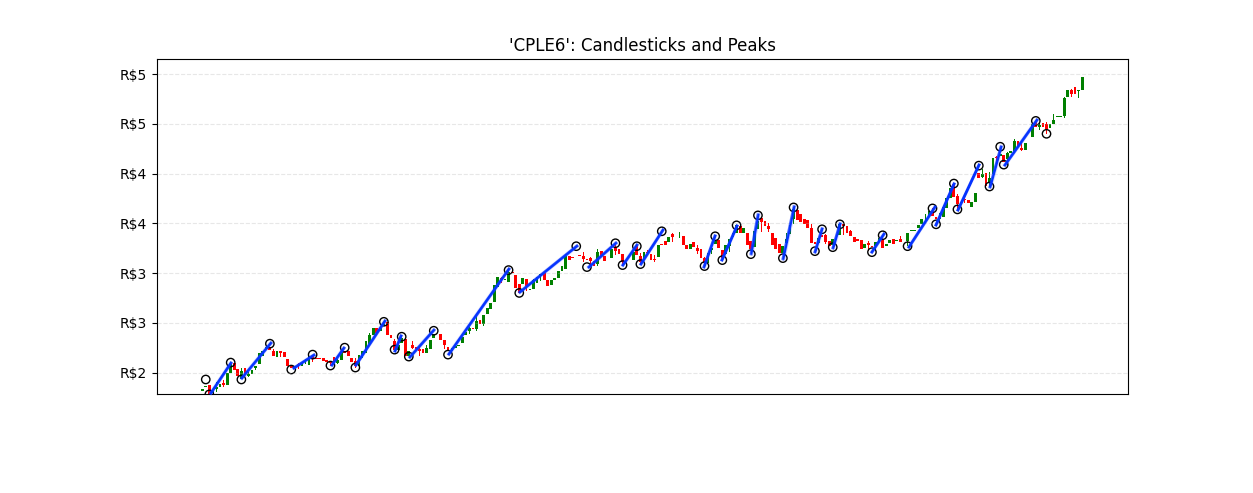
\includegraphics[scale=0.47]{peaks_with_marks_cple6_w_5.png}
        \centering
        \caption{CPLE6 - Subidas de preços entre picos (01/01/2019 a 31/12/2019)}
        \label{fig:107}
    \end{figure}

    \begin{equation} \label{eq:40}
        c_k = (P_{max(k)} - P_{min(k)}) / P_{min(k)}, \quad \textrm{onde } 0 < k \le n
    \end{equation}

    \begin{equation} \label{eq:41}
        \overline{C_{(i)}} = \dfrac{1}{n} \sum_{k=1}^{n} c_k
    \end{equation}

    \begin{equation} \label{eq:42}
        Risk_{max(i)} = \alpha \overline{C_{(i)}} + (1 - \alpha) Risk_{max(i-1)}
    \end{equation}

    % \begin{equation} \label{eq:43}
    %     \sigma_{C_{LPF(i)}} = \alpha \sigma_{C(i)} + (1 - \alpha) \sigma_{C_{LPF(i-1)}}
    % \end{equation}

    % \begin{equation} \label{eq:44}
    %     Risk_{max(i)} = \dfrac{1}{G} (\overline{C_{LPF(i)}} - 0.5\sigma_{C_{LPF(i)}}), \quad \textrm{onde } G = 3
    % \end{equation}

    % \begin{equation} \label{eq:44}
    %     Risk_{max(i)} = \dfrac{1}{G} (\overline{C_{LPF(i)}} - 0.5\sigma_{C_{LPF(i)}}), \quad \textrm{onde } G = 3
    % \end{equation}

    Foi utilizado \begin{math} \alpha = 0.50 \end{math}.

    As Figuras \ref{fig:108} e \ref{fig:270} mostram o Risco Máximo para os ativos MGLU3 e ABEV3, respectivamente.

    \begin{figure}[!htb]
        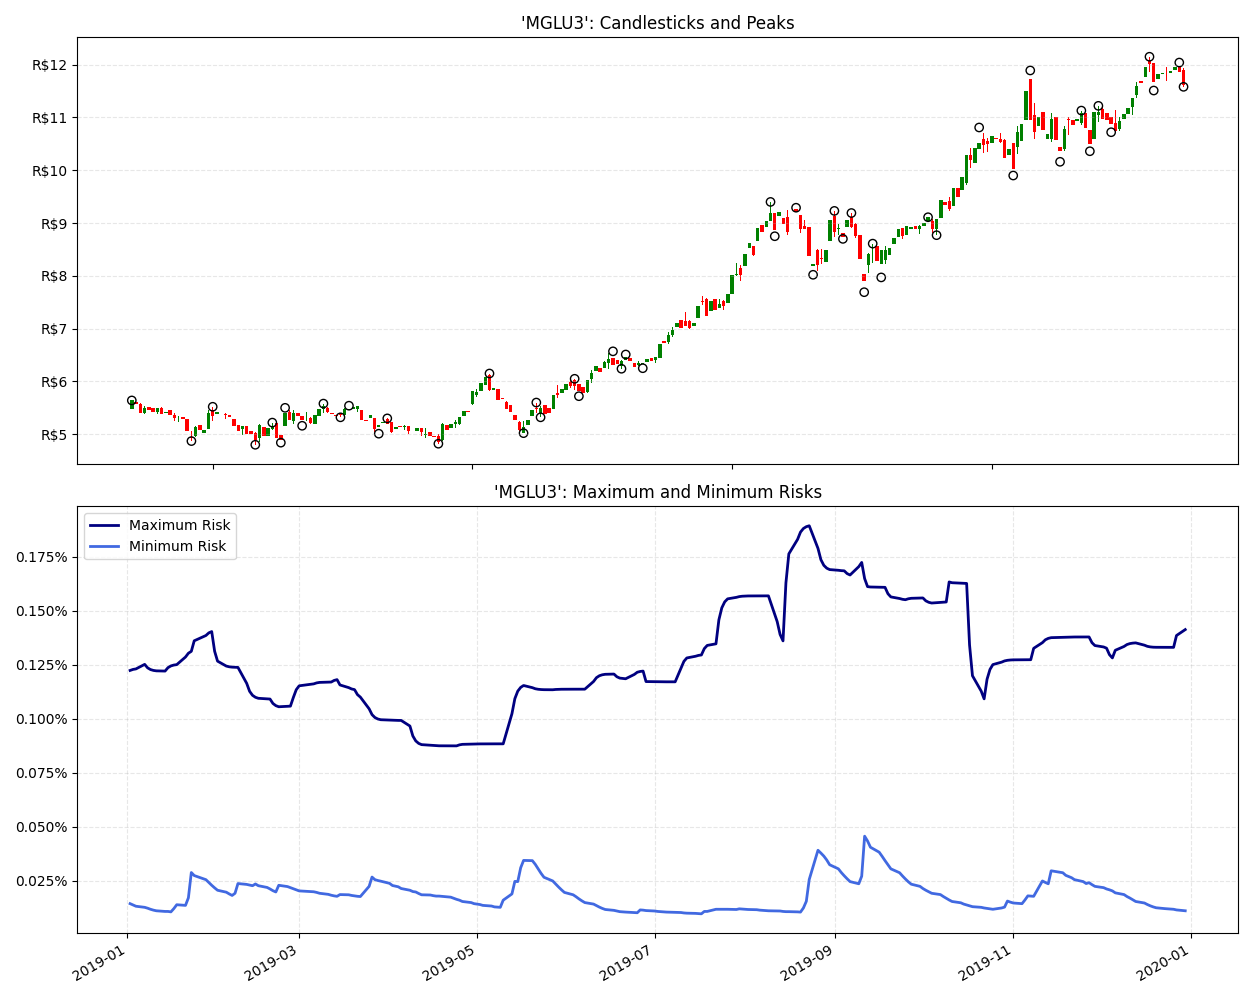
\includegraphics[scale=0.41]{max_risk_mglu3.png}
        \centering
        \caption{MGLU3 - Riscos Máximo e Mínimo (01/01/2019 a 31/12/2019)}
        \label{fig:108}
    \end{figure}

    \begin{figure}[!htb]
        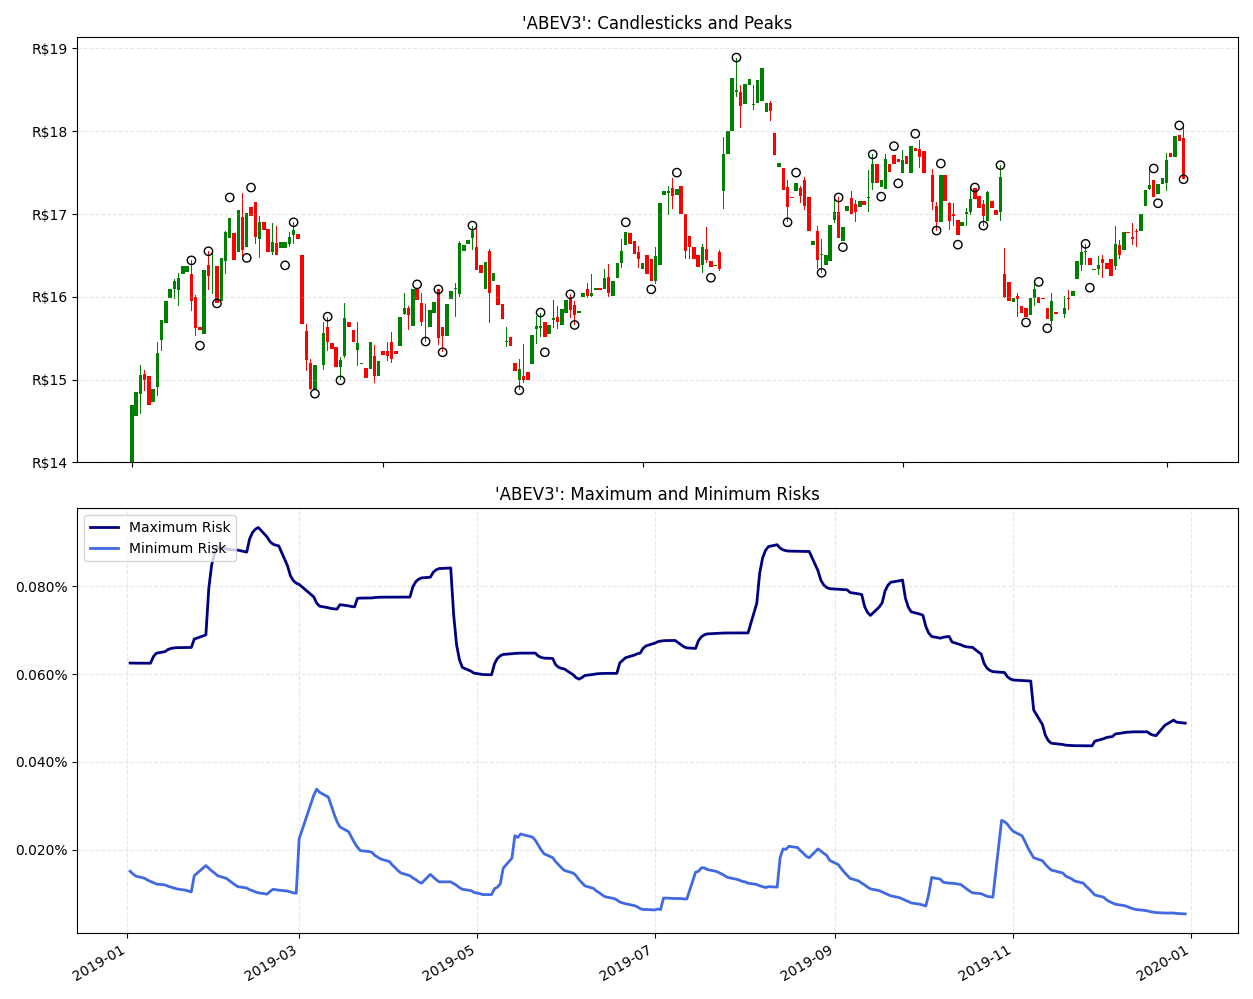
\includegraphics[scale=0.41]{max_risk_abev3.png}
        \centering
        \caption{ABEV3 - Riscos Máximo e Mínimo (01/01/2019 a 31/12/2019)}
        \label{fig:270}
    \end{figure}

\end{itemize}



\FloatBarrier
\section{Simulação de Estratégia}

\FloatBarrier
\subsection{Estrutura}
\label{sub:estrutura}

\paragraph{} O tema escolhido pelo presente trabalho permite uma enorme quantidade possíveis implementações, onde muitas se mostram como promissoras e interessantes de se explorar. No entanto, dar vida a um projeto de engenharia envolve a delimitação de um escopo, que necessariamente restringe as possibilidades. Dessa forma, a Estrutura na qual as estratégias são simuladas se baseia nas seguintes declarações:


\begin{itemize}
    \item Toda estratégia possui um \textbf{capital inicial}, que representa uma quantidade de capital pré-alocado para compra dos ativos financeiros. Essa quantia deve ser sempre respeitada ao longo da simulação de forma a não representar nunca um valor negativo.

    \item Toda estratégia deve possuir uma \textbf{carteira de ativos} (ou lista de ativos) com as respectivas datas iniciais e finais de validade, isto é, intervalos de tempo onde as operações podem ser realizadas. Embora sejam permitidos intervalos diferentes, é convencionado a mesma data de início e de fim para todos os papéis.

    \item Define-se uma  \textbf{operação} como o processo de compra única de um volume de ações de um ativo seguido pela venda de todo o volume comprado, independentemente do tempo, mesmo que esta ocorra em estágios. Nota-se que apenas a venda é cabível de ocorrer em estágios (i.e., venda parcial).

    \item Toda operação possui um \textbf{preço alvo} e um \textbf{\textit{stop loss}}. O preço alvo é um valor acima do preço de compra e o \textit{stop loss} é um valor abaixo do preço de compra. Quando o mercado atinge qualquer um dos dois valores, uma venda é disparada, encerrando a operação em vigor. No entanto, considera-se uma operação de sucesso aquela que encerrou por atingir o preço alvo e uma operação de falha aquela que encerrou por atingir o \textit{stop loss}.

    \item Uma estratégia pode possuir no máximo  \textbf{uma operação em vigência} para cada \textit{ticker} em sua bolsa de ativos, portanto para que uma segunda compra ocorra no momento em que já existem papéis adquiridos, é necessários vendê-los primeiro.

    \item A \textbf{razão entre ganho e perda} predetermina a relação entre o preço alvo e o \textit{stop loss} em qualquer operação. Ela indica a razão entre a diferença do preço alvo \begin{math} P_{target} \end{math} para o preço de compra \begin{math} P_{buy} \end{math} sobre a a diferença do preço de compra para o \textit{stop loss} \begin{math} P_{stop} \end{math} (Equação \ref{eq:50}). Seu valor é constante e igual a 3 em todo o escopo deste trabalho. \color{red} HERALDO: O valor de 3 veio do André. Devo citar ele aqui? Não achei uma referência direta disso em seu livro, porém tem nos vídeos. \colorend

    \begin{equation} \label{eq:50}
        G = \dfrac{P_{target} - P_{buy}}{P_{buy} - P_{stop}} = 3
    \end{equation}

    Utiliza-se o termo ``risco de uma operação" ou simplesmente ``risco" como sendo a diferença de valor no qual o \textit{stop loss} é colocado abaixo do preço de compra (Equação \ref{eq:51}). Por exemplo, se o preço de compra de uma operação é de R\$10,00 e o seu risco é de 5\%, então o \textit{stop loss} se encontra em R\$9,50 e o preço alvo em R\$11,50 necessariamente.

    \begin{equation} \label{eq:51}
        Risk = \dfrac{P_{buy} - P_{stop}}{P_{buy}}
    \end{equation}

    \item Não há \textbf{operações a descoberto}.
    \item Não há \textbf{operações alavancadas}.

\end{itemize}



\FloatBarrier
\subsection{Premissas}

\paragraph{} As Premissas são um conjunto de afirmações que visam complementar a Estrutura das simulações ao mesmo tempo que garantir a integridade dos resultados, muitas vezes optando pelo pior cenário em situações inconclusivas. São elas:

\begin{itemize}
    \item O momento de decisão de \textbf{entrada em uma operação} por uma estratégia ocorre durante a abertura de mercado do dia corrente, mais precisamente no instante em que o preço de abertura é definido.

    \item No dia que houver a compra de um ativo, não pode haver a venda do mesmo. Em outras palavras, o \textbf{período mínimo de duração de uma operação é de 1 dia útil}.

    \item A \textbf{venda por \textit{timeout}} ocorre quando o número máximo de dias de uma operações extrapola um valor definido (ver Seção \ref{sub:max_op_days})

    \item Devido a ausência de informações mais detalhadas que a janela de tempo diária, a seguinte ordem é priorizada durante a \textbf{venda de um ativo}:

    \begin{enumerate}
        \item Venda por \textit{stop loss}
        \item Venda parcial (caso habilitada)
        \item Venda por preço alvo
        \item Venda por \textit{timeout}
    \end{enumerate}

    \item Caso algum \textbf{preço de venda seja pulado}, ou seja, a descontinuidade entre o preço de abertura do dia corrente e o preço de fechamento do dia anterior não englobe o valor de venda, utiliza-se o preço de abertura do dia corrente. A única exceção acontece para a venda por \textit{timeout}, já que se trata de uma venda compulsória que sempre ocorre no preço de fechamento do dia designado.

\end{itemize}



\FloatBarrier
\subsection{Gerenciamento de Risco}
\label{sub:risk_man}

\paragraph{} Segundo André Moraes \cite{moraes2007se}, um bom Gerenciamento de Risco é essencial para a performance de uma estratégia. Afinal, não adianta obter uma alta taxa de acerto em operações de cujo lucro médio não compense as perdas acumuladas pelas operações que falham. Além disso, estar com o capital muito alocado em ativos de um único segmento é perigoso devido à exposição à fatores como falta de insumos industriais, mudanças na legislação, crises internas, instabilidade política, dentre outros.

\paragraph{} Para mitigar as questões levantadas, algumas medidas foram tomas inspiradas no trabalho de André Moraes \cite{moraes2007se}. São elas:

\begin{itemize}
    \item Diversificação de ativos em segmentos de mercado variados através da escolha de um alto número de \textit{tickers} na carteira, mais especificamente 71.
    \item Criação do Coeficiente de Risco-Capital\footnote{ou \textit{Risk-Capital Coefficient} (RCC)}
\end{itemize}

\paragraph{} O Coeficiente de Risco-Capital, definido pela Equação \ref{eq:60}, é uma constante que equilibra a relação entre o capital de entrada em uma operação e o risco escolhido. Seu valor é configurado previamente no Arquivo de Configuração (ver Tabela \ref{tab:3}) e vale para todos os ativos da carteira.

\begin{equation} \label{eq:60}
    RCC = Capital \times Risk
\end{equation}

\paragraph{} Durante uma simulação, a estratégia primeiro encontra o valor do risco desejado para entrar na operação, depois escolhe o capital a ser alocado. Dessa forma, a Equação \ref{eq:61} mostra de fato a aplicação do RCC. É evidente que quanto maior o risco envolvido, menor o capital a ser alocado e vice-versa.

\begin{equation} \label{eq:61}
    Capital = \dfrac{RCC}{Risk}
\end{equation}

\paragraph{} O RCC influencia diretamente no uso médio de capital de uma estratégia. Por um lado, um uso de capital baixo significa um mau aproveitamento do capital, o que leva a uma performance ruim. Por outro lado, muito uso de capital implica em pouco capital disponível para entrada em novas operações, o que também leva a uma performance ruim e instável, visto que a operação que iniciar imediatamente antes das demais leva quase todos o capital consigo.

\paragraph{} A Figura \ref{fig:550} mostra o gráfico da relação entre os indicadores de performance em função do RCC para os 71 \textit{tickers} da Tabela \ref{tab:5}. Nenhuma otimização foi adicionada. Nota-se no início do gráfico uma região de máximos locais em cada indicador, seguido por uma pequena queda até retomar novamente a subida dos valores. Percebe-se também que a partir do RCC de 1,88\%, o uso de capital está quase saturando. \color{red} HERALDO: Não sei explicar o motivo do mínimo local nos indicaroes. \color{black}

% Nota-se que abaixo do valor de RCC de aproximadamente 2,5\%, tanto o rendimento final quando índice de Sharpe e de Sortino estão crescentes, apesar das oscilações. Após esse valor, ambos possuem ainda uma subida, porém ao custo de bastante instabilidade.

\begin{figure}[!htb]
    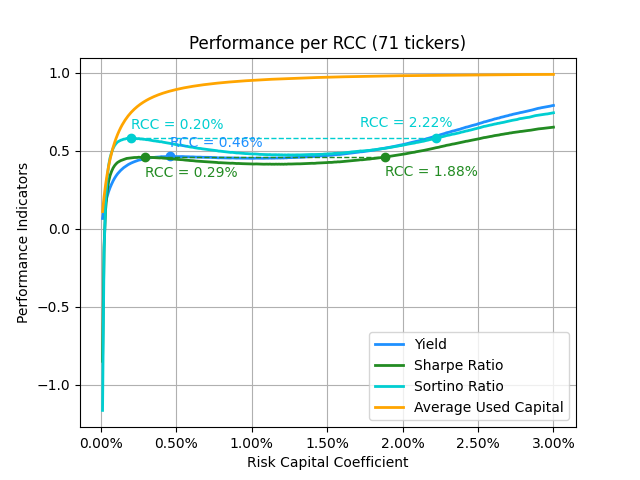
\includegraphics[scale=0.80]{performance_per_rcc_2.png}
    \centering
    \caption{Indicadores de performance em função do RCC (71 tickers: 01/01/2019 a 31/12/2021)}
    \label{fig:550}
\end{figure}

\paragraph{} Dentre as execuções que compõem a Figura \ref{fig:550}, extraiu-se os gráficos de uso de capital para as simulações de RCC=0.29\% e RCC=1,88\% (Figuras \ref{fig:551} e \ref{fig:552}, respectivamente). Nota-se o efeito de saturação causado pelo aumento significativo do RCC, que reduziu o número de operações totais de 3972 para 3390 pela falta de capital disponível em alguns intervalos. Por outro lado, operações longe da saturação receberam mais capital e como estas são mais expressivas, a performance geral foi maior.
% Antes era: "... reduziu o número de operações totais de 379 para 302 pela ..."

% \begin{figure}[!htb] % ID 315
%     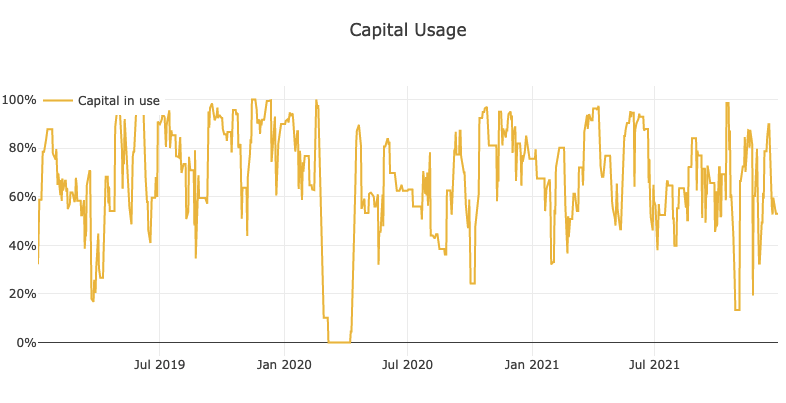
\includegraphics[scale=0.50]{rcc_capital_usage_08.png}
%     \centering
%     \caption{Uso de Capital (20 tickers, 01/01/2019 a 31/12/2021, RCC = 0,8\%)}
%     \label{fig:551}
% \end{figure}

% \begin{figure}[!htb] % ID 345
%     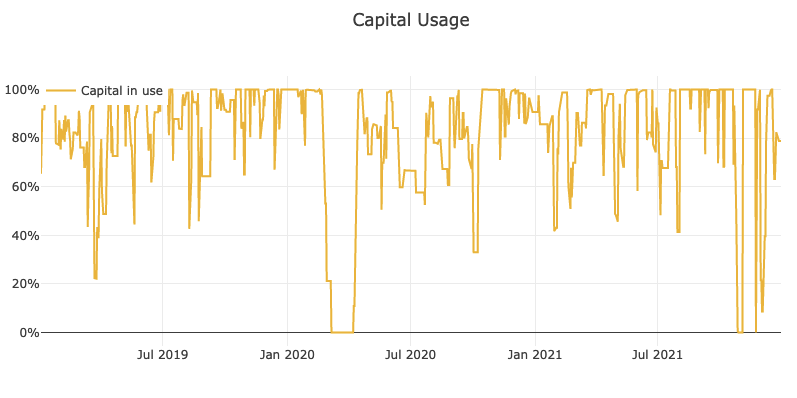
\includegraphics[scale=0.50]{rcc_capital_usage_20.png}
%     \centering
%     \caption{Uso de Capital (20 tickers, 01/01/2019 a 31/12/2021, RCC = 2,0\%)}
%     \label{fig:552}
% \end{figure}

\begin{figure}[!htb] % ID
    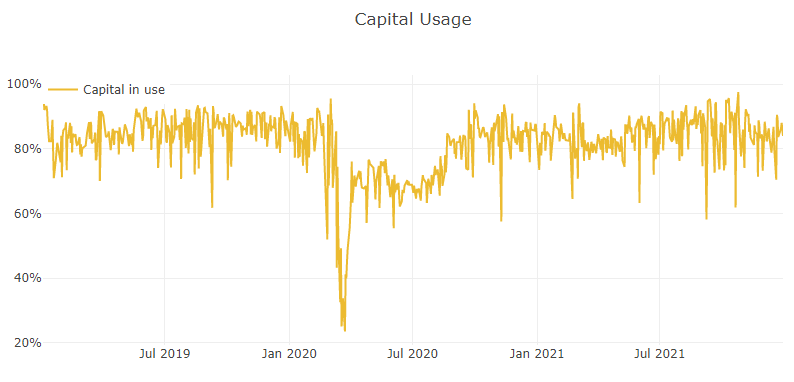
\includegraphics[scale=0.650]{rcc_capital_usage_00029.png}
    \centering
    \caption{Uso de Capital (71 tickers, 01/01/2019 a 31/12/2021, RCC = 0,29\%)}
    \label{fig:551}
\end{figure}

\begin{figure}[!htb] % ID
    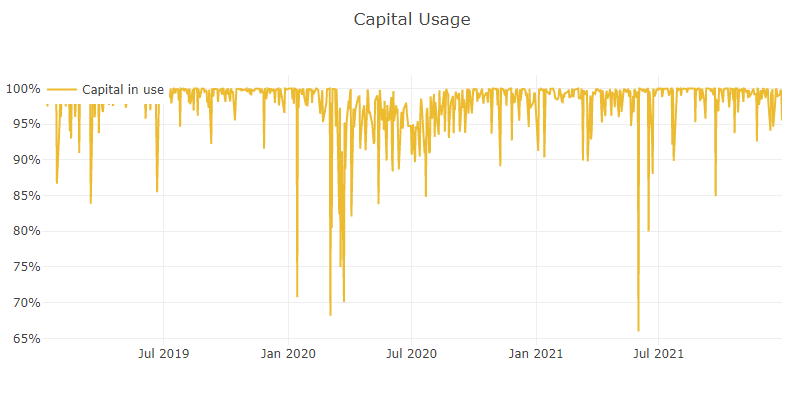
\includegraphics[scale=0.650]{rcc_capital_usage_00188.png}
    \centering
    \caption{Uso de Capital (71 tickers, 01/01/2019 a 31/12/2021, RCC = 1,88\%)}
    \label{fig:552}
\end{figure}

\paragraph{} Um problema geral e inerente à abordagem do RCC é a necessidade do conhecimento \textit{a priori} de um valor razoável. Ou seja, sem algumas simulações prévias, não há como se saber um valor ótimo ou pelo menos próximo dele. Uma forma de se atenuar esse problema é através da criação de um controle proporcional que aumente o RCC geral em função do baixo aproveitamento de uso de capital dos dias corridos e vice-versa. Essa alternativa também é chamada de RCC Dinâmico e abordada em mais detalhes na Seção \ref{sub:dynamic_rcc}.

% \paragraph{} A alta sensibilidade \textit{a priori} da performance em relação ao RCC é um condição indesejável. Da mesma forma, uma melhor distribuição do uso de capital ao longo do período de simulação inspirou a criação de um RCC Dinâmico, que é tratado em detalhes na Seção \ref{sub:dynamic_rcc} por se tratar de uma otimização.

\paragraph{} A Tabela \ref{tab:5} lista todos os 71 ativos escolhidos para simulação no escopo deste trabalho. Os critérios de escolha envolvem as seguintes preferências: diversidade de segmentos; disponibilidade da série temporal de dados a partir de 2013; e presença na composição do iBovespa em qualquer data. \color{red} HERALDO: Coloquei a tabela aqui pois foi o primeiro momento no qual foi relevante mencionar as 71 ações escolhidas, portanto aproveitei o gancho. Mas se houver outro lugar mais adequado, posso trocar. \colorend

\begin{table}[h!]
    \begin{center}
        \begin{tabular}{ cccccccc }
            \multicolumn{8}{c}{Ações Escolhidas (71)} \\
            \hline
            ABEV3 & ALPA4 & AMER3 & B3SA3 & BBAS3 & BBDC3 & BBDC4 & BBSE3 \\
            BEEF3 & BPAN4 & BRAP4 & BRFS3 & BRKM5 & BRML3 & CCRO3 & CIEL3 \\
            CMIG4 & COGN3 & CPFE3 & CPLE6 & CSAN3 & CSNA3 & CVCB3 & CYRE3 \\
            DXCO3 & ECOR3 & EGIE3 & ELET3 & ELET6 & EMBR3 & ENBR3 & ENEV3 \\
            ENGI11 & EQTL3 & EZTC3 & FLRY3 & GGBR4 & GOAU4 & GOLL4 & HYPE3 \\
            ITSA4 & ITUB4 & JBSS3 & JHSF3 & LAME4 & LCAM3 & LREN3 & MGLU3 \\
            MRFG3 & MRVE3 & MULT3 & PETR3 & PETR4 & POSI3 & PRIO3 & QUAL3 \\
            RADL3 & RENT3 & SANB11 & SBSP3 & SULA11 & TAEE11 & TIMS3 & TOTS3 \\
            UGPA3 & USIM5 & VALE3 & VIIA3 & VIVT3 & WEGE3 & YDUQ3
        \end{tabular}
        \caption{Ações Escolhidas}
        \label{tab:5}
    \end{center}
\end{table}



\FloatBarrier
\subsection{Risco de Entrada por Operação}
\label{sub:operation_risk}

\paragraph{} O Risco de Entrada por Operação é encontrado a partir de um valor intermediário entre o Risco Mínimo e o Risco Máximo.

\paragraph{} Pelo fato da metodologia de cálculo do Risco Máximo e do Risco Mínimo seguirem raciocínios diferentes (Seção \ref{sub:features}), podem ocorrer momentos nos quais a equação \begin{math} Risk_{max} < Risk_{min} \end{math} seja verdadeira, em outras palavras, as ondas de subida de preço entre picos no gráfico diário não compensem as oscilações inerentes ao ruído diário dos \textit{candlesticks}. Enquanto este evento ocorrer, não haverá entrada em operações para o ativo envolvido.

\paragraph{} Para a maioria dos casos, tem-se \begin{math} Risk_{max} > Risk_{min} \end{math}. O valor do Risco de Entrada por Operação (\begin{math} Risk_{operation} \end{math}) é definido pelo parâmetro \begin{math} Risk_{coef} \end{math} de acordo com a Equação \ref{eq:70}, onde \begin{math} 0 \le Risk_{coef} \le 1 \end{math}.

\begin{equation} \label{eq:70}
    Risk_{operation} = Risk_{min} + Risk_{coef}(Risk_{max} - Risk_{min})
\end{equation}

\paragraph{} A Figura \ref{fig:553} resume as simulações cujos valores de Risco de Entrada estão no intervalo fechado [0.01, 1.0]. Foram utilizados os 71 \textit{tickers} da Tabela \ref{tab:5} no período de 01/01/2019 a 31/12/2021 sem qualquer otimização. Utilizou-se um RCC de 0,22\% para evitar saturação de capital. Nota-se que o ponto de máximo para os três indicadores de performance coincidiu para o Risco de Entrada de 0,29.

\begin{figure}[!htb]
    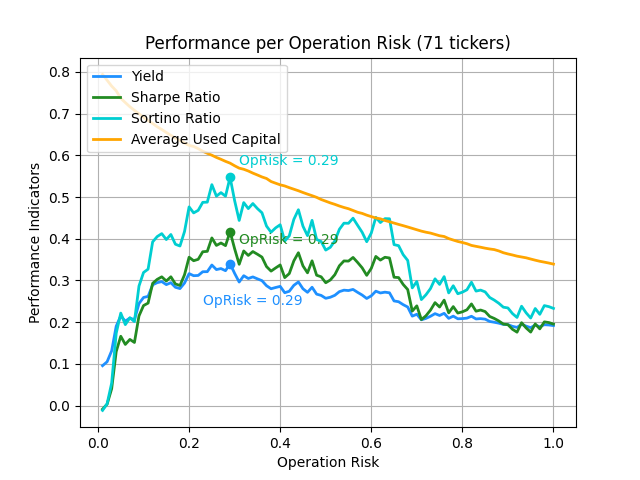
\includegraphics[scale=0.80]{performance_per_op_risks.png}
    \centering
    \caption{Indicadores de performance em função do risco de entrada (71 tickers, 01/01/2019 a 31/12/2021)}
    \label{fig:553}
\end{figure}



\FloatBarrier
\subsection{Período Máximo de Dias por Operação}
\label{sub:max_op_days}

\paragraph{} Em teoria, poderia-se permitir que operações não tivessem um período máximo de dias para serem encerradas. Contudo, isso facilmente se prova uma decisão ruim de alocação de capital em ativos que passam por uma fase de consolidação, ou seja, sem qualquer tendência. Além do ativo em questão não encerrar a operação e finalizar seu lucro ou seu prejuízo na carteira, o capital alocado nele não pode ser utilizado por outros ativos que eventualmente venham a lucrar, ou seja, gera-se um efeito de inércia ao aumento da performance geral. Portanto, foi imposto um limite do período de tempo de todas as operação em um valor máximo.

% \paragraph{} A escolha de um número adequado para o limite de dias possui alguns caminhos, resumidos entre os extremos de: um valor fixo geral; ou um valor dinâmico para cada ação. Nota-se que criar um algoritmo que escolha o valor dinâmico a partir da análise dos dados dos últimos meses para cada ação não é trivial. Assim, optou-se por um valor fixo geral, onde a base do estudo se deu na análise ações de perfis opostos.

% \paragraph{} Embora ações de companhias apresentem comportamentos distintos, optou-se por um valor fixo geral, onde o ponto de partida do estudo de um valor adequado se deu através da análise ações de perfis opostos.

\paragraph{} Nesta linha, um algoritmo auxiliar foi criado para varrer um período de dias passados e criar operações com diversos valores de risco, observando quais riscos levariam a operações de sucesso e quais levariam a operações de falha. Também analisou-se a distribuição de operações de sucesso de acordo com os valores de risco e o intervalo de dias corridos.

\paragraph{} De início, foi fixado um intervalo máximo de 90 dias para cada operação hipotética que o algoritmo gerou. O valor é propositalmente excessivo, pois sua função é apenas não forçar \textit{timeout} na maioria das operações. As Figuras \ref{fig:120} e \ref{fig:121} mostram dois histogramas dos dias das operações de sucesso que consideram o menor risco possível, isto é, o menor valor de risco que se pode utilizar a cada dia da série temporal de forma a tornar a operação um sucesso, caso ele exista. Se não existir, é considerado operação de falha, portanto está fora dos histogramas. A legenda indica faixas onde, no caso da linha tracejada em verde na Figura \ref{fig:120}, 50\% das contagens se encontram dentro dos 12 primeiros dias, e assim por diante.

\begin{figure}[!htb]
    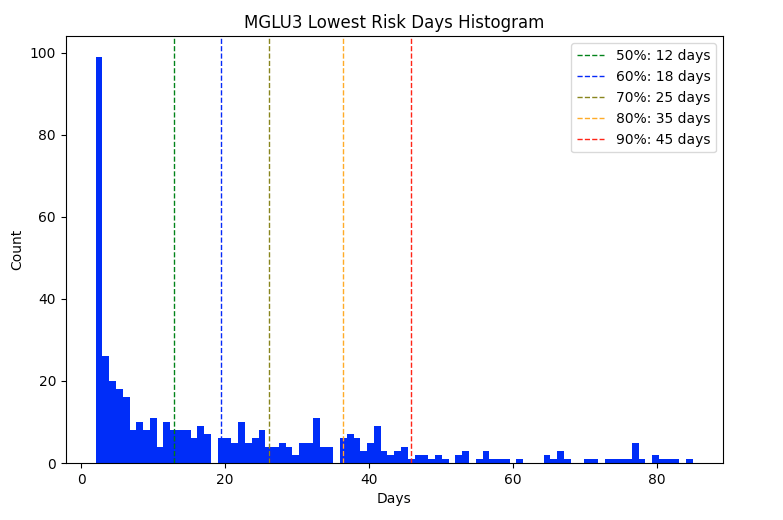
\includegraphics[scale=0.40]{MGLU3_stop_hist_min_risk.png}
    \centering
    \caption{MGLU3 - Histograma de dias com risco mínimo em operações de sucesso (01/01/2016 a 31/12/2018)}
    \label{fig:120}
\end{figure}

\begin{figure}[!htb]
    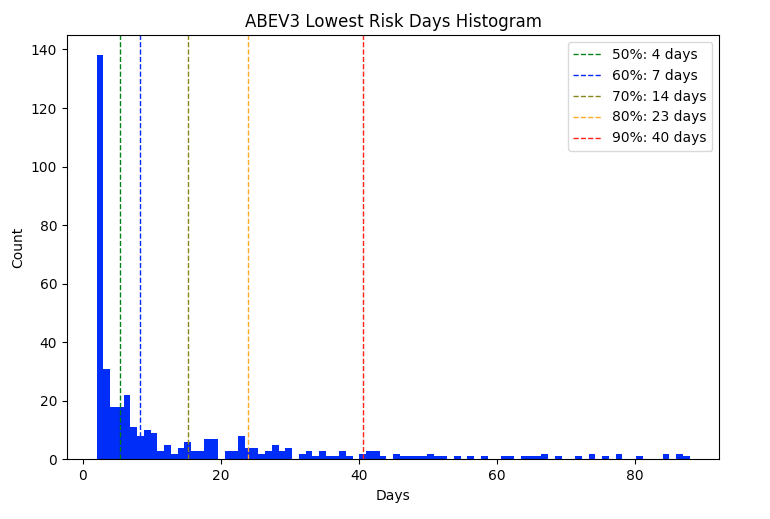
\includegraphics[scale=0.40]{ABEV3_stop_hist_min_risk.png}
    \centering
    \caption{ABEV3 - Histograma de dias com risco mínimo em operações de sucesso (01/01/2016 a 31/12/2018)}
    \label{fig:121}
\end{figure}

\paragraph{} Também foram analisados os histogramas de risco ótimo por operação, ou seja, o valor de risco que traz o melhor rendimento por operação considerando os dias corridos (Figuras \ref{fig:122} e \ref{fig:123}).

\begin{figure}[!htb]
    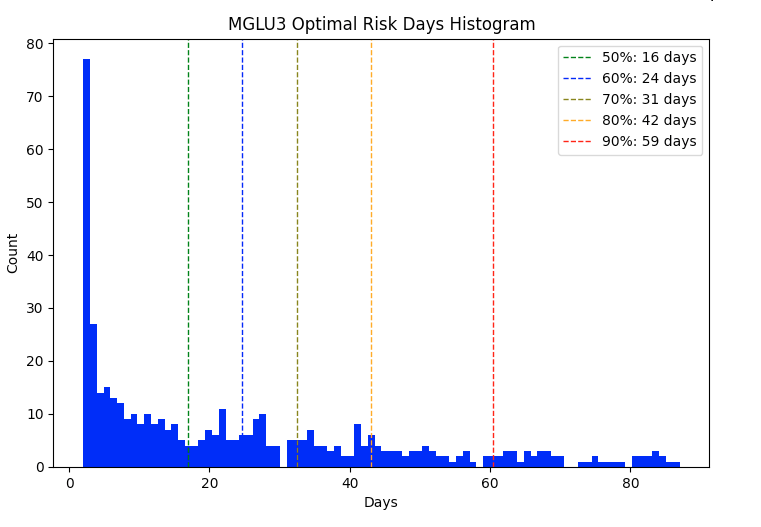
\includegraphics[scale=0.40]{MGLU3_stop_hist_opt_risk.png}
    \centering
    \caption{MGLU3 - Histograma de dias com risco ótimo em operações de sucesso (01/01/2016 a 31/12/2018)}
    \label{fig:122}
\end{figure}

\begin{figure}[!htb]
    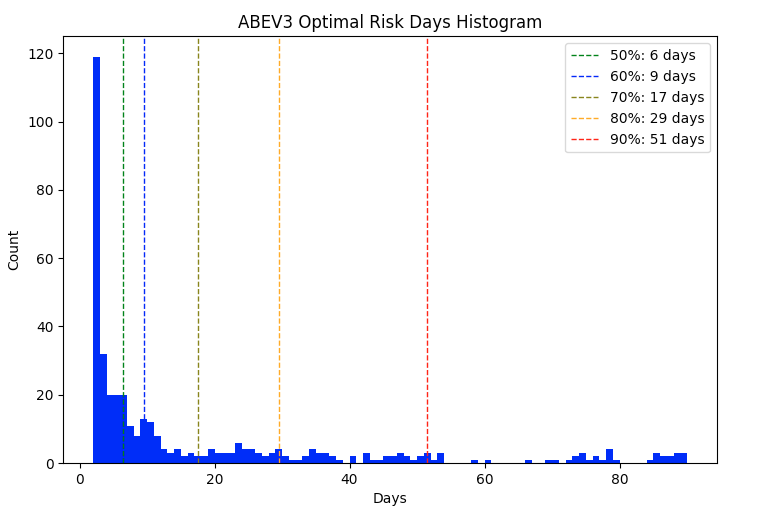
\includegraphics[scale=0.40]{ABEV3_stop_hist_opt_risk.png}
    \centering
    \caption{ABEV3 - Histograma de dias com risco ótimo em operações de sucesso (01/01/2016 a 31/12/2018)}
    \label{fig:123}
\end{figure}

A Figura \ref{fig:540} mostra a distribuição de todas as operações de sucesso possíveis no intervalo selecionado. Obseva-se que valores baixos de risco não costumam estar associados a longos períodos de operação e que a maior densidade de operações de sucesso se encontra em baixo risco e em baixa duração de operação.

\begin{figure}[!htb]
    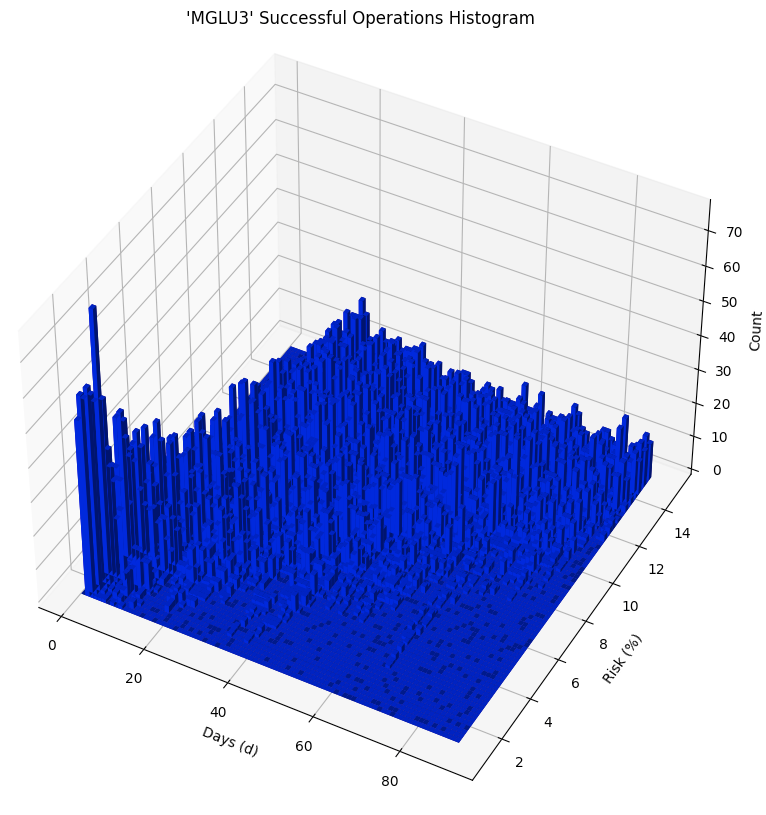
\includegraphics[scale=0.40]{riskmap_mglu3.png}
    \centering
    \caption{MGLU3 - Histograma de todas as operações de sucesso (01/01/2016 a 31/12/2018)}
    \label{fig:540}
\end{figure}

A Tabela \ref{tab:4} resume o período de dias que engloba 90\% das contagens dos histogramas conforme indicado nas Figuras \ref{fig:120}, \ref{fig:121}, \ref{fig:122} e \ref{fig:123}.

\begin{table}[h!]
    \begin{center}
        \begin{tabular}{ c|cc }
            & Menor Risco & Risco Ótimo \\
            \hline
            MGLU3 & 45 dias & 59 dias \\
            ABEV3 & 40 dias & 51 dias \\
        \end{tabular}
        \caption{Período de dias que engloba 90\% das contagens dos histogramas}
        \label{tab:4}
    \end{center}
\end{table}

% \paragraph{} Com base nos valores encontrados, escolheu-se como ponto de partida o período máximo de \textbf{45 dias} para qualquer operação. Esse valor será melhor depurado na Seção \ref{sub:escolha_param} e se necessário, substituído por outro mais adequado.
\paragraph{} Na tentativa de encontrar o valor bem ajustado para o Período Máximo de Dias, uma simulação com o parâmetro ajustado para o intervalo de 1 a 90 dias foi executada para os 71 \textit{tickers} da Tabela \ref{tab:5} para o período de 01/01/2019 a 31/12/2021. Utilizou-se um RCC de 0,22\% para evitar saturação de capital e nenhuma otimização. A Figura \ref{fig:740} mostra os resultados obtidos. Os máximos dos indicadores de performance coincidem em 45 dias de Período Máximo de Dias uma vez que os modelos utilizados na simulação foram criados a partir de \textit{datasets} que utilizavam este valor como limite de suas operações artificiais (Seção \ref{sub:dataset_gen}). \color{red} HERALDO: Basicamente confirmei o esperado. O problema de testar outros valores é que seria necessário gerar os datasets para valores diferentes de 45 dias e recriar os modelos. A criação completa de uma leva de modelos (71 tickers-01/2019 a 12/2021) demora pouco mais de 2 dias de execução em um PC quad-core e ocupa 490MB em ZIP. \color{black}

\begin{figure}[!htb]
    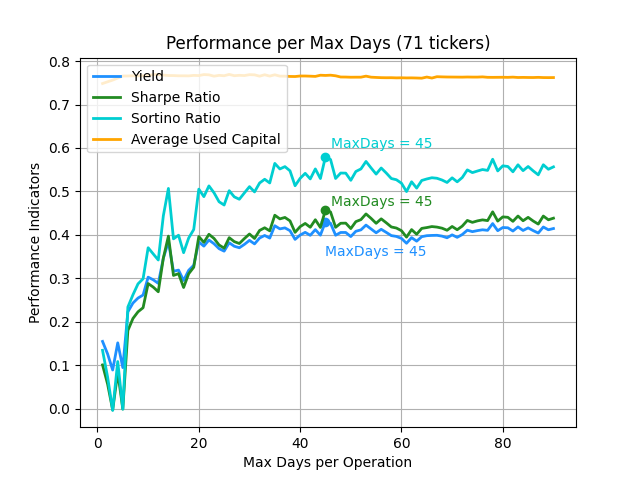
\includegraphics[scale=0.80]{performance_per_max_days.png}
    \centering
    \caption{Análise do Período Máximo de Dias por Operação (71 \textit{tickers} - 01/01/2019 a 31/12/2021)}
    \label{fig:740}
\end{figure}




\FloatBarrier
\subsection{Descanso por Tendência de Baixa}
\label{sub:downtrend_halt}

\paragraph{} O Descanso por Tendência de Baixa é um intervalo que impede qualquer nova operação durante a ativação do \textit{Flag} de Tendência de Baixa (ver Seção \ref{sub:features}). O objetivo é esperar o mercado entrar em uma nova tendência de alta ou pelo menos se estabilizar para que uma nova operação se justifique, mesmo que esta decisão implique em uma pequena inércia. Operações em vigor não são canceladas. \color{red} HERALDO: Optei por não colocar uma imagem mostrando a eficácia desse flag porque em princípio a Seção de Features (\ref{sub:features}) já faz isso. \colorend



\FloatBarrier
\subsection{Descanso por Identificação de Crises}
\label{sub:crisis_halt}

\paragraph{} O Descanso por Identificação de Crises é um intervalo que impede qualquer nova operação durante a ativação do \textit{Flag} de Identificação de Crises (ver Seção \ref{sub:features}). O objetivo é esperar o mercado se estabilizar de uma crise em potencial para que uma nova operação se justifique, mesmo que esta decisão implique em uma pequena inércia. Operações em vigor não são canceladas. \color{red} HERALDO: Optei por não colocar uma imagem mostrando a eficácia desse flag porque em princípio a Seção de Features (\ref{sub:features}) já faz isso. \colorend



\FloatBarrier
\subsection{Lista de Parâmetros de Configuração}
\label{sub:params_list}

\paragraph{} A Tabela \ref{tab:3} mostra uma lista de todos os parâmetros configuráveis em uma simulação. Nota-se que as variáveis de escopo geral são aplicáveis a toda e qualquer estratégia presente no Arquivo de Configuração enquanto as variáveis de escopo local dizem respeito apenas a um grupo de estratégias em parciluar (ver Seção \ref{sub:conf_file}).

\begin{center}
    {\small
    \begin{longtable}[m]{| m{11em} | m{21em} |}

        \hline
        \multicolumn{2}{|c|}{Lista de Parâmetros} \\
        \hline
        Nome do Parâmetro & Descrição \\
        \hline
        \endfirsthead

        \hline
        \multicolumn{2}{|c|}{Continuação da Tabela \ref{tab:3}} \\
        \hline
        Nome do Parâmetro & Descrição \\
        \hline
        \endhead

        \hline
        \endfoot

        \hline
        \multicolumn{2}{|c|}{Fim da Tabela \ref{tab:3}} \\
        \hline
        \caption{Lista de parâmetros detalhados\label{tab:3}}
        \endlastfoot

        \hline
        % show\_results & Geral & Exibe \textit{dashboard} da última simulação completada ao final. Tipo: \textit{Boolean}. \textit{Default}: \textit{True}. Listável: Não. \\
        % \hline
        % min\_risk\_features & Geral & Risco mínimo para o cálculo de \textit{features}. Tipo: \textit{Float}. \textit{Default}: 0,01. Listável: Não. \\
        % \hline
        % max\_risk\_features & Geral & Risco máximo para o cálculo de \textit{features}. Tipo: \textit{Float}. \textit{Default}: 0,10. Listável: Não. \\
        % \hline
        \textbf{name} & \textbf{(OBRIGATÓRIO)} Nome da estratégia a ser executada. Único valor válido: ``ML". Tipo: \textit{String}. Listável: Não. \\
        \hline
        \textbf{alias} & \textbf{(OBRIGATÓRIO)} Rótulo de Identificação. Tipo: \textit{String}. \textit{Default}: \textit{String} vazia. Listável: Não. \\
        \hline
        \textbf{stock\_targets} & \textbf{(OBRIGATÓRIO)} \textit{Array} de ações a incluir na carteira. Formato indicado pela Figura \ref{fig:101}. \\
        \hline
        comment & Comentário. Tipo: \textit{String}. \textit{Default}: \textit{String} vazia. Listável: Não. \\
        \hline
        capital & Capital total da carteira em reais (R\$). Tipo: \textit{Float}. \textit{Default}: 100000. Listável: Sim. \\
        \hline
        risk\_capital\_coefficient & Coeficiente de risco-capital (RCC) geral (Seção \ref{sub:risk_man}). Tipo: \textit{Float}. \textit{Default}: 0,001. Listável: Sim. \\
        \hline
        % tickers\_bag & Critério de escolha do grupo de ativos a escolher dentro de ``stock\_targets". Valores aceitos: ``listed\_first" (ordem de listagem); ``random" (ordem aleatória). \textit{Default}: ``listed\_first". Listável: Sim. \\
        % \hline
        % tickers\_number & Número de ativos a escolher dentro de ``stock\_targets", de acordo com ``tickers\_bag". Tipo: \textit{Int}. \textit{Default}: 0 (todos). Listável: Sim. \\
        % \hline
        tickers\_number & Número de ativos a escolher dentro de ``stock\_targets" em ordem de listagem. Tipo: \textit{Int}. \textit{Default}: 0 (todos). Listável: Sim. \\
        \hline
        min\_order\_volume & Volume mínimo por operação. Tipo: \textit{Int}. \textit{Default}: 1. Listável: Sim. \\
        \hline
        % gain\_loss\_ratio & Razão entre ganho e perda. Para uma unidade de risco (delta pencentual entre preço de compra e \textit{stop loss}) são utilizadas N unidades de risco acima no preço preço de compra para definir o preço alvo. Tipo: \textit{Float}. \textit{Default}: 3. Listável: Sim. \\
        % \hline
        max\_days\_per\_operation & Número máximo de dias por operação (Seção \ref{sub:max_op_days}). Inclui o dia de compra. Caso excedido, ocorre venda compulsória pelo preço de fechamento no último dia da contagem. Tipo: \textit{Int}. \textit{Default}: 45. Listável: Não. \\
        \hline
        min\_risk & Risco mínimo por operação. Tipo: \textit{Float}. \textit{Default}: 0,003. Listável: Sim. \\
        \hline
        max\_risk & Risco máximo por operação. Tipo: \textit{Float}. \textit{Default}: 0,15. Listável: Sim. \\
        \hline
        operation\_risk & Valor percentual de escolha do risco de entrada em operação (Seção \ref{sub:operation_risk}). Tipo: \textit{Float}. \textit{Default}: 0,5. Listável: Sim. \\
        \hline
        enable\_frequency\hspace{2em} \_normalization & Uso de normalização por frequência de operações (Seção \ref{sub:freq_norm}). Tipo: \textit{Boolean}. \textit{Default}: \textit{False}. Listável: Sim. \\
        \hline
        enable\_profit\hspace{4em} \_compensation & Uso de compensação por lucratividade acumulada (Seção \ref{profit_comp}). Tipo: \textit{Boolean}. \textit{Default}: \textit{False}. Listável: Sim. \\
        \hline
        enable\_downtrend\_halt & Uso de descanso por identificação de tendência de baixa (Seção \ref{sub:downtrend_halt}). Tipo: \textit{Boolean}. \textit{Default}: \textit{False}. Listável: Sim. \\
        \hline
        enable\_crisis\_halt & Uso de descanso por identificação de crises (Seção \ref{sub:crisis_halt}). Tipo: \textit{Boolean}. \textit{Default}: \textit{False}. Listável: Sim. \\
        \hline
        enable\_dynamic\_rcc & Uso de Coeficiente de Risco-Capital dinâmico (Seção \ref{sub:dynamic_rcc}). Tipo: \textit{Boolean}. \textit{Default}: \textit{False}. Listável: Sim. \\
        \hline
        dynamic\_rcc\_reference & Valor de referência de uso de capital médio no controle do RCC dinâmico (Seção \ref{sub:dynamic_rcc}). Tipo: \textit{Float}. \textit{Default}: 1,0. Listável: Sim. \\
        \hline
        dynamic\_rcc\_k & Valor do ganho proporcional K no controle do RCC dinâmico (Seção \ref{sub:dynamic_rcc}). Tipo: \textit{Float}. \textit{Default}: 10. Listável: Sim. \\
        \hline

        % purchase\_margin & Margem percentual aplicada ao valor de compra. Ex: Se o alvo de compra estiver configurado para R\$100, uma margem de 1\% permitirá a compra antecipada em R\$99. Tipo: \textit{Float}. \textit{Default}: 0. Listável: Sim. \\
        % \hline
        % stop\_margin & Margem percentual aplicada ao valor do \textit{stop loss}. Ex: Se o \textit{stop} estiver configurado para R\$100, uma margem de 1\% permitirá a compra antecipada em R\$101. Tipo: \textit{Float}. \textit{Default}: 0. Listável: Sim. \\
        % \hline
        % partial\_sale & Uso de saídas parciais. Tipo: \textit{Boolean}. \textit{Default}: \textit{False}. Listável: Sim. \\
        % \hline
        % stop\_type & Tipo de \textit{stop loss} utilizado. Valores aceitos: ``normal"; ``staircase" (para cada patamar de unidade de risco que o preço atinge acima do valor de compra, o \textit{stop} sobe igualmente, até uma unidade de risco abaixo do preço alvo). Ver ``gain\_loss\_ratio". \textit{Default}: ``normal". Listável: Sim. \\
        % \hline
        % min\_days\_after\_successful \_operation & Mínimo de dias sem novas aquisições após operação de sucesso, para cada ação. Ex: para 1 dia mínimo, se a última venda de sucesso ocorreu durante o dia X, a próxima compra só ocorrerá a partir do dia X+2, inclusive. Tipo: \textit{Int}. \textit{Default}: 0. Listável: Sim. \\
        % \hline
        % min\_days\_after\_failure \_operation & Mínimo de dias sem novas aquisições após operação de falha, para cada ação. Ex: para 1 dia mínimo, se a última venda de falha ocorreu durante o dia X, a próxima compra só ocorrerá a partir do dia X+2, inclusive. Tipo: \textit{Int}. \textit{Default}: 0. Listável: Sim. \\
        % \hline

    \end{longtable}}
\end{center}



\FloatBarrier
\subsection{Ensaios Paralelos}

\color{red} HERALDO: Vou fazer apenas fazer comentários para te mostrar o caminho que seguirei caso você julgue que valha a pena trabalhar essa seção. \colorend

\paragraph{} Alguns parâmetros não se mostraram eficazes em melhorar a performance das simulações, muito embora tenham se apresentado como alternativas plausíveis na resolução de problemas ao longo deste trabalho. São eles os parâmetros:

\begin{itemize}
    \item Venda Parcial (partial\_sale)
    \color{red} HERALDO: A motivação da criação desse parâmetro vem de uma prática do André como uma forma de auxiliar o fator psicológico do trader para os casos frustantes em que o mercado quase chega no preço de venda, mas depois cai e bate no stop. Ele não usa isso constantemente, mas deixa como uma opção. Venda parcial em uma operação é vender 50\% do volume de compra adquirido quando o preço bater uma unidade de risco (1un Risco = Pcompra - StopLoss) acima do preço de compra. Dessa forma, ao invés da operação ter um ganho de 3X para cada X de possível perda, ela teria um ganho de 2X para os mesmos X, mais os casos de saída sem prejuízo. A grande questão é que essa conta não compensa, seja quando eu estava tentando replicar a estratégia do André, seja com os modelos de ML agora, nunca trouxe um rendimento maior. \colorend

    \item Saídas Parcias (stop\_type = ``staircase")
    \color{red} HERALDO: É uma extensão que criei derivada da Venda Parcial para tentar granularizar um pouco mais o critério anterior e verificar se o problema da ineficácia estava na escolha do limiar de venda. Igualmente não traz melhora alguma. A ideia é: cada vez que o preço de marcado toca o limiar de uma unidade de risco (1un Risco = Pcompra - StopLoss) acima do preço de compra, o stop loss sobre igualmente 1 un de risco. Exemplo: se o preço de compra é Pcom e o Stop Loss é Pcom - X, quando o preço de mercado atingir Pcom + X, o Stop Loss sobe para Pcom. Quando subir de novo para Pcom + 2X, o Stop sobe para Pcom + X. O alvo continua sendo Pcom + 3X como sempre. \colorend

    \item Dias Mínimos de Espera após Operação de Falha (min\_days\_after\_failure\_operation)

    \item Dias Mínimos de Espera após Operação de Sucesso (min\_days\_after\_successful\_operation)
    \color{red} HERALDO: A motivação de ambos os parâmetros aqui era diminuir o ruído de entrada e saída em operações sequenciais que o modelo de ML arrisca, mas toda hora a operação é stopada. São regiões do gráfico que apresentam 2, 3, 4 operações de falha curtas e seguidas, eventualmente com uma de sucesso e já volta pra falha. Na minha interpretação, os motivos da existência dessas regiões tem a ver com a qualidade do modelo, porém mais especificamente com: (1) a semelhança forte do momento presente com um passado de treinamento onde houve muito sucesso, muito embora possa ser apenas coincidência; e (2) a escolha de um valor de risco de entrada muito baixo para a volatilidade atual do mercado, porém sufiente para o modelo arriscar a operação (pode se somar aqui o efeito indicado em (1)). Moral da história: algumas vezes funcionou (com modelos anteriores que já discartei), porém mesmo QUANDO funciona, é difícil ter clareza do número ótimo de dias para ambos os parâmetros. Digo isso pois acontece do valor de dias escolhido estar em uma região da curva instável onde a melhora do rendimento geral foi coincidência. A prova disso se dá quando você escolhe valores imediatamente próximos e verifica novos resultados discrepantes (simulando sempre com os 71 tickers em uma carteira de 100000 reais). Enfim, eles estão sempre aqui como opções, mas são são consistentes. \colorend
\end{itemize}



\FloatBarrier
\subsection{\textit{Dashboard}}

\paragraph{} Um \textit{Dashboard} interativo é gerado por aplicação secundária a fim de auxiliar a análise dos resultados obtidos em cada simulação. O \textit{framework} \textit{Dash} \cite{dash} foi utilizado para criar uma interface web resumindo todas as informações pertinentes a uma simulação executada. As Figuras \ref{fig:171}, \ref{fig:172}, \ref{fig:173}, \ref{fig:174} e \ref{fig:175} mostram em partes as seções de uma simulação genérica.

\begin{figure}[!htb]
    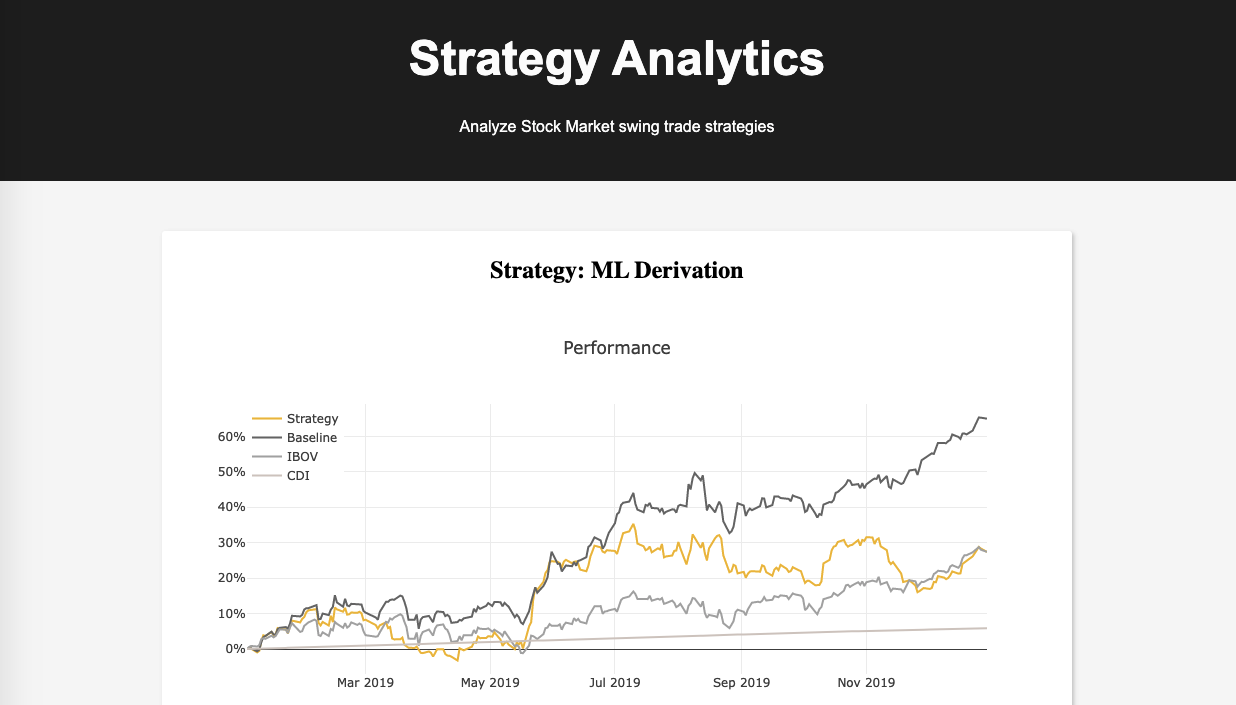
\includegraphics[scale=0.33]{dash_1.png}
    \centering
    \caption{\textit{Dashboard} - Performance}
    \label{fig:171}
\end{figure}

\begin{figure}[!htb]
    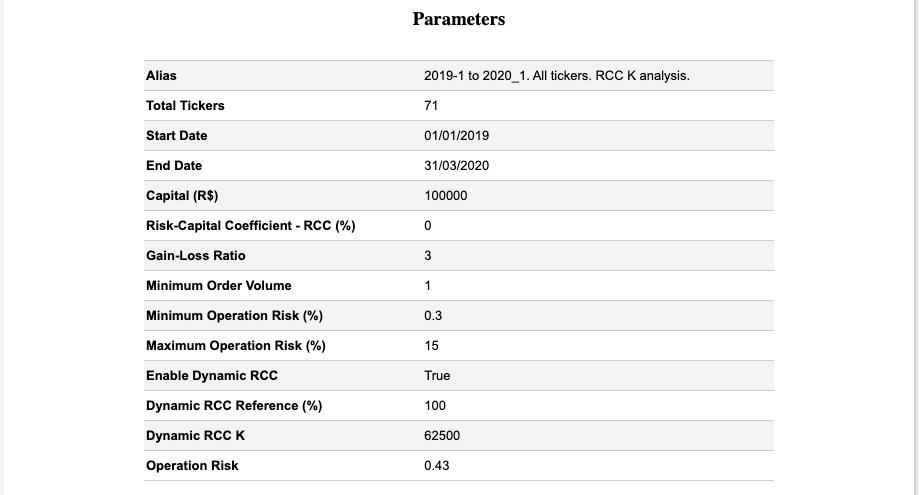
\includegraphics[scale=0.33]{dash_2.png}
    \centering
    \caption{\textit{Dashboard} - Parâmetros de entrada}
    \label{fig:172}
\end{figure}

\begin{figure}[!htb]
    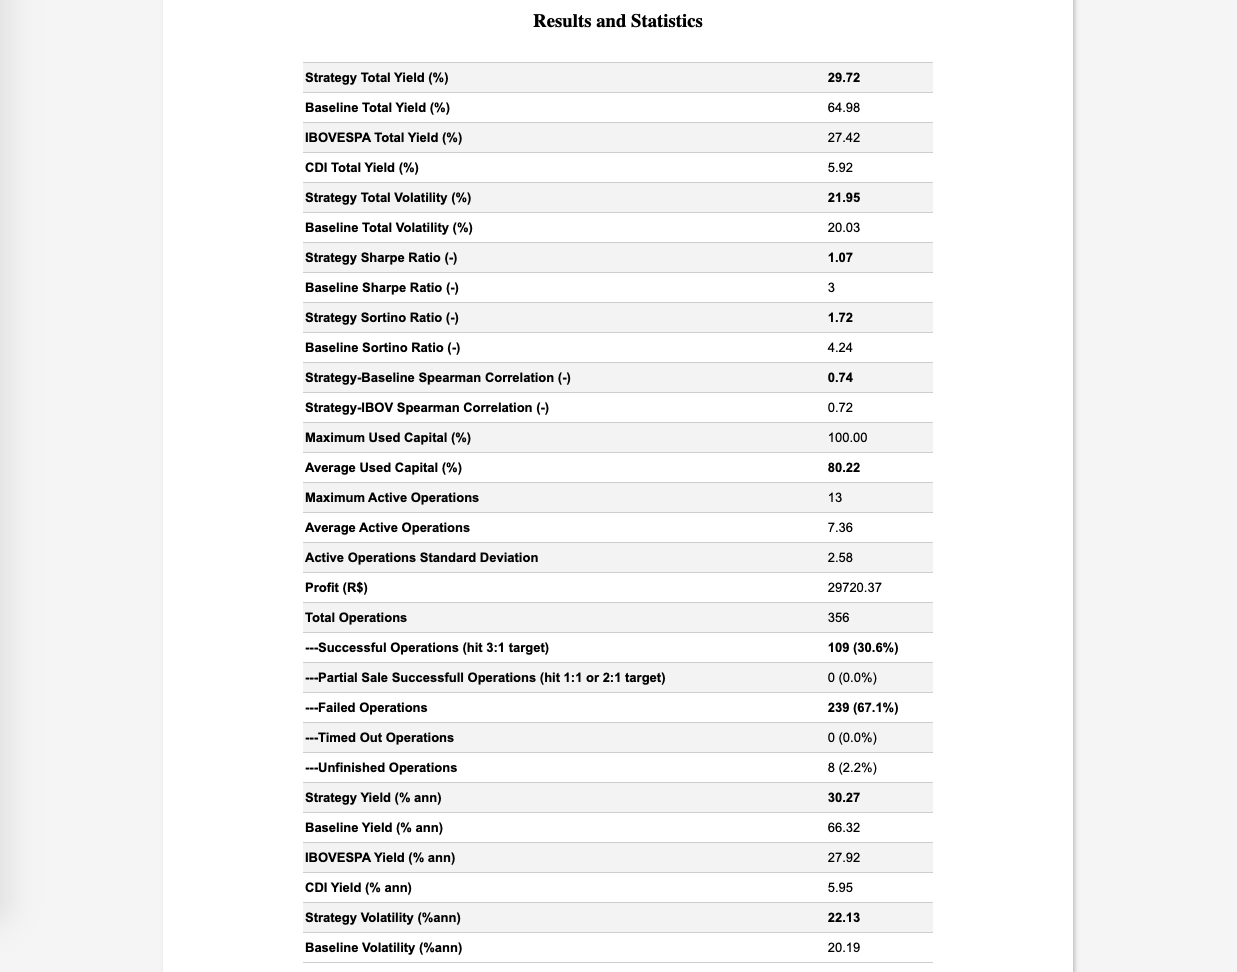
\includegraphics[scale=0.33]{dash_3.png}
    \centering
    \caption{\textit{Dashboard} - Resultados e estatísticas}
    \label{fig:173}
\end{figure}

\begin{figure}[!htb]
    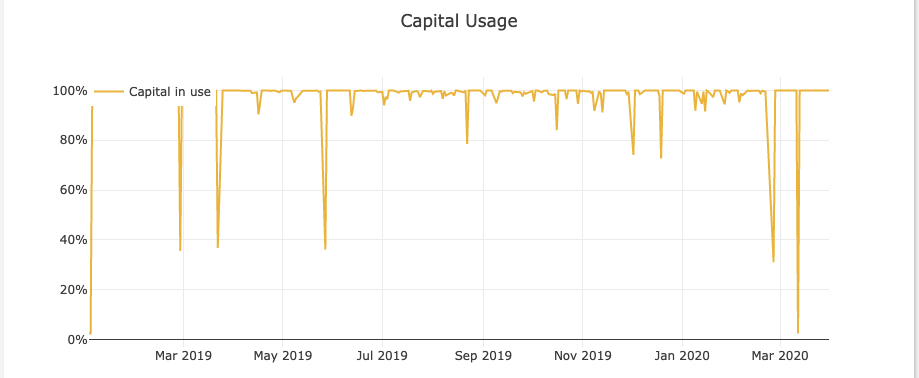
\includegraphics[scale=0.33]{dash_4.png}
    \centering
    \caption{\textit{Dashboard} - Gráfico de uso de capital}
    \label{fig:174}
\end{figure}

\begin{figure}[!htb]
    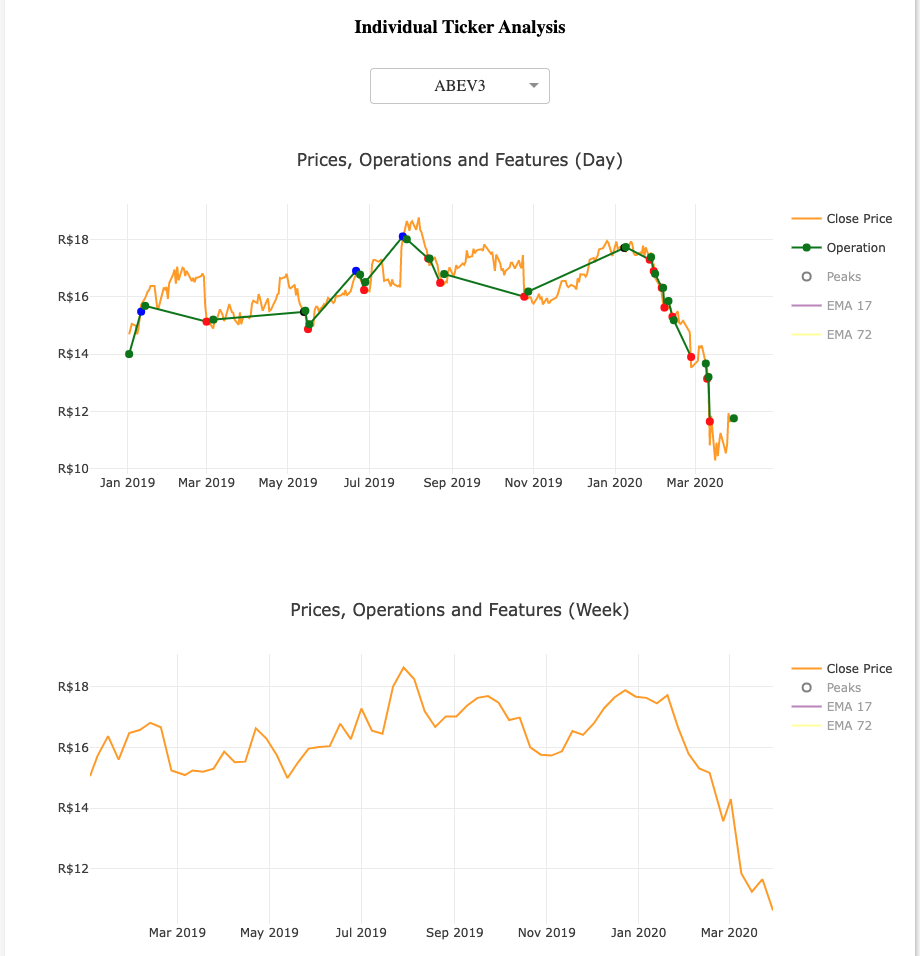
\includegraphics[scale=0.33]{dash_5.png}
    \centering
    \caption{\textit{Dashboard} - Gráficos de análise individual de ações }
    \label{fig:175}
\end{figure}



\FloatBarrier
\section{Otimizações de Gerenciamento de Carteira}



\FloatBarrier
\subsection{Resumo}

\paragraph{} As otimizações apresentadas nesta Seção independem de um modelo de ML específico, sendo portanto algoritmos gerais que, motivados ou não por problemas oriundos dos modelos, buscam uma abordagem geral para aumento da performance da carteira.



% \subsection{Normalização por Frequência de Operações}
% \label{sub:freq_norm}

% \paragraph{} Cada ativo de uma carteira possui um critério próprio de análise das condições de mercado que o auxilia na decisão de entrada nas operações. Muitas vezes, ativos diferentes acumulam um número bastante variado de operações concluídas ao longo da simulação. O ponto esse número não posui ligação direta com a performance individual dos mesmos. Em outras palavras, facilmente ocorre a situação de um \textit{ticker} monopolizar grande parte do capital total da carteira ao longo do tempo, simplesmente por ter uma frequência de operações maior que os outros, sem qualquer fator meritocrático que embase uma justificativa.

% \paragraph{} A fim de se endereçar essa questão, foi criado o critério de Normalização por Frequência de Operações, onde cada ativo receberá de capital para uma determinada operação um valor inversamente proporcional a frequência de operações acumulada até o momento.

% \paragraph{} As Equações \ref{eq:80} e \ref{eq:81} mostram a obtenção do novo Capital Normalizado \begin{math} Capital_{norm} \end{math} a partir: do capital que em princípio seria alocado (Equação \ref{eq:61}); da frequência média de operações totais acumuladas pela carteira \begin{math} \overline{f_{total}} \end{math}; e da frequência média de operações do ativo envolvido \begin{math} f_{stock} \end{math}, igualmente acumulada.

% \begin{equation} \label{eq:80}
%     Capital_{norm} = Capital \times \dfrac{ \overline{f_{total}} }{ f_{stock}}
% \end{equation}

% \begin{equation} \label{eq:81}
%     \overline{f_{total}} = \dfrac{ N_{total\_operations} }{ N_{total\_stocks} }
% \end{equation}

% \paragraph{} Para a Normalização começar a ser aplicada a um ativo, é necessário que haja pelo menos uma operação concluída do mesmo, assim como um mínimo equivalente ao total de ativos na carteira em operações concluídas. A Equação \ref{eq:82} mostra as condições citadas.

% \begin{equation} \label{eq:82}
%     f_{stock} > 0, \quad N_{total\_operations} \ge N_{total\_stocks}
% \end{equation}

% \paragraph{} A Figura \ref{fig:130} mostra a eficácia do critério criado para a simulação dos 71 \textit{tickers} listados na Tabela \ref{tab:5}, durante o período de 01/01/2019 a 31/12/2021, onde a linha em verde denominada de \textit{benchmark} indica a ausência da Normalização e a linha em amarelo denominada por \textit{yield} indica a presença da Normalização.

% \begin{figure}[!htb] % ID: 408, 407
%     
\includegraphics[scale=0.70]{no_image.jpeg}
%     \centering
%     \caption{Simulação sem uso da Normalização por Frequência de Operações}
%     \label{fig:130}
% \end{figure}

% \begin{table}[h!]
%     \begin{center}
%         \begin{tabular}{ c|c|ccc }
%             Norm. por Freq. & Uso Médio de Cap. & Rend. Final & Sharpe & Sortino \\
%             \hline
%             Não & 68,70\% & 36,71\% & 0,4 & 0,49 \\
%             Sim & 69,23\% & 34,58\% & 0,37 & 0,44 \\
%         \end{tabular}
%         \caption{Comparação de Resultados}
%         \label{tab:6}
%     \end{center}
% \end{table}

% \paragraph{} A Figura \ref{fig:131} é análoga à Figura \ref{fig:130}, com a diferença que ambas as execuções estão com o Densanso por Tendência de Baixa e Descando por Identificação de crises ativados.

% \begin{figure}[!htb] % ID: 409, 410
%     
\includegraphics[scale=0.70]{no_image.jpeg}
%     \centering
%     \caption{Simulação com uso da Normalização por Frequência de Operações}
%     \label{fig:131}
% \end{figure}

% % \paragraph{} A Tabela \ref{tab:6} traz um comparativo dos resultados das simulações. Observa-se que o critério de Normalização criado se auto-compensa, ou seja, realoca capital dentro da própria estratégia sem grandes alterações no Uso Médio de Capital da carteira. A vantagem de um critério auto-compensado é que ele não traz uma potencial ilusão de melhora de performance, já que a comparação de resultados entre estratégias precisa ter em vista Usos Médios de Capital razoavelmente próximos entre si para que a escolha dos RCCs individuais não influencie a análise.

% % \begin{table}[h!]
% %     \begin{center}
% %         \begin{tabular}{ c|cc }
% %             & hue & hue \\
% %             \hline
% %             hue & hue & hue \\
% %             hue & hue & hue \\
% %         \end{tabular}
% %         \caption{Comparação de Resultados}
% %         \label{tab:6}
% %     \end{center}
% % \end{table}

% % \paragraph{} (Mencionar mais comentários sobre os outros parâmetros quando tiver as imagens e a tabela).



\FloatBarrier
\subsection{Compensação por Lucratividade}
\label{profit_comp}

% \paragraph{} A Compensacão por Lucratividade é um ajuste auto-compensado\footnote{Realoca capital dentro da própria estratégia sem alterar o Uso Médio de Capital da carteira} que aumenta o capital em operações de \textit{tickers} que possuem um lucro acumulado acima da média da carteira. Da mesma forma, também diminui o capital daqueles que estão com o lucro acumulado abaixo da média da carteira.
\paragraph{} A Compensacão por Lucratividade é um ajuste cujo objetivo está no aumento de capital em operações de \textit{tickers} que possuem um lucro acumulado acima da média da carteira, assim como na diminuição de capital daqueles que estão com o lucro acumulado abaixo da média da carteira.

\paragraph{} A Equação \ref{eq:90} mostra a primeira etapa do cálculo da Compensação, onde \begin{math} \sigma_{eq} \end{math} é o valor em unidades de desvio padrão do quanto o lucro acumulado \begin{math} p_t \end{math} do ativo está em relação à média \begin{math} \overline{P_w} \end{math} e desvio padrão \begin{math} \sigma_w \end{math} da carteira.

\begin{equation} \label{eq:90}
    \sigma_{eq} = \dfrac{p_t - \overline{P_w}}{\sigma_w}
\end{equation}

\paragraph{} Em seguida, a Equações \ref{eq:91} e \ref{eq:92} dão sequência ao cálculo criando os coeficientes das retas que serão utilizadas diretamente na Compensação através da Figura \ref{fig:140}. Nota-se que \begin{math} C_{max} \end{math} é a variação máxima positiva que a Compensação pode alcançar. \begin{math} \sigma_s \end{math} e \begin{math} \sigma_e \end{math} são limiares de \begin{math} \sigma_{eq} \end{math} que definem lugares geométricos diferentes.

\begin{equation} \label{eq:91}
    m_1 = \dfrac{ C_{max} }{ \sigma_e - \sigma_s }, \quad n_1 = 1 - \sigma_s m_1
\end{equation}

\begin{equation} \label{eq:92}
    m_2 = \dfrac{ C_{max} }{ \sigma_e - \sigma_s }, \quad n_2 = 1 + \sigma_s m_2
\end{equation}

\paragraph{} Finalmente, a Equação \ref{eq:93} mostra o cálculo final, que pode ser facilmente visualizado pela Figura \ref{fig:140}.

\begin{equation} \label{eq:93}
    C = \begin{cases} m_1 \sigma_{eq} + n_1, & \mbox{se } \sigma_{eq} \ge \sigma_s \quad \textrm{e} \quad \sigma_{eq} \le \sigma_e \\ m_2 \sigma_{eq} + n_2, & \mbox{se } \sigma_{eq} \le - \sigma_s \quad \textrm{e} \quad \sigma_{eq} \ge - \sigma_e \\ 1 + C_{max}, & \mbox{se } \sigma_{eq} > \sigma_e \\ 1 - C_{max}, & \mbox{se } \sigma_{eq} < - \sigma_e \\ 0, & \mbox{se } |\sigma{eq}| < \sigma_s \end{cases}
\end{equation}

\pgfmathsetmacro{\cmax}{0.6}
\pgfmathsetmacro{\sigs}{0.2}
\pgfmathsetmacro{\sige}{2.0}

\begin{figure}[!htb]
    \centering
    \begin{center}
        \begin{tikzpicture}
            \begin{axis}
            [
                ylabel={Compensa\c{c}\~ao [-]},
                xlabel={$Lucro [\sigma_{eq}]$},
                xmin=-3, xmax=3,
                ymin=0, ymax=2,
                xtick={-3, -2, -1, 0, 1, 2, 3},
                ytick={0, 0.2, 0.4, 0.6, 0.8, 1, 1.2, 1.4, 1.6, 1.8, 2.0},
                ymajorgrids=true,
                xmajorgrids=true,
                grid style=dashed,
            ]
            \addplot[line width=0.50mm, domain=-\sigs:\sigs,blue]{1};
            \addplot[line width=0.50mm, domain=\sigs:\sige,blue]{x * \cmax / (\sige - \sigs) + (1 - \cmax * \sigs / (\sige - \sigs))};
            \addplot[line width=0.50mm, domain=-\sige:-\sigs,blue]{x * \cmax / (\sige - \sigs) + (1 + \cmax * \sigs / (\sige - \sigs))};
            \addplot[line width=0.50mm, domain=\sige:10,blue]{1 + \cmax};
            \addplot[line width=0.50mm, domain=-10:-\sige,blue]{1 - \cmax};
            \end{axis}

        \end{tikzpicture}
    \end{center}
    \caption{Gráfico da Função de Compensação por Lucratividade}
    \label{fig:140}
\end{figure}

\paragraph{} Utilizou-se \begin{math} C_{max} = 0.60\end{math}, \begin{math} \sigma_s = 0.2 \end{math} e \begin{math} \sigma_e = 2.0 \end{math}.

\paragraph{} A Figura \ref{fig:141} mostra o ganho de performance obtido para a simulação dos 71 \textit{tickers} listados na Tabela \ref{tab:5} durante o período de 01/01/2019 a 31/12/2021. A linha em amarelo indica a simulação com uso da Compensação enquanto a linha verde indica a simulação sem o uso. Nenhuma outra otimização foi utilizada. A Tabela \ref{tab:9} traz um comparativo dos resultados das simulações. Nota-se que o RCC foi ajustado para que o Uso Médio de Capital de ambas simulações ficassem próximos.

% ID: 415 (sem), 414 (com)
\begin{figure}[!htb]
    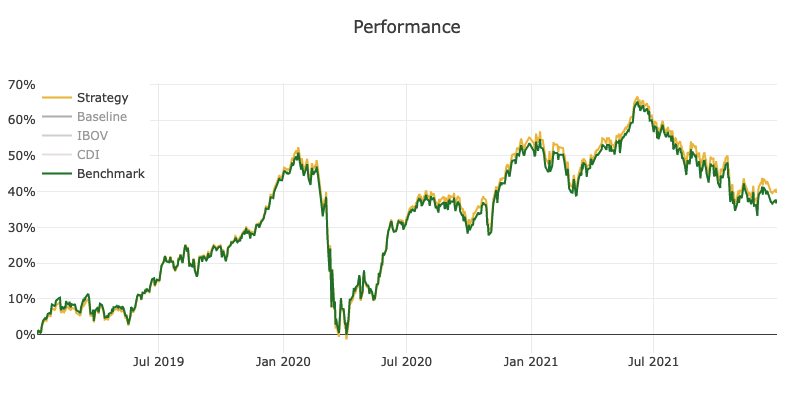
\includegraphics[scale=0.50]{profit_comp.png}
    \centering
    \caption{Performance por uso de Compensação por Lucratividade}
    \label{fig:141}
\end{figure}

\begin{table}[h!]
    \begin{center}
        \begin{tabular}{ c|cc|ccc }
            Comp. Luc. & RCC & Uso Méd. Cap. & Rend. Final & Sharpe & Sortino \\
            \hline
            Não & 0,35\% & 78,30\% & 42,06\% & 0,43 & 0,52 \\
            Sim & 0,22\% & 78,74\% & 44,58\% & 0,46 & 0,55 \\
        \end{tabular}
        \caption{Compensação por Lucratividade - Comparação de Resultados}
        \label{tab:9}
    \end{center}
\end{table}



\FloatBarrier
\subsection{Controle Proporcional para Uso de Capital}
\label{sub:dynamic_rcc}

% \paragraph{} A criação de um RCC como ferramenta de gerenciamento de risco (ver Seção \ref{sub:risk_man}) não resolve o problema de subaproveitamento do Uso de Capital da carteira ao longo do período de simulação. Entende-se por subaproveitamento a parcela de capital ocioso que, por não estar empregado em nenhum ativo, resulta em uma perda de performance geral.

\paragraph{} A criação de um RCC fixo pode ser interessante do ponto de vista de Gerenciamento de Risco (Seção \ref{sub:risk_man}), mas na prática deixa um pouco a desejar por requerer uma noção prévia de um valor adequado. Esse valor só pode ser obtido através de simulações anteriores ao período desejado, onde o comportamento do mercado pode ser suficientemente diferente a ponto de requerer um novo RCC, dificultando um bom ajuste. Em outras palavras, um RCC fixo pode levar a problemas de subaproveitamento do Uso de Capital da carteira.

\paragraph{} A atenuação desse problema se dá pela criação de um RCC Dinâmico, configurado através de um Controle Proporcional. A vantagem dessa abordagem está na diminuição da sensibilidade do RCC em relação à performance geral, permitindo um ajuste menos preciso sem grande impacto de performance. O Controle atua no rebalanceamento de capital em função do uso médio de capital vigente, ou seja, períodos com menos oportunidades de operações terão mais alavancagem de capital e vice-versa.

% \paragraph{} \color{red} HERALDO: Pensei em colocar um diagrama desse controle proporcional aqui, porém o bloco que representaria a planta (i.e., estratégia) é extremamente não-linear. \colorend

\paragraph{} As Equações \ref{eq:100} e \ref{eq:101} mostram o cálculo do RCC dinâmico (\begin{math} RCC_{din} \end{math}) a partir do RCC fixo (\begin{math} RCC_{fix} \end{math}, definido pela Equação \ref{eq:60}), do valor de referência para o uso médio de capital (\begin{math} C_{ref} \end{math}), da constante de ganho proporcional (\begin{math} K \end{math}) e do uso médio de capital dos últimos 10 dias de simulação (\begin{math} \overline{C_{10d}} \end{math}).

\begin{equation} \label{eq:100}
    e = C_{ref} - \overline{C_{10d}}, \quad \mbox{para } 0 \le C_{ref}, \overline{C_{10d}} \le 1
\end{equation}

\begin{equation} \label{eq:101}
    RCC_{din} = RCC_{fix} (1 + K e)
\end{equation}

% \paragraph{} Foi utilizado \begin{math} C_{ref} = 1.0 \end{math}, \begin{math} K = 10 \end{math} e \begin{math} RCC_{fix} = 0.003 \end{math}

\paragraph{} A Figura \ref{fig:150} mostra o ganho de performance obtido pela implementação do RCC Dinâmico com os valores \begin{math} C_{ref} = 1.0 \end{math}, \begin{math} K = 7,5 \end{math} e \begin{math} RCC_{fix} = 0.0022 \end{math}. A linha em amarelo indica a simulação com uso do RCC Dinâmico enquanto a linha verde indica a simulação sem o uso. Nenhuma outra otimização foi utilizada. A Tabela \ref{tab:10} traz um comparativo dos resultados das simulações. Nota-se que o RCC foi ajustado para que o Uso Médio de Capital de ambas simulações ficassem próximos.

% ID: 420 (sem), 419 (com)
\begin{figure}[!htb]
    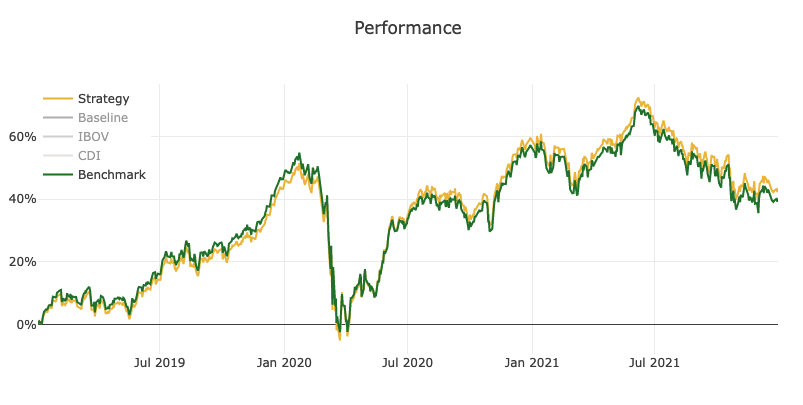
\includegraphics[scale=0.50]{dyn_rcc_no_flags.png}
    \centering
    \caption{Performance por uso de RCC dinâmico sem \textit{flags} de descanso}
    \label{fig:150}
\end{figure}

\begin{table}[h!]
    \begin{center}
        \begin{tabular}{ c|cc|ccc }
            RCC Din. & RCC fixo & Uso Méd. Cap. & Rend. Final & Sharpe & Sortino \\
            \hline
            Não & 0,50\% & 84,20\% & 44,93\% & 0,44 & 0,53 \\
            Sim & 0,22\% & 84,11\% & 47,37\% & 0,47 & 0,57 \\
        \end{tabular}
        \caption{RCC Dinâmico - Comparação de Resultados sem \textit{flags} de descanso}
        \label{tab:10}
    \end{center}
\end{table}

\paragraph{} Analogamente à Figura \ref{fig:150}, a Figura \ref{fig:151} também mostra o ganho de performance, porém na condição de ativação dos Descansos por Tendência de Baixa e por Identificação de Crises para ambas as simulações. A Tabela \ref{tab:11} compara os resultados das simulações.

% ID: 425 (sem), 422 (com)
\begin{figure}[!htb]
    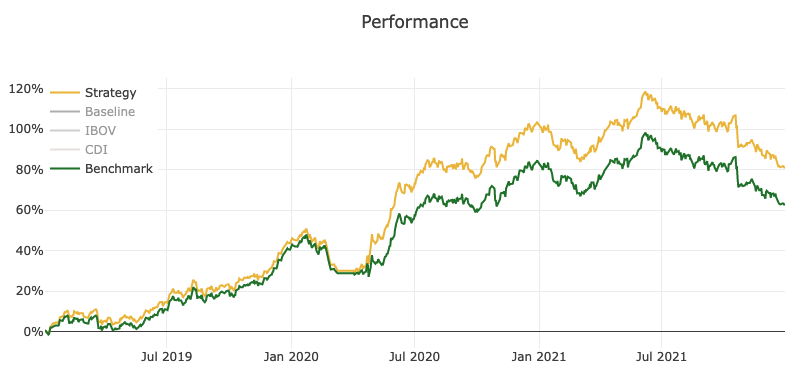
\includegraphics[scale=0.50]{dyn_rcc_with_flags.png}
    \centering
    \caption{Performance por uso de RCC dinâmico com \textit{flags} de descanso}
    \label{fig:151}
\end{figure}

\begin{table}[h!]
    \begin{center}
        \begin{tabular}{ c|cc|ccc }
            RCC Din. & RCC fixo & Uso Méd. Cap. & Rend. Final & Sharpe & Sortino \\
            \hline
            Não & 0,63\% & 73,89\% & 66,61\% & 0,94 & 1,27 \\
            Sim & 0,22\% & 73,98\% & 83,38\% & 1,20 & 1,69 \\
        \end{tabular}
        \caption{RCC Dinâmico - Comparação de Resultados com \textit{flags} de descanso}
        \label{tab:11}
    \end{center}
\end{table}

\paragraph{} A Figura \ref{fig:560} mostra o gráfico da relação entre os indicadores de performance em função do RCC para todos os 71 \textit{tickers} da Tabela \ref{tab:5}. Os pontos marcados representam os máximos dos respectivos gráficos. Observa-se que o melhor K se encontra no intervalo [13, 16]. Portanto, o valor escolhido é a média dos limites do intervalo: 14,5. \color{red} HERALDO: O que acha da escolha da média? \color{black}

\begin{figure}[!htb]
    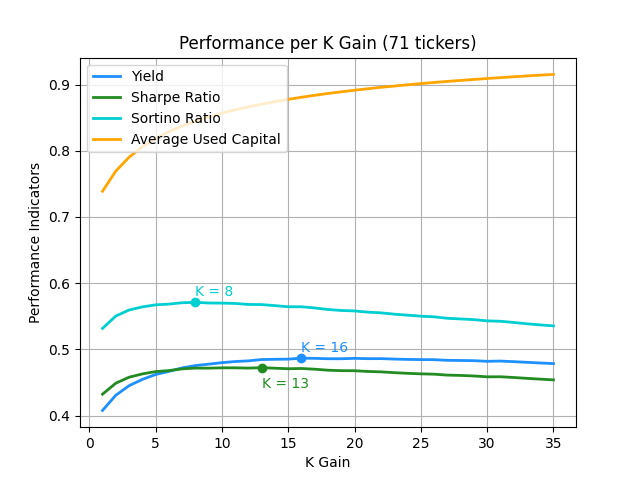
\includegraphics[scale=0.80]{performance_per_rcc_k.png}
    \centering
    \caption{Indicadores de performance em função do ganho K (71 tickers: 01/01/2019 a 31/12/2021)}
    \label{fig:560}
\end{figure}



\FloatBarrier
\section{Modelos de Aprendizado Supervisionado}



\FloatBarrier
\subsection{Resumo}

\paragraph{} A partir de \textit{datasets} previamente populados, modelos do tipo \textit{Random Forest} são gerados para cada ação a cada intervalo de 3 meses de simulação. Um critério particular de performance foi criado para auxiliar na escolha do melhor modelo, que é filtrado por uma varredura de diversos parâmetros.



\FloatBarrier
\subsection{\textit{Datasets} e \textit{Feature Selection}}
\label{sub:dataset_gen}

\paragraph{} Os \textit{datasets} são arquivos CSV criados para cada \textit{ticker} através de uma varredura da série histórica. Analisa-se dia após dia as \textit{features} acumuladas e o resultado de uma operação hipotética iniciada no dia corrente. A Tabela \ref{tab:7} mostra a lista de \textit{features} relevantes do arquivo, onde as linhas marcadas em negrito indicam as colunas utilizadas na entrada de dados dos modelos. A coluna Resultado da Operação indica a saída observada para o treinamento supervisionado.

\begin{table}[h!]
    \begin{center}
        \begin{tabular}{ l|c|c }
            Nome & Coluna & Tipo \\
            \hline
            \textit{Ticker} & ticker & \textit{string} \\
            Início da Operação & day & \textit{datetime} \\
            \textbf{Risco da Operação} & risk & \textit{float} \\
            \textbf{Resultado da Operação} & success\_oper\_flag & \textit{boolean} \\
            \textit{Flag} de Fim de Intervalo & end\_of\_interval\_flag & \textit{boolean} \\
            \textbf{Derivada Preço Médio} & mid\_prices\_dot & \textit{float} \\
            \textbf{\textit{Spearman} (5 dias)} & spearman\_corr\_5\_day & \textit{float}: Preço Médio, f(x)=x \\
            \textbf{\textit{Spearman} (10 dias)} & spearman\_corr\_10\_day & \textit{float}: Preço Médio, f(x)=x \\
            \textbf{\textit{Spearman} (15 dias)} & spearman\_corr\_15\_day & \textit{float}: Preço Médio, f(x)=x \\
            \textbf{\textit{Spearman} (20 dias)} & spearman\_corr\_20\_day & \textit{float}: Preço Médio, f(x)=x \\
            \textbf{\textit{Spearman} (25 dias)} & spearman\_corr\_25\_day & \textit{float}: Preço Médio, f(x)=x \\
            \textbf{\textit{Spearman} (30 dias)} & spearman\_corr\_30\_day & \textit{float}: Preço Médio, f(x)=x \\
            \textbf{\textit{Spearman} (35 dias)} & spearman\_corr\_35\_day & \textit{float}: Preço Médio, f(x)=x \\
            \textbf{\textit{Spearman} (40 dias)} & spearman\_corr\_40\_day & \textit{float}: Preço Médio, f(x)=x \\
            \textbf{\textit{Spearman} (50 dias)} & spearman\_corr\_50\_day & \textit{float}: Preço Médio, f(x)=x \\
            \textbf{\textit{Spearman} (60 dias)} & spearman\_corr\_60\_day & \textit{float}: Preço Médio, f(x)=x \\
        \end{tabular}
        \caption{Comparação de Resultados}
        \label{tab:7}
    \end{center}
\end{table}

\paragraph{} O termo preço médio se refere ao definido pela Equação \ref{eq:22}. Da mesma forma, a derivada do preço médio é indicada pela Equação \ref{eq:23}. As colunas de cujos nomes se iniciam com \textit{Spearman} são na verdade a correlação entre o vetor de preços médios dos últimos N dias acumulados e uma função puramente monotônica crescente \begin{math} f(x) = x \end{math}. Isso permite a extração de uma medida para intensidade de subida dos preços que independe da normalização pelo preço da ação. Como o que importa na correlação de Spearman são os postos, o valor númerico do vetor utilizado para representar a função \begin{math} f(x) = x \end{math} não tem relevância, desde que seja monotônico crescente.

\paragraph{} O \textit{flag} de fim de intervalo indica que, pelo fato do \textit{dataset} ter chegado ao final, não é possível dizer se a operação foi de sucesso ou foi de falha, portanto a mesma é desconsiderada do treinamento.

\paragraph{} Por fim, para cada dia de operação, foram cruzadas diversas opções de risco a fim de enriquecer o \textit{dataset} com mais diversidade, permitindo modelos mais robustos. Foram utilizadas 119 opções de risco: de 0,2\% a 12\% em passos de 0,1\%.



\FloatBarrier
\subsection{Índice de Lucratividade}

% \paragraph{} Durante a etapa de criação dos modelos, é necessário uma métrica para ranqueamento das performances que acompanhe o contexto, pois não se trata de um simples problema de classificação de um \textit{dataset} balanceado onde ambas as classes possuem o mesmo peso perante o enredo no qual se inserem. Na verdade, o \textit{dataset} é bastante desbalanceado, chegando a casa dos 90\% de operações de falha em comparação às operações de sucesso em alguns casos. Além disso, o impacto de um acerto por parte do modelo implica em um ganho de 3X para a carteira, onde X é o valor de entrada da operação. Assim como uma falha implica em uma perda de -X para a carteira.
\paragraph{} Durante a etapa de criação dos modelos, é necessário uma métrica para ranqueamento das performances que acompanhe o contexto. O impacto de um acerto por parte do modelo implica em um ganho de 3X para a carteira, onde X é o valor de entrada da operação. Assim como uma falha implica em uma perda de -X para a carteira.

\paragraph{} O Índice de Lucratividade é um coeficiente entre 0 e 1 onde 0 significa o pior resultado possível, isto é, aquele no qual o modelo errou todas as operações no \textit{dataset} de forma a trazer o maior prejuízo possível. Por outro lado, 1 significa o maior lucro que o modelo pode trazer se acertar todas as operações que o \textit{dataset} permite. Nota-se que o valor do Índice que representa o lucro zero não é necessariamente 0.5, e sim algum valor intermediário que precisa ser fornecido durante o cálculo. Também é importante ressaltar que como os \textit{datasets} variam entre si, os valores de lucro zero também mudam, portanto a métrica é útil para criação de modelos que utilizem exatamente a mesma fonte de dados.

\paragraph{} Seja A o número de operações de sucesso no \textit{dataset} (classe 1) e B o número de operações de falha (classe 0), pode-se definir \begin{math} S_a \end{math} como a soma dos riscos de todas as operações da classe 1 e \begin{math} S_b \end{math} a soma dos riscos de todas as operações da classe 0. Assim, a Equação \ref{eq:170} representa uma função linear responsável por mapear o lucro \begin{math} L_m \end{math} de um modelo no Índice de Lucratividde.

\begin{equation} \label{eq:170}
    I_{L} = \dfrac{1}{(S_a - S_b)}L_m - \dfrac{S_b}{(S_a - S_b)}
\end{equation}

\paragraph{} O lucro \begin{math} L_m \end{math} pode ser encontrado através da Equação \ref{eq:171}, onde TP é a contagem de verdadeiros positivos do modelos e FN é a contagem de falsos negativos. Falsos positivos e verdadeiros negativos são desconsiderados do cálculo pois como não geram operações, não trazem ganho ou perda alguma.

\begin{equation} \label{eq:171}
    L_m = 3 \times TP - FN
\end{equation}

\paragraph{} Por fim, o valor do Índice que representa o lucro zero pode ser encontrado a partir da Equação \ref{eq:170}, basta impor a condição \begin{math} L_m=0 \end{math} (Equação \ref{eq:172}).

\begin{equation} \label{eq:172}
    I_{L_0} = - \dfrac{S_b}{(S_a - S_b)}
\end{equation}



\FloatBarrier
\subsection{Balanceamento de Classes}

\paragraph{} Devido ao desbalanceamento dos \textit{datasets} utilizados, que pode chegar até cerca de 90\% de operações de falha contra 10\% de operações de sucesso, faz-se imprescindível alguma técnica de balanceamento mencionada na Seção \ref{sub:class_prob}: \textit{undersampling}, \textit{oversampling} ou CSL. A natureza do problema também deve ser levada em consideração, pois um simples balanceamento via CSL daria a mesma importância à predição dos acertos e das falhas, no entanto o impacto de um acerto por parte do modelo gera um ganho de 3X para a carteira e uma falha gera uma perda de -X para os mesmos X apostados.

\paragraph{} Levando em consideração as questões levantadas, optou-se por um balanceamento em cascada de 2 níveis:

\begin{itemize}
    \item \textit{Undersampling} via \textit{Tomek Links}\footnote{Algoritmo que remove amostras da classe majoritária via identificação de \textit{links}. Um \textit{link} entre a amostra A da classe 1 e a amostra B da classe 2 é encontrado se o vizinho mais próximo de A é B e vice-versa \cite{he2013imbalanced}.}, de cujo impacto na proporção das classes é muito pequeno.
    \item CSL levando em considerações o número de amostras e o impacto das classes para a carteira (Tabela \ref{tab:8}).
\end{itemize}

\begin{table}[h!]
    \begin{center}
        \begin{tabular}{ l|c|c|c }
            Classe & Amostras & Peso p/ Carteira & Balanceamento \\
            \hline
            Op. de Falha (Classe 0) & \begin{math} N_0 \end{math} & 1 & \begin{math} \dfrac{(1/4)N_1}{(N_0+(1/4)N_1)} \end{math} \\
            Op. de Sucesso (Classe 1) & \begin{math} N_1 \end{math} & 4 & \begin{math} \dfrac{N_0}{(N_0+(1/4)N_1)} \end{math} \\
        \end{tabular}
        \caption{Balanceamento via CSL}
        \label{tab:8}
    \end{center}
\end{table}


\FloatBarrier
\subsection{Geração de Modelos}

\paragraph{} Os modelos \textit{Random Forest} foram criados a partir da biblioteca \textit{Scikit-Learn} \cite{scikit}. Para a escolha do modelo a ser utilizado na simulação final, diversos outros modelos temporários foram criados e excluídos a fim de se selecionar apenas o melhor. Todos modelos temporários compartilham os parâmetros fixos indicados pela Tabela \ref{tab:15}, porém diferem quanto aos parâmetros variáveis da Tabela \ref{tab:16} ou quanto às sementes aleatórias utilizadas. A lógica de criação dos modelos pode ser interpretada da seguinte forma:

\begin{itemize}
    \item Para cada um dos 71 \textit{tickers} da carteira (Tabela \ref{tab:5}), o período completo de simulação vai de 01/01/2019 a 31/12/2021 e é dividido em 12 intervalos de 3 meses (WFA).

    \item Cada intervalo de 3 meses de simulação é governado pelo melhor modelo de ML criado previamente.

    \item Por trás de cada modelo final selecionado existem 100 modelos temporários organizados em dois níveis: parâmetros variáveis e sementes aleatórias.

    \item O primeiro nível de diferenciação é dado parâmetros variáveis da Tabela \ref{tab:16}, ou seja, as combinações entre \textit{max\_depth} e \textit{max\_features}, que geram os 10 pares (3, 3), (3, 4), (4, 3), (4, 4), ..., (7, 4).

    \item Para cada par criado, são criados 10 modelos com 10 sementes aleatórias diferentes.

    \item O modelo final escolhido possui os mesmos parâmetros do grupo de 10 modelos de sementes aleatórias diferentes que possuir o maior \begin{math} I_L / \sigma_{I_L} \end{math}. \color{red} HERALDO: E o modelo final é o de semente aleatória = 1. \color{black}
\end{itemize}

\begin{table}[!htb]
    \begin{center}
        \begin{tabular}{ l|c }
            Parâmetro & Valor \\
            \hline
            n\_estimators & 200 \\
            criterion & gini \\
            min\_samples\_split & 24 \\
            min\_samples\_leaf & 12 \\
            min\_weight\_fraction\_leaf & 0.0 \\
            max\_leaf\_nodes & None \\
            min\_impurity\_decrease & 0.0 \\
            bootstrap & True \\
            oob\_score & False \\
            warm\_start & False \\
            % class\_weight & balanced\_subsample \\
            ccp\_alpha & 0.0 \\
            max\_samples & None \\
        \end{tabular}
        \caption{Parâmetros fixos}
        \label{tab:15}
    \end{center}
\end{table}

\begin{table}[!htb]
    \begin{center}
        \begin{tabular}{ l|c }
            Parâmetro & Valor \\
            \hline
            max\_depth & [3, 4, 5, 6, 7] \\
            max\_features & [3, 4] \\
        \end{tabular}
        \caption{Parâmetros variáveis}
        \label{tab:16}
    \end{center}
\end{table}

\paragraph{} A Figura \ref{fig:580} ilustra a lógica de criação dos modelos apresentada através de um diagrama. O período de treinamento e de teste de cada modelo foi separado utilizando WFA e pode ser verificado pela Tabela \ref{tab:17}. Entende-se por validade o período de tempo durante a simulação no qual o algoritmo criado pode atuar. Desta forma, cada ação na carteira possui 12 modelos com validade de 3 meses cada.

\begin{figure}[!htb]
    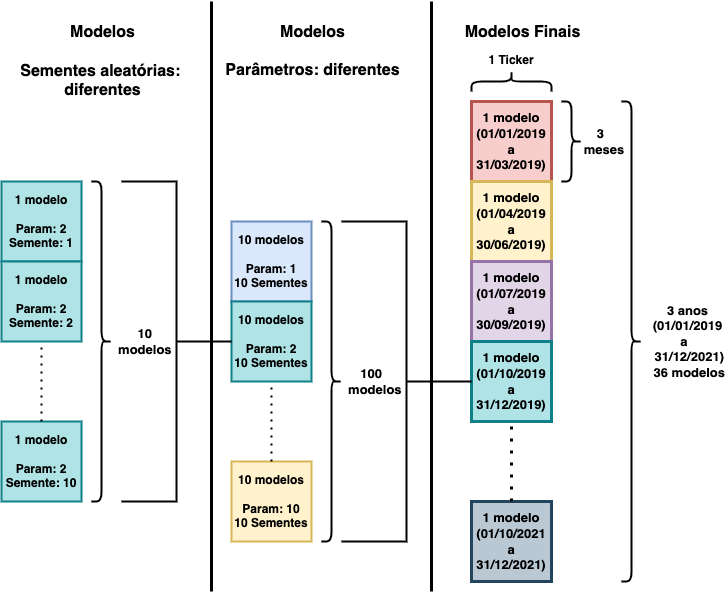
\includegraphics[scale=0.50]{models_chart.png}
    \centering
    \caption{Diagrama de criação de modelos}
    \label{fig:580}
\end{figure}

\begin{table}[!htb]
    \begin{center}
        \begin{tabular}{ cc|cc|cc }
            \multicolumn{2}{c|}{Treinamento} & \multicolumn{2}{c|}{Teste} & \multicolumn{2}{c}{Validade} \\
            \hline
            Início & Fim & Início & Fim & Início & Fim \\
            \hline
            01/01/2013 & 31/03/2018 & 01/04/2018 & 31/12/2018 & 01/01/2019 & 31/03/2019 \\
            01/04/2013 & 30/06/2018 & 01/07/2018 & 31/03/2019 & 01/04/2019 & 30/06/2019 \\
            01/07/2013 & 30/09/2018 & 01/10/2018 & 30/06/2019 & 01/07/2019 & 30/09/2019 \\
            01/10/2013 & 31/12/2018 & 01/01/2019 & 30/09/2019 & 01/10/2019 & 31/12/2019 \\
            01/01/2014 & 31/03/2019 & 01/04/2019 & 31/12/2019 & 01/01/2020 & 31/03/2020 \\
            01/04/2014 & 30/06/2019 & 01/07/2019 & 31/03/2020 & 01/04/2020 & 30/06/2020 \\
            01/07/2014 & 30/09/2019 & 01/10/2019 & 30/06/2020 & 01/07/2020 & 30/09/2020 \\
            01/10/2014 & 31/12/2019 & 01/01/2020 & 30/09/2020 & 01/10/2020 & 31/12/2020 \\
            01/01/2015 & 31/03/2020 & 01/04/2020 & 31/12/2020 & 01/01/2021 & 31/03/2021 \\
            01/04/2015 & 30/06/2020 & 01/07/2020 & 31/03/2020 & 01/04/2021 & 30/06/2021 \\
            01/07/2015 & 30/09/2020 & 01/10/2020 & 30/06/2020 & 01/07/2021 & 30/09/2021 \\
            01/10/2015 & 31/12/2020 & 01/01/2021 & 30/09/2021 & 01/10/2021 & 31/12/2021 \\
        \end{tabular}
        \caption{WFA - Intervalos de treinamento, teste e validade dos modelos}
        \label{tab:17}
    \end{center}
\end{table}



\FloatBarrier
\subsection{Modelo \textit{Baseline}}
\label{sub:baseline}

\paragraph{} No contexto de ML, entende-se como \textit{baseline} a linha base de comparação de um modelo. Em outras palavras, é uma estratégia simples e de fácil implementação que traz uma performace razoável de se obter na realidade. Neste caso, utilizou-se a média de performance das ações da carteira, ou seja, supondo-se que o capital inicial fosse igualmente distribuido em cada ação disponível, o rendimento médio destas ações ao longo do tempo é o \textit{baseline}.

\paragraph{} A Figura \ref{fig:170} mostra o \textit{baseline} calculado para os 71 \textit{tickers} indicados na Tabela \ref{tab:5} no intervalo de 01/01/2019 a 31/12/2021. Adicionou-se o iBovespa (Seção \ref{sub:ibov}) e o CDI\footnote{Certificado de Depósito Interbancário. Indexador cujo valor é numericamente muito próximo à taxa básica de juros da economia, a Taxa Selic.} acumulado para fins de comparação. Nota-se a diferença de performance do \textit{baseline} para o iBovespa, o que é razoável já que o \textit{baseline} tem composição fixa e o iBovespa tem uma composição variável tanto na escolha dos ativos quanto em seus respectivos pesos. Além disso, as 71 ações escolhidas são de empresas em maioria presentes no mercado desde 2013, portanto possuem algum grau de consolidação e resiliência. A Tabela \ref{tab:12} mostra os indicadores de performance para o modelo \textit{baseline}.

\begin{figure}[!htb]
    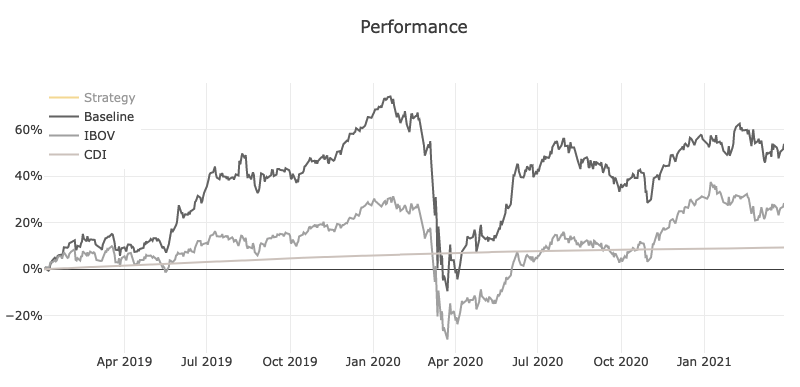
\includegraphics[scale=0.50]{baseline_raw.png}
    \centering
    \caption{\textit{Baseline} para o intervalo de 01/01/2019 a 31/12/2021}
    \label{fig:170}
\end{figure}

\begin{table}[!htb]
    \begin{center}
        \begin{tabular}{ cccc }
            Rend. Final & Volatilidade & Sharpe & Sortino \\
            \hline
            73,94\% & 55,48\% & 0,68 & 0,74 \\
        \end{tabular}
        \caption{\textit{Baseline} - Indicadores de Performance}
        \label{tab:12}
    \end{center}
\end{table}

% \begin{math} R_b \end{math}
% \color{red} HERALDO: \colorend
% \color{red} HERALDO: \color{black}
\chapter{Resultados}
\label{cap4}



\paragraph{} A partir dos modelos criados na Seção \ref{sub:super_models} e dos parâmetros refinados na Seção \ref{sub:est_simulation}, é possível prosseguir com as simulações finais, que compartilham das seguintes configurações:

\begin{itemize}
    \item 71 \textit{tickers} (Tabela \ref{tab:5})
    \item Período de simulação: 01/04/2020 a 31/12/2021
    \item Capital: R\$ 100000,00
    \item Volume mínimo de ações por negociação: 1
    \item Risco de entrada por operação: 0,29
    \item Período máximo de dias por operação: 45
\end{itemize}

\paragraph{} Observa-se que o período de simulação é posterior ao utilizado para refinamento dos parâmetros de simulação (01/01/2019 a 31/12/2020).

\paragraph{} A Tabela \ref{tab:395} mostra 4 perfis de simulação diferentes, cada um motivado por uma questão diferente, são elas: (1) o máximo local na região de baixo RCC da Figura \ref{fig:550}; (2) o máximo local da região de alto RCC, também da Figura \ref{fig:550}; (3) a simulação de maior índice de Shape da Figura \ref{fig:153} pertencente à curva \begin{math} RCC \times K = 1,8 \end{math}; e (4) a simulação de menor perda de operações na Figura \ref{fig:155}, pertencente à curva \begin{math} RCC \times K = 0,1 \end{math}. Também são apresentados os respectivos resultados.

\begin{table}[!htb]
    \begin{center}
        \resizebox{\textwidth}{!}{
        \begin{tabular}{ l|c|c|c|c|c }
            Parâmetro & Estratégia 1 & Estratégia 2 & Estratégia 3 & Estratégia 4 & \textit{Baseline} \\
            \hline
            RCC     & 0,11\%    & 6,10\%    & 0,00288\% & 0,1\% & - \\
            K       & -         & -         & 62500     & 100   & - \\
            \hline
            Rendimento Final                    & \% & \% & \% & \% & 68,07\% \\
            Volatilidade                        & \% & \% & \% & \% & 34,84\% \\
            Índice de Sharpe                    &  &  &  &  & 1,15 \\
            Índice de Sortino                   &  &  &  &  & 1,71 \\
            Cor. Spearman (\textit{Baseline})   &  &  &  &  & - \\
            Cor. Spearman (Ibovespa)            &  &  &  &  & - \\
            Uso Máximo de Capital               & \% & \% & \% & \% & 100\% \\
            Uso Médio de Capital                & \% & \% & \% & \% & 100\% \\
            Máximo de Op. Ativas                &  &  &  &  & 71 \\
            Média de Op. Ativas                 &  &  &  &  & 71 \\
            % Desvio Padrão de Op. Ativas         &  &  &  &  & - \\
            Operações Totais                    &  &  &  &  & 71 \\
            Operações de Sucesso                &  (\%) &  (\%)&  (\%)&  (\%) & - \\
            Operações de Falha                  &  (\%) &  (\%)&  (\%)&  (\%) & - \\
            Operações de \textit{Timeout}       &  (\%) &  (\%)&  (\%)&  (\%) & - \\
            Operações Incompletas               &  (\%) &  (\%)&  (\%)&  (\%) & - \\
        \end{tabular}}
        \caption{Resultados finais}
        \label{tab:395}
    \end{center}
\end{table}


\paragraph{} Cortar daqui para baixo.




% \paragraph{} A partir dos parâmetros descritos e refinados na Seção \ref{sub:est_simulation}, utilizou-se a seguinte configuração para encontrar a simulação com os melhores índices de performance:

% \begin{itemize}
%     \item 71 \textit{tickers} (Tabela \ref{tab:5})
%     \item Período de simulação: 01/01/2019 a 31/12/2021
%     \item Capital: R\$ 100000,00
%     \item Volume mínimo de ações por negociação: 1
%     \item Risco de entrada por operação: 0,29
%     \item Período máximo de dias por operação: 45
%     \item RCC: 0,000025
%     \item Controle Proporcional para Uso de Capital (RCC Dinâmico): Sim
%     \item Valor de Referência: 100\%
%     \item Constante K de Ganho Proporcional: 30000
% \end{itemize}

% \paragraph{} Conforme descrito na Seção \ref{sub:risk_man}, a escolha dos 71 \textit{tickers} foi realizada levando em consideração as seguintes preferências: diversidade de segmentos de mercado; disponibilidade da série temporal de dados a partir de 2013; e presença na composição do iBovespa em qualquer data. O período de simulação escolhido engloba um intervalo recente dos últimos 3 anos, já que a escolha de momentos anteriores a este pode estar associado a padrões de mercado muito diferentes do atual. Como os modelos criados utilizam \textit{walk-forward analysis} e portanto atualizados a cada 3 meses de simulação para cada \textit{ticker}, o comprimento do intervalo de 3 anos não é um problema. O capital e o volume mínimo por negociação foram escolhidos visando evitar potenciais problemas quanto à granularidade dos montantes de negociação.

% \paragraph{} Os demais parâmetros revelam valores refinados através de suas respectivas seções, a mencionar: Seção \ref{sub:operation_risk} para o Risco de entrada por operação; Seção \ref{sub:max_op_days} para o Período máximo de dias por operação; e Seção \ref{sub:dynamic_rcc} para o RCC, o Valor de referência e a Constante K.

\paragraph{} Os resultados encontrados podem ser verificados pela Figura \ref{fig:250} e pela Tabela \ref{tab:13}.

\begin{figure}[!htb]
    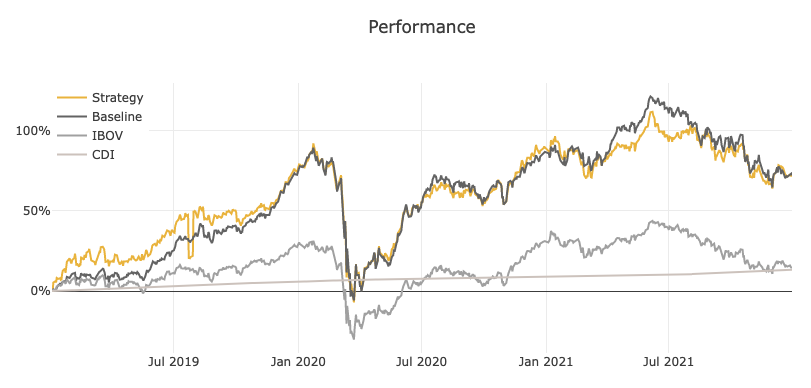
\includegraphics[scale=0.50]{performance_final.png}
    \centering
    \caption{Performance final}
    \label{fig:250}
\end{figure}

\begin{table}[h!] %ID 485
    \begin{center}
        \begin{tabular}{ l|c|c }
            Parâmetro & Estratégia & \textit{Baseline} \\
            \hline
            Rendimento Final & 72,79\% & 73,94\% \\
            Volatilidade & 63,20\% & 55,48\% \\
            Índice de Sharpe & 0,64 & 0,68 \\
            Índice de Sortino & 0,74 & 0,74 \\
            Correlação de Spearman (c/ \textit{Baseline}) & 0,99 & - \\
            Correlação de Spearman (c /Ibovespa) & 0,92 & - \\
            Uso Máximo de Capital & 100\% & 100\% \\
            Uso Médio de Capital & 97,22\% & 100\% \\
            Máximo de Operações Ativas & 71 & - \\
            Média de Operações Ativas & 65,97 & - \\
            Desvio Padrão de Operações Ativas & 6,13 & -\\
            Operações Totais & 3145 & 71 \\
            Operações de Sucesso & 891 (28,3\%) & - \\
            Operações de Falha & 2048 (65,1\%) & - \\
            Operações de \textit{Timeout} & 147 (4,7\%) & - \\
            Operações Incompletas & 59 (1,9\%) & - \\
        \end{tabular}
        \caption{Resultado final}
        \label{tab:13}
    \end{center}
\end{table}

\paragraph{} Deve-se lembar que a estratégia ou o modelo \textit{baseline} é uma representação interna da média de rendimento do mercado para a mesma cesta de ações da estratégia a ser simulada (Seção \ref{sub:baseline}). Com isso em mente, observa-se pela Figura \ref{fig:250} que o rendimento da estratégia final fica em torno do \textit{baseline}, com exceção do primeiro ano de simulação, onde o desempenho é significativamente maior.

\paragraph{} A Tabela \ref{tab:13} também mostra que ambas as estratégias obtiveram resultados bem próximos, em particular a estratégia final teve performance ligeiramente inferior, conforme esperado. Analisando individualmente os resultados, o rendimento da estratégia final está apenas 1,15\% abaixo do \textit{baseline}, o que é relevante, mas não tanto quando se tem em mente que este é apenas o retrato de um dos diversos dias de simulação volátil.

\paragraph{} Apesar dos rendimentos finais equivalentes, não de pode deixar de notar o aumento de volatilidade da estratégia final em 7,72\%, o que prejudica sua qualidade. Contudo, a volatilidade não deve ser analisada isoladamente, mas sim através do índice de Sharpe, que está 0,04 pontos abaixo da referência. Um desvio relevante, porém ainda sutil, mostrando que uma parcela da alta de volatilidade foi compensada por um rendimento médio maior. Já o índice de Sortino está igual em 0,74, mostrando que ambas as estratégias possuem o mesmo grau de confiança quando se analisa a rentabilidade em relação às oscilações de capital abaixo da média.

\paragraph{} Dando sequência à análise, as altas correlações de Spearman mostram uma forte dependência da estratégia em relação ao \textit{baseline} e ao iBovespa, o que pode ser facilmente verificado pela Figura \ref{fig:250}. No entanto, aqui valem algumas ressalvas. Como a correlação de Spearman se baseia apenas nos ranques das funções e não propriamente na magnitude dos valores, é um cenário possível uma estratégia obter uma correlação com o \textit{baseline} muito próxima de 1,0 ao mesmo tempo que um rendimento superior. Isso porque o ganho de capital com cada oscilação positiva seria maior do que a perda em uma oscilação negativa. Por outro lado, também é possível um cenário onde uma estratégia com uma baixa correlação de Spearman com o \textit{baseline} apresente um rendimento superior. Este caso em particular seria um caminho mais interessante, pois mostraria uma versatilidade maior da estratégia criada para diferentes tipos de cenários de mercado.

\paragraph{} O uso máximo de capital em 100\% indica apenas que em algum momento todo capital esteve alocado em ativos. Contudo, o uso médio de capital em 97,22\% traz a informação de que como quase todo capital esteve alocado o tempo todo, há pouco espaço para uma melhora de performance de maneira indiscrimidada daqui para frente. Em outras palavras, as melhoras de rendimento precisarão passar por um aprimoramento dos modelos no que diz respeito a quais operações abrir mão para que outras possam prosperar mais. Nota-se que um uso médio de capital em 100\% não seria vantajoso, uma vez que diminuiria-se a disponibilidade de capital para aporte em novas operações. Por outro lado, um uso médio muito baixo indicaria que a estratégia estaria longe de alcançar o seu máximo potencial de performance. Portanto, uma pequena folga é importante e necessária.

\paragraph{} Assim como o uso médio de capital está alto, a média de operações ativas também está, o que é esperado. O mesmo raciocício vale para o máximo de operações ativas e o uso máximo de capital. \color{red} HERALDO: Não mencionei o Desvio Padrão de Operações Ativas por não achar relevante. Devo removê-lo da tabela? Ou deixo assim mesmo? \color{black}

\paragraph{} Por fim, deve-se ressaltar que o número total de operações de 3145 está saturado, conforme explicado ao final da Seção \ref{sub:dynamic_rcc}. Resumidamente, os parâmetros de simulação, em especial o RCC e o K, estão configurados de forma a estressar a estratégia a ponto dela desobedecer em alguns momentos as ordens de compra vindas dos modelos de ML por falta de capital disponível. Tal abordagem trouxe um aumento de performance, mas deve ser usada com cautela. Independentemente desta questão, a taxa de acerto de 28,3\% contra os 65,1\% de falha mostra que apesar da estratégia acertar pouco, o lucro obtido é proporcionalmente maior que as perdas acumuladas.
\chapter{Validação}
\label{cap5}

\section{Dados de Teste}

\section{Resultados}
\chapter{Conclusão}
\label{cap6}




% ---------------------------------------------------------------
% Bibliografia
% ---------------------------------------------------------------
\normalsize
\cleardoublepage
\addcontentsline{toc}{chapter}{Bibliografia}
\bibliographystyle{coppe}
\bibliography{biblio}


% Apendices

% \appendix

% % Apendice A

% \chapter{O que é um apêndice}
% \label{ApendiceA}
% \chapter{Inconsistência de Proventos na Biblioteca \textit{yfinance}}
\label{ApendiceA}

\paragraph{} Apesar da praticidade de obtenção dos \textit{candlesticks} diários que a biblioteca \textit{yfinance} (Python) traz, seus valores de proventos (dividendos e juros sobre capital próprio) não são totalmente confiáveis. O estudo em questão mostra inconsistências tanto por duplicação quanto por inserção incorreta de proventos. Para isso, uma análise de caso foi realizada para a companhia Magazine Luiza (\textit{ticker} MGLU3), onde foram comparados os dados obtidos do \textit{yfinance} via \textit{script} com o site de relações com investidores da mesma \cite{mglu_ri}. Além disso, utilizou-se a plataforma \textit{TradingView} \cite{tradingview} para confirmação dos valores de preço de fechamento.

% \paragraph{} Referencia \ref{codeA1}

\paragraph{} A Tabela \ref{tab:ap1} mostra o histórico dos preços de fechamento para alguns dias específicos e datas importantes, como distribuição de proventos e desdobramentos \footnote{Em inglês: \textit{split}}, além de outros períodos. A Tabela está ordenada do \textit{candle} mais recente para o mais antigo e as marcações: em vermelho indicam valores incorretos; em azul indicam valores corretos; e em laranja indicam valores que prograparam erros a partir dos valores incorretos. A data de execução do \textit{script} é de 19/09/2020, o que é relevante, uma vez que a plataforma sempre retorna os preços dos \textit{candles} já normalizado por todos os desdobramentos acumulados.


\begin{table}[h!]
    \begin{center}
        \resizebox{\textwidth}{!}{
        \begin{tabular}{ c|ccc|cc|cc }
            Data & Preço Fch            & Preço Fch & Preço Fch             & Provento/Ação     & Provento/Ação & \textit{Split}    & \textit{Split} \\
                 & \textit{yfinance}    & Site RI   & \textit{TradingView}  & \textit{yfinance} & Site RI       & \textit{yfinance} & Site RI \\
                 & (R\$)                & (R\$)     & (R\$)                 & (R\$)             & (R\$/ação)    &                   & \\
            \hline
            16/09/2022 & 4,46 & 4,46 & 4,46 & - & - & - & - \\
            01/07/2022 & 2,20 & 2,20 & 2,20 & - & - & - & - \\
            03/01/2022 & 6,72 & 6,72 & 6,72 & - & - & - & - \\

            07/07/2021 & 22,01 & 22,01 & 22,01 & - & - & - & - \\
            06/07/2021 & 21,07 & 21,07 & 21,07 & \color{blue} 0,015494 \color{black} & 0,0154942583 & - & - \\
            05/07/2021 & 21,3645 & 21,37 & 21,36 & - & - & - & - \\

            04/01/2021 & 25,1817 & 25,18 & 25,18 & - & - & - & - \\
            30/12/2020 & 24,9319 & 24,93 & 24,93 & \color{blue} 0,026301 \color{black} & 0,0263019985 & - & - \\
            29/12/2020 & 25,2354 & 25,24 & 25,24 & - & - & - & - \\

            15/10/2020 & 25,4650 & 25,47 & 25,46 & - & - & - & - \\
            14/10/2020 & 25,6347 & 25,64 & \color{red} 25,54 \color{black} & - & - & \color{blue} 1:4 \color{black} & 1:4 \\
            13/10/2020 & 25,9541 & 25,96 & 25,95 & - & - & - & - \\

            03/08/2020 & 20,6061 & 20,61 & 20,61 & \color{red} 0,094176 \color{black} & - & - & - \\
            31/07/2020 & \color{orange} 20,0479 \color{black} & 20,15 & 20,14 & \color{blue} 0,023541 \color{black} & 0,094165968 & - & - \\
            30/07/2020 & \color{orange} 20,6654 \color{black} & 20,77 & 20,76 & - & - & - & - \\
            29/07/2020 & \color{orange} 19,9012 \color{black} & 20,00 & 19,99 & - & - & - & - \\

            15/04/2020 & \color{orange} 10,8798 \color{black} & 10,93 & 10,93 & - & - & - & - \\
            14/04/2020 & \color{orange} 10,6441 \color{black} & 10,70 & 10,69 & \color{red} 0,179508 \color{black} & - & - & - \\
            13/04/2020 & \color{orange} 10,2203 \color{black} & 10,45 & 10,45 & - & - & - & - \\
            09/04/2020 & \color{orange} 10,1569 \color{black} & 10,39 & 10,38 & - & - & - & - \\

            03/01/2020 & \color{orange} 11,9224 \color{black} & 12,19 & 12,19 & - & - & - & - \\
            02/01/2020 & \color{orange} 12,0297 \color{black} & 12,30 & 12,30 & \color{blue} 0,008947 \color{black} & 0,0357891574 & - & - \\
            30/12/2019 & \color{orange} 11,6235 \color{black} & 11,89 & 11,88 & - & - & - & - \\

            09/10/2019 & \color{orange} 9,6619 \color{black} & 9,88 & 9,88 & - & - & - & - \\
            08/10/2019 & \color{orange} 9,2598 \color{black} & 9,47 & 9,47 & \color{blue} 0,018402 \color{black} & 0,0736066061 & - & - \\
            07/10/2019 & \color{orange} 9,3394 \color{black} & 9,55 & 9,55 & - & - & - & - \\

            06/08/2019 & \color{orange} 8,9016 \color{black} & 9,11 & 9,10 & - & - & \color{blue} 1:8 \color{black} & 1:8 \\

            17/04/2019 & \color{orange} 4,8588 \color{black} & 4,97 & 4,97 & - & - & - & - \\
            16/04/2019 & \color{orange} 4,9463 \color{black} & 5,06 & 5,06 & \color{blue} 0,011571 \color{black} & 0,370259884 & - & - \\
            15/04/2019 & \color{orange} 4,9594 \color{black} & 5,07 & 5,07 & - & - & - & - \\

            03/01/2019 & \color{orange} 5,5812 \color{black} & 5,71 & 5,71 & - & - & - & - \\
            02/01/2019 & \color{orange} 5,6416 \color{black} & 5,77 & 5,77 & \color{blue} 0,018522 \color{black} & 0,59270489 & - & - \\
            28/12/2018 & \color{orange} 5,4744 \color{black} & 5,60 & 5,60 & - & - & - & - \\

        \end{tabular}}
        \caption{Análise de Consistência de Proventos: MGLU3}
        \label{tab:ap1}
    \end{center}
\end{table}

\paragraph{} Analisando a Tabela \ref{tab:ap1} de cima para baixo, nota-se que a primeira irregularidade notável ocorre no dia 14/10/2020, onde a plataforma \textit{TradingView} apresenta um preço de fechamento discrepante em relação ao site de RI da própria companhia e do \textit{yfinance}. Como se trata de um evento singular e não é o foco deste estudo, ele foi desconsiderado.

\paragraph{} Em seguida, nos dias 03/08/2020 e 31/07/2020, o \textit{yfinance} registrou a presença dos proventos de R\$0,094176/ação e R\$0,023541/ação, respectivamente. O problema aqui é que além de ser muito improvável que qualquer empresa na bolsa brasileira distribuia proventos duas vezes em dois dias úteis seguidos, pode-se notar que o valor de R\$0,023541/ação equivalete ao de R\$0,094176/ação quando multiplicado por 4. Em outras palavras, normalizando pelo desdobramento de 1:4 ocorrido em 14/10/2020, conclui-se que um dos proventos é duplicado. Como confirmação, o site de RI da Magazine Luiza dispões de um comunidado sobre a distribuição de proventos de R\$0,094165968/ação em 31/07/2020.

\paragraph{} Continuando a análise, é possível verificar que a partir da duplicata encontrada, os preços de fechamento do \textit{yfinance} vão acumulando o erro. Em 14/04/2020, o \textit{yfinance} contabilizou proventos de R\$0,179508/ação, no entanto, nada foi encontrado no site de RI, o que evidencia um lançamento incorreto. Nota-se também que o valor é relativamente alto quando comparado aos outros proventos de outras datas.

\paragraph{} Os restantes do valores de proventos do \textit{yfinance} em azul equivalem aos comunicados pelo site de RI da companhia, porém deve-se levar em consideração os desdobramentos acumulados.

\paragraph{} Por fim, pode-se concluir que o uso da plataforma \textit{yfinance} no que diz respeito à disponibilização de proventos no contexto deste projeto não pode ser deferida, uma vez que a presença e a magnitude dos valores incorretos não é desprezível.


% \begin{minted}{python}

% import yfinance as yf
% from pathlib import Path

% ticker = 'MGLU3.SA'
% msft = yf.Ticker(ticker)
% hist = msft.history(start='2015-01-01', end='2022-09-19',
%     interval='1d', prepost=False, back_adjust=True, rounding=True)
% destination = Path(__file__).parent / (ticker.upper()+'.csv')
% hist.to_csv(destination)

% \end{minted}


% % Apendice B

% \chapter{Encadernação do Projeto de Graduação}
% \label{ApendiceB}
% \begin{figure}
\begin{center}
\parbox[htb]{13.0cm}
  {
  \begin{center}
  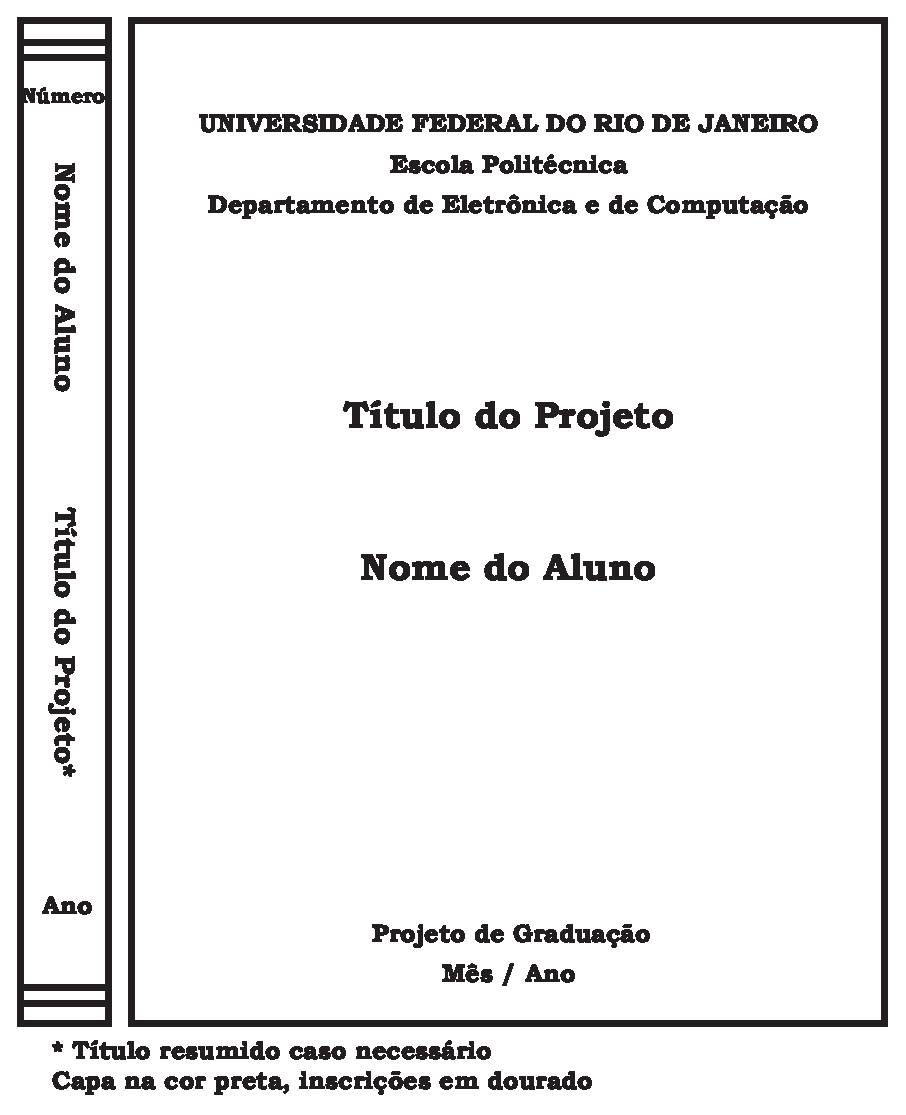
\includegraphics[scale=1.0]{Capa_do_Projeto_Final.eps}
  \caption[\small{Encaderna��o do projeto de gradua��o.}]{\label{FigPFC} \small{Encaderna��o do projeto de gradua��o.}}
  \end{center}
  }
\end{center}
\end{figure}

% % Apendice C

% \chapter{O que é um anexo}
% \label{ApendiceC}
% \paragraph{}Documenta��o n�o elaborada pelo autor, ou elaborada pelo autor mas constituindo parte de outro projeto.

\backmatter

\end{document}